\documentclass{article}

\usepackage{amsmath}
\usepackage{amsfonts}
\usepackage{amssymb}
\usepackage{graphicx}
\usepackage{pgfplots}
\usepackage{subcaption}
\usepackage[colorinlistoftodos]{todonotes}
\usepackage[colorlinks=true, allcolors=blue]{hyperref}
\usepackage[margin=1in]{geometry}

\usepackage{tikz}
\usetikzlibrary{positioning}
\usetikzlibrary{shapes,arrows}
\usepackage{adjustbox}
\tikzstyle{decision} = [diamond, draw, fill=blue!20,
        text width=4.5em, text badly centered, node distance=3cm, inner sep=0pt]
        \tikzstyle{block} = [rectangle, draw, fill=blue!20,
                text width=6em, text centered, rounded corners, minimum height=4em]
                \tikzstyle{line} = [draw, -latex']
                \tikzstyle{cloud} = [draw, ellipse,fill=red!20, node distance=3cm,
                        minimum height=2em]

\graphicspath{ {figures/} }

\pgfmathdeclarefunction{gauss}{2}{%
  \pgfmathparse{exp(-((x-#1)^2)/(2*#2^2))}%
}

\pgfmathdeclarefunction{multimodal}{2}{%
  \pgfmathparse{0.7*exp(-((x-#1)^2)/(2))+0.3*exp(-((x-#2)^2)/(2))}%
}

\pgfplotsset{every tick label/.append style={font=\small}}

\usepackage{algorithm}
\usepackage[noend]{algpseudocode}

% Commands
\newcommand{\alphabet}{\mathcal{A}}
\newcommand{\partis}{\texttt{partis}}
\newcommand{\igor}{\texttt{IGoR}}
\newcommand{\igblast}{\texttt{IgBlast}}
\newcommand{\median}{\operatorname{median}}

% http://bytesizebio.net/2013/03/11/adding-supplementary-tables-and-figures-in-latex/
\newcommand{\beginsupplement}{%
        \setcounter{table}{0}
        \renewcommand{\thetable}{S\arabic{table}}%
        \setcounter{figure}{0}
        \renewcommand{\thefigure}{S\arabic{figure}}%
     }

\title{\texttt{sumrep}: a summary statistic framework for immune receptor repertoire comparison and model validation}
\author{Branden Olson, Software WG folks, Frederick A Matsen IV}

\begin{document}

%BJO - I realize that I alternate between IGoR and "\texttt{igor}" throughout the document, as well as IgBlast vs \texttt{igblast}. Do you have a preference, Erick? I believe I'm consistent with writing \texttt{partis} throughout.
%EM I prefer \texttt{IGoR} etc. I made you some commands above. Note that you'll need `\igor\ ` with a trailing backslash to get a space after the command.

\maketitle

\begin{abstract}
The adaptive immune system generates an incredible diversity of antigen receptors for B and T cells to keep dangerous pathogens at bay.
The DNA sequences coding for these receptors arise by a complex recombination process followed by a series of binding-based filters, as well as affinity maturation for B cells, giving considerable structure to the circulating pool of receptor sequences.
Although these data sets hold considerable promise for medical and public health application, the complex structure of the resulting immune repertoire sequencing (Rep-Seq) datasets makes analysis difficult.
In this paper we introduce \texttt{sumrep}, an R package that efficiently performs a wide variety of repertoire summaries and comparisons, and show how \texttt{sumrep} can be used to perform model validation.
%BJO Very high level summary here. Need to double check Peji and Chaim's analyses
We find that summaries vary in their ability to differentiate between datasets, although many are able to distinguish between donor as well as time of vaccination.
Furthermore, we find that state-of-the-art generative models excel at recapitulating gene usage and indel statistics in a given experimental repertoire, but struggle to capture many physiobiological properties of real repertoires.
\end{abstract}


\section*{Introduction}

B cells and T cells play critical roles in adaptive immunity through the cooperative identification of and response to antigens.
The random rearrangement process of the genes that construct B cell receptors (BCRs) and T cell receptors (TCRs) allows for the recognition of a highly diverse set of antigen epitopes.
We refer to the set of B and T cell receptors present in an individual's immune system as their immune receptor repertoire; this repertoire constantly changes over the course of an individual's lifetime for various reasons including differences in germline gene sets and antigen exposure.

Although immune receptor repertoires are now accessible for scientific research and medical applications through high-throughput sequencing, it is not necessarily straightforward to gain insight from and to compare these data sets.
Indeed, if these data sets are not processed, they are simply a list of DNA sequences.
After annotation one can use gene usage frequencies \cite{Hou2016-qc, Martin2015-ho, Corcoran2016-nw, Gadala2015-wq, Boyd2010-hd, Bolen2017-xt}, and then use some method to compare CDR3 sequences.
This can be a highly involved task, and so it is common to simply compare CDR3 length distribution of a repertoire \cite{Miqueu2007-lk,Larimore2012-lo}, leaving the full richness of CDR3 sequence unanalyzed, as well as other interesting aspects of the germline-encoded regions.
% or diversity measures of clonotype classifications \cite{Aouinti2015-ke, Bischof2016-fn}.
% Besides the theoretical complexity discussed above, experimental repertoire datasets are a very sparse sample of an individual's dynamic ``population'' repertoire, and these experimental samples are subject to sequencing error, truncated reads, and other sources of uncertainty and censorship.
% commenting because Dash isn't widely used for repertoire comparison
% Current approaches to repertoire comparison involve either distance-based methods \cite{Dash2017-rz},

An alternative strategy is to transform a repertoire to a more convenient space and compare the transformed quantities according to some metric.
For example, several studies reduce a set of nucleotide sequences to $k$mer distributions for classification of immunization status or disease exposure \cite{Madi2014-lt, Ostmeyer2017-xg, Heather2017pf}.
These $k$mer distributions can then be compared via a string metric, but still comprise a large space and lose important positional information.
One can perform other dimension reduction techniques like t-SNE to project repertoires down to an even smaller space \cite{Yokota2017-zm}, but these projections lose a lot of information and will have questionable immunological meaning.
%BJO I basically included the below sentence for the IMGT/HighV-Quest reference which runs on IMGT-particular data formats, for what it's worth
% Moreover, many of these comparison frameworks rely on a particular tool or pipeline, disallowing for general-purpose rep-seq dataset comparison.

We wish to facilitate the use of biologically interpretable summary statistics to capture many different aspects of Rep-Seq repertoires.
In addition to enabling comparison of different sequencing data sets, summary statistics can also be used to compare sequencing data sets to probabilistic models to which they have been fit.
Namely, one can use a form of model checking that is common in statistics: after fitting a model to data, one assesses the similarity of data generated from the model to the real data.
In this case, we generate a repertoire of sequences from the models and compare this collection to a real-data repertoire of sequences via summary statistics.

We are motivated to perform such comparison because these probabilistic models are used as part of inference, and because they are used for inferential tool benchmarking.
%EM Actually I'm not 100% positive that the inferential part will make sense to immunologists. So I'm not filling out this sentence yet.
For example...
Such generative models are used to simulate sequences to have a ``ground truth'' for benchmarking inferential software (refs), and thus the accuracy of such benchmarks depends on the realism of the generated sequences.
%EM Putting this reason on hold for the time being.
% Simulation tools can also be used to generate a null distribution to compare to data to look for a specific effect, such as natural selection \cite{Yaari2012-kk}.

Currently there are no unified packages dedicated to the task of calculating and comparing summary statistics for Rep-Seq data sets.
While the Immcantation pipeline (which includes the \texttt{shazam} and \texttt{alakazam} R packages) contains many summary functions for Rep-Seq data, it does not have general functionality for retrieving, comparing, and plotting these summaries \cite{Gupta2015-iu}.
Many summaries of interest are implemented in one package or another, but differences in functionality and data structures make it troublesome to compute and compare summaries across packages.
Some summaries of interest, such as the positional distance between mutations distribution, are not readily implemented in a package.

[Cartoon of projecting repertoires in various directions into real space, and comparing the resulting projections?]

In this paper, we gather dozens of meaningful summary statistics on repertoires, derive efficient and robust summary implementations, and identify appropriate comparison methods for each summary.
We present \texttt{sumrep}, an R package that computes these summary distributions for Rep-Seq datasets and performs repertoire comparisons based on these summaries.
We investigate the effectiveness of various summary statistics in distinguishing between different observed repertoires as well as between simulated and observed data, and show that most summaries are able to differentiate between subject as well as time after vaccination within a subject.
Further, we demonstrate how \texttt{sumrep} can be used for model validation through case studies of two state-of-the-art repertoire simulation tools: \texttt{IGoR} \cite{Marcou2018-du} for TCRs, and \texttt{partis} \cite{Ralph2016-nw, Ralph2016-iz} for BCRs.


\section*{Results}

\begin{table}
\makebox[\textwidth][c]{ % this centers a too-wide table
\begin{tabular}{l|c|c|c|l}
    Summary statistic & Annotations & Clustering & Phylogeny & Implementation
\\
\hline \hline
    Pairwise distance distribution & No & No & No & \texttt{stringdist} \cite{vanderLoo2014-re} \\
$k$th nearest neighbor distribution & No & No & No & \texttt{stringdist} \\
    GC-content distribution & No & No & No & \texttt{ape} \cite{Paradis04-hz} \\
    Hotspot motif count distribution & No & No & No & \texttt{Biostrings} \cite{Pagas17-bi} \\
    Coldspot motif count distribution & No & No & No & \texttt{Biostrings} \cite{Pagas17-bi} \\
\hline
Distance from germline to sequence distribution & Yes & No & No & \texttt{stringdist} \\
CDR3 length distribution & Yes & No & No & Tool-provided \\
Joint distribution of germline gene use & Yes & No & No & \texttt{sumrep} \\
Pairwise CDR3 distance distribution & Yes & No & No & \texttt{stringdist} \\

    Atchley factor distributions & Yes & No & No & \texttt{HDMD} \cite{McFerrin13-ng} \\
    Kidera factor distributions & Yes & No & No & \texttt{Peptides} \cite{McFerrin13-ng} \\
Aliphatic index distribution & Yes & No & No & \texttt{Peptides} \\
    G.R.A.V.Y. index distribution & Yes & No & No & \texttt{alakazam} \cite{Gupta2015-iu} \\
    Polarity distribution & Yes & No & No & \texttt{alakazam} \\
    Charge distribution & Yes & No & No & \texttt{alakazam} \\
    Basicity distribution & Yes & No & No & \texttt{alakazam} \\
    Acidity distribution & Yes & No & No & \texttt{alakazam} \\
    Aromaticity distribution & Yes & No & No & \texttt{alakazam} \\
    Bulkiness distribution & Yes & No & No & \texttt{alakazam} \\
Per-gene substitution rate & Yes & No & No & Tool-provided + \texttt{sumrep} \\
Per-gene-per-position substitution rate & Yes & No & No & Tool-provided + \texttt{sumrep} \\
Per-base mutability model & Yes & No & No & \texttt{shazam} \cite{Gupta2015-iu} \\
Per-base substitution model & Yes & No & No & \texttt{shazam} \\
%BJO This one doesn't depend on fit-star, right?
%EM Yes, but we could just count Ts vs Tv, call it a "ratio" and drop the model-based rigor.
%EM Branden, I'm not actually sure what you ended up doing. Did you do this? If so, worth a line or two in the methods.
%BJO I believe I got caught up with which sequences to use for this, before we decided on assuming IMGT-gapped mature and germline sequences, which would now be the sensible default. So, this is not currently implemented.
Transition/transversion ratio distribution & Yes & No & No & \texttt{sumrep} \\
Positional distance between mutations distribution & Yes & No & No & \texttt{sumrep}  \\
Distance from germline to sequence distribution & Yes & No & No & \texttt{stringdist} \\
V gene 3' deletion length distribution & Yes & No & No & Tool-provided \\
V gene 5' deletion length distribution & Yes & No & No & Tool-provided \\
D gene 3' deletion length distribution & Yes & No & No & Tool-provided \\
D gene 5' deletion length distribution & Yes & No & No & Tool-provided \\
J gene 3' deletion length distribution & Yes & No & No & Tool-provided \\
J gene 5' deletion length distribution & Yes & No & No & Tool-provided \\
VD (or VJ) insertion length distribution & Yes & No & No & Tool-provided \\
DJ insertion length distribution & Yes & No & No & Tool-provided \\
VD (or VJ) insertion transition matrix & Yes & No & No & \texttt{sumrep} \\
DJ insertion transition matrix & Yes & No & No & \texttt{sumrep} \\
V/J in-frame percentage & Yes & No & No & Tool-provided + \texttt{sumrep} \\
\hline
Cluster size distribution & Yes & Yes & No & Custom \\
Hill numbers (diversity indices) & Yes & Yes & No & \texttt{alakazam} \\
Selection estimates & Yes & Yes & No & \texttt{shazam} \\
%BJO blocked due to fit-star
%Transition/transversion rates & Yes & Yes & No & Tool-provided \\
\hline
    Sackin index distribution & Yes & Yes & Yes & \texttt{CollessLike} \cite{Mir2018-lk} \\
Colless-like index distribution & Yes & Yes & Yes & \texttt{CollessLike} \\
Cophenetic index distribution & Yes & Yes & Yes & \texttt{CollessLike} \\
%BJO To be delineated
Graph-theoretical features & Yes & Yes & Yes & TBD \\
\end{tabular}
}
\caption{Currently supported summary statistics grouped by their respective levels of assumed post-processing.}
\label{tab:SummaryStatistics}
\end{table}

\subsection*{Implementation}
The full \texttt{sumrep} package along with the following analyses can be found at \texttt{https://github.com/matsengrp/sumrep}.
It supports the IgH, IgK, and IgL loci for BCR datasets, and the TRA, TRB, TRD, and TRG loci for TCR datasets.
It is open-source, unit-tested, and extensively documented, and uses default dataset fields and definitions that comply with AIRR rearrangement schema \cite{Vander_Heiden2018-mu}.
Analyses will be reproducible using Docker.

Table~\ref{tab:SummaryStatistics} lists the summary statistics currently supported by \texttt{sumrep}, and includes the default assumed level of annotation, clustering, and phylogenetic inference for each summary.
The first group of statistics only requires the input sequences to be pairwise aligned and constrained to the variable region; this coincides with the \texttt{sequence\_alignment} field in the AIRR schema.
The second group requires standard sequence annotations, such as inferred germline ancestor sequences for Ig loci, germline gene assignments, and indel statistics.
Level three requires clonal family cluster assignments.
Level four requires an imputed phylogeny for each clonal family for Ig loci.
\texttt{sumrep} itself does not perform any annotation, clustering, or phylogenetic inference, but rather assumes such metadata are present in the given dataset; in principle, one can use any tool which performs these tasks as expected.

\texttt{sumrep} makes it easy to compare summary statistics between two repertoires by equipping each summary with an appropriate ``divergence''.
For example, the \texttt{getCDR3LengthDistribution} function returns a vector of each sequence's CDR3 length, and the corresponding \texttt{compareCDR3LengthDistributions} function takes two repertoires and returns a numerical summary of the dissimilarity between these two length distributions.
The comparison method depends on the summary, and this is discussed more in the Methods section.
There is also a \texttt{compareRepertoires} function which takes two repertoires and returns as many summary comparisons as befit the data.

The general framework of comparing summary statistics between repertoires $R_1$ and $R_2$ is illustrated in Figure~\ref{fig:DivergenceCartoon}.
A given summary $s$ is applied separately to $R_1$ and $R_2$, which for most summaries yields a distribution of values.
These two resultant distributions can be compared using a divergence $d$ that is tailored to the nature of $s$.
We use Jenson-Shannon (JS) divergence to compare scalar distributions (e.g. GC content, CDR3 length), and the $\ell_1$ divergence to compare categorical distributions (e.g. gene call frequencies, amino acid frequencies).
%EM Shall we try for an intuitive explanation of JS / KL?
%BJO I like this description from https://medium.com/@cotra.marko/making-sense-of-the-kullback-leibler-kl-divergence-b0d57ee10e0a:
% [It's] a measure of how much ?predictive power? or ?evidence? each sample will on average bring when you?re trying to distinguish p(x) from q(x), if you?re sampling from p(x).
%BJO - Then the JS divergence will be a nice, symmetrized version.
%BJO - However, you have a better idea of how much stats background the average immunologist will have.
%EM Hm, yeah, I was dreaming of something simpler, like the weighted average log ratio.

We have designed \texttt{sumrep} to efficiently approximate computationally inefficient summaries for moderate and large repertoires.
When the target summary is a distribution, we can gain efficiency by repeatedly subsampling from the distribution until our estimate has stabilized.
The result is an approximation to the full distribution, which introduces some  extra noise but can yield very high efficiency gains for large datasets.
This in turn allows fast, accurate divergence estimates between dataset summaries.
We outline a generic distribution approximation algorithm as well as a modified version for the nearest neighbor distance distribution in the Methods section, and conduct extensive empirical analyses of these algorithms in Appendices A and B.

\begin{figure}
\begin{gather}
s(R_1) =
\begin{tikzpicture}[baseline={(0.5, 0.5)}]
\begin{axis}[
  domain=0:8, samples=100,
  xlabel near ticks,
  xtick=4,
  yticklabels={,,},
  xticklabels={GC content},
  tick style={draw=none},
  axis line style={draw=none},
  height=3cm, width=3cm,
  enlargelimits=false, clip=false, axis on top
  ]
  \addplot [very thick,orange!90!black, fill=orange!20!] {multimodal(3,5.5)};
\end{axis}
\end{tikzpicture}
\hspace{1em}
s(R_2) =
\begin{tikzpicture}[baseline={(0.5, 0.5)}]
\begin{axis}[
  no markers, domain=0:11, samples=100,
  xlabel near ticks,
  xtick=5.5,
  yticklabels={,,},
  xticklabels={GC content},
  tick style={draw=none},
  axis line style={draw=none},
  height=3cm, width=3cm,
  enlargelimits=false, clip=false, axis on top
  ]
  \addplot [very thick,violet, fill=violet!20!] {multimodal(3, 6)};
\end{axis}
\end{tikzpicture}
\\
\mathcal D_\text{GC-content}
\left(
	\begin{tikzpicture}[baseline={(0.5, 0.5)}]
		\begin{axis}[
  		domain=0:8, samples=100,
      	axis lines=none,
      	height=3cm, width=3cm,
      	enlargelimits=false, clip=false, axis on top
      	]
      	\addplot [very thick,orange!90!black, fill=orange!20!] {multimodal(3,5.5)};
    	\end{axis}
    \end{tikzpicture}
,
\begin{tikzpicture}[baseline={(0.5, 0.5)}]
\begin{axis}[
  no markers, domain=0:11, samples=100,
  axis lines=none,
  height=3cm, width=3cm,
  enlargelimits=false, clip=false, axis on top
  ]
  \addplot [very thick,violet, fill=violet!20!] {multimodal(3, 6)};
\end{axis}
\end{tikzpicture}
\right)
= 0.05
\end{gather}
\caption{
Cartoon of our summary divergence framework.
Most summary statistics $s$, e.g.\ GC content, yield a distribution of values when applied to each of the sequences in a given repertoire $R$.
We can compare these distributions using a statistical divergence $d$, which takes two distributions and outputs a nonnegative scalar.
We have also chosen appropriate divergences for summaries that do not give distributions (such as substitution rates and diversity indices).
}
\label{fig:DivergenceCartoon}
\end{figure}

\texttt{sumrep} also contains a plotting function for each univariate summary distribution.
For example, the \texttt{getCDR3LengthDistribution} comes with a companion plotting function called \texttt{plotCDR3LengthDistribution}.
\texttt{sumrep} also comes with a ``master'' plotting function, \texttt{plotUnivariateDistributions}, which shows a gridded figure of univariate distribution plots relevant to the locus in question.
Currently, these plotting functions support frequency polygons and empirical cumulative distribution functions (ecdfs).
Examples of these plots are given in later sections.

%BJO - Chaim's and Peji's analyses
\subsection*{Empirical analysis of summary divergences by individual for IgH sequences}

\subsection*{Multidimensional scaling of TCR summary divergences}
To examine the ability for each summary statistic to distinguish between differences in repertoires across individuals and time points, we performed a multidimensional scaling (MDS) analysis of summary divergences using data from \cite{Pogorelyy2018-ak}.
In particular, we computed divergences of each summary between each pair of a collection of datasets stratified by two individuals and five timepoints post-vaccination to form a dissimilarity matrix.
We then mapped these dissimilarity matrices to an abstract Cartesian space using MDS.
Figure~\ref{fig:TCR_MDS} displays plots of the first two coordinates of each space grouped by donor and timepoint.
\begin{figure}
    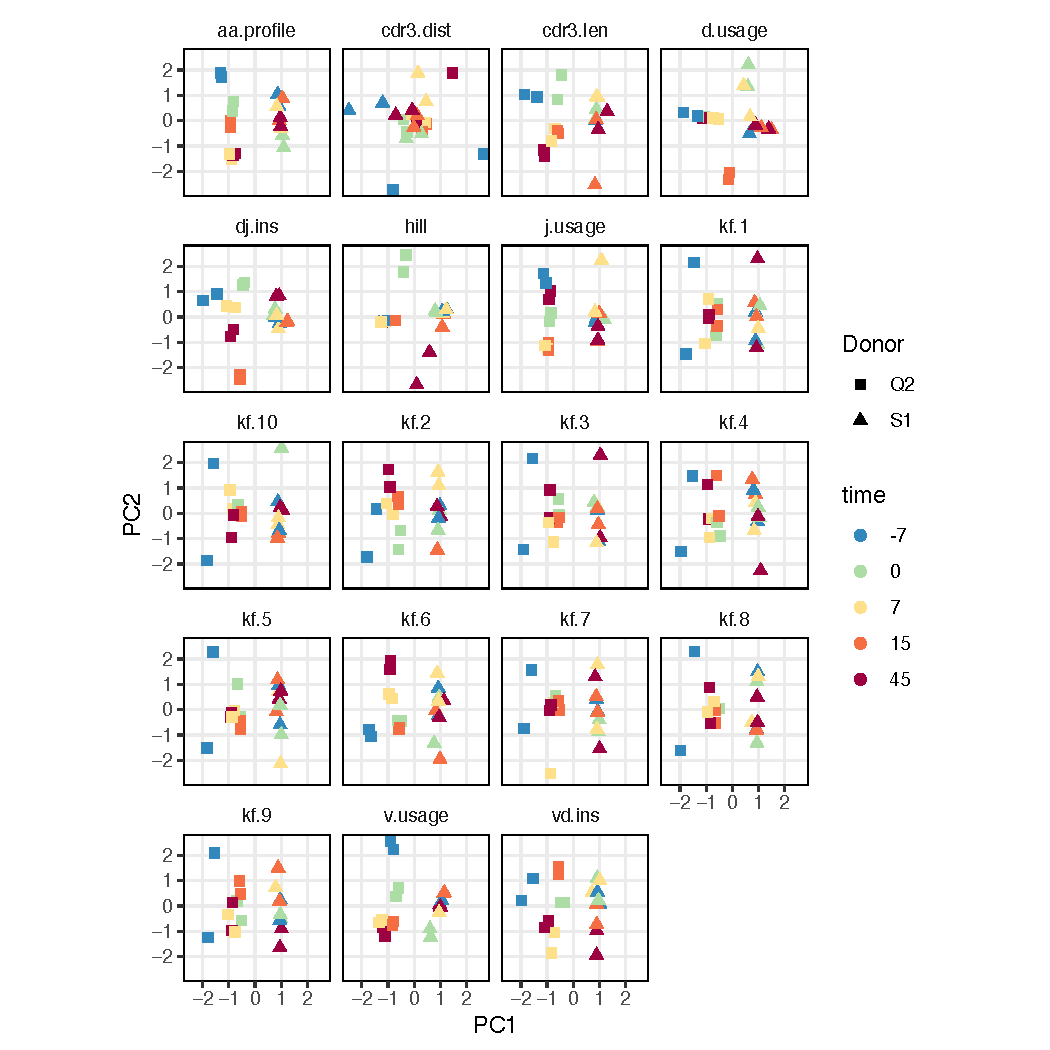
\includegraphics[width=\linewidth]{Figures/tcr_pca.pdf}
    \caption{Plots of summary divergence MDS coordinates for the Pogorelyy (2018) data, grouped by donor and timepoint}
    \label{fig:TCR_MDS}
\end{figure}
We see that for almost all summaries, these points cluster according to donor identity, with the CDR3 pairwise distance distribution being the only summary that does not decisively cluster by donor.
%EM I'm not totally convinced that the cross is more than just random noise...
The D gene usage distribution has more unusual cross-like pattern, whose structure is more difficult to assess.
Other summaries, such as the CDR3 pairwise distance distribution and Hill numbers, yield little to no signal.
Moreover, there does seem to be signal induced by donor-timepoint interactions, although the tightness of clustering varies by summary, with some summaries (e.g. DJ insertion length distribution) being tightly clustered by a given donor/timepoint value and some summaries (e.g. Kidera factor 4) not obviously clustering by donor/timepoint.
Although these patterns would require further exploration in a particular research context, there seem to be interesting dynamics underlying \texttt{sumrep} divergences when datasets are stratified by covariates.


\subsection*{Orthogonality analysis}
Due to the large number of summary statistics supported by \texttt{sumrep}, some of which are inter-correlated, we sought an approach to identify a set of maximally-informative statistics that are orthogonal by some measure.
To address this, we employed an $\ell_1$-regularized (a.k.a. lasso) multinomial regression by treating the summaries as covariates and dataset identity as the response.
The basic idea is that this regression method cuts out all but a few predictor variables to find a smaller collection of informative summary statistics.
In $\ell_1$ regression, a coefficient is ``allowed'' to be nonzero only when the lasso deems it a relatively meaningful predictor.
As the regularization parameter $\lambda$ is decreased, more and more coefficients branch become nonzero, leading to a natural ordering of summaries as the order in which their coefficient ``branches off'' from zero.
Since $\ell_1$ multinomial regression outputs a separate coefficient vector $\boldsymbol \beta$ for each response value, we aggregate by taking medians of each dataset-specific lasso ordering for each summary.
Detailed pseudocode is provided in Algorithm \ref{alg:Lasso}.
\begin{algorithm}
    \caption{Rank summary statistics by informativeness\\
        \textbf{Input:} annotations datasets $d_1, \dotsc, d_D$, sequence-level summaries $\mathbf s(\cdot) = [s_1(\cdot), \dotsc, s_S(\cdot)]$, lasso parameters $\lambda_1, \dotsc, \lambda_\Lambda$ \\
        \textbf{Output:} A vector of ranks for the summaries }
    \label{alg:Lasso}
    \begin{algorithmic}
   		\For{$d = d_1, \dotsc, d_D$}:
			\State $\mathbf X_d \gets [\mathbf s(d_1), \dotsc, \mathbf s(d_D)]$
    	\EndFor
		\State $\mathbf X \gets \begin{bmatrix}
			 \mathbf X_1 \\ \vdots \\ \mathbf X_D 
			 \end{bmatrix}$
		\State $\mathbf y \gets \begin{bmatrix}
			\text{rep}(1, \text{rows}(d_1))^\mathsf{T}
			\\ \vdots \\
			\text{rep}(D, \text{rows}(d_D))^\mathsf{T}
		\end{bmatrix}$
        \For{$\lambda = 1, \dotsc, \lambda_\Lambda$}:
        	\State $(\boldsymbol \beta_1^\lambda, \dotsc, \boldsymbol \beta_D^\lambda) \gets \text{MultinomialLasso}(\mathbf X, \mathbf y; \lambda)$
        \EndFor
        \For{$d = 1, \dotsc, D$}:
        	\For{$s = 1, \dotsc, S$}:
				\State $t_{d, s} \gets 
				\min\left( \min \left\{ \lambda_1 \le \lambda \le \lambda_\Lambda: \beta_{d, s}^\lambda > 0 \; 
					\forall t > \lambda \right\},
					\infty \right)$
			\EndFor
        \EndFor
        \State $\mathbf T = (t_{d, s})_{1 \le d \le D, 1 \le s \le S}$
        \State $\text{scores} = \text{rank}\left( \median_{s_1}(\mathbf T),
        	 \dotsc, \median_{s_S}(\mathbf T) \right)$
       \State \Return scores
    \end{algorithmic}
\end{algorithm}

This approach only works for sequence-level summaries $s \in \mathbb{R}^n$ for datasets of $n$ sequences in order to form a well-defined design matrix $\mathbf X \in \mathbb{R}^{\left(\sum_{d=1}^D \text{rows}(d) \right) \times S}$.
For example, it is unclear how to incorporate the pairwise distance distribution, which is not a sequence-level summary, as a covariate, since this summary in general yields a column of a larger length than the number of sequences. 
Still, as most summaries considered above can be applied at the sequence level, this method greatly reduces the number of summaries the user needs to examine.

Figure \ref{fig:IgorLasso} displays the results of applying Algorithm~\ref{alg:Lasso} to the six \igor-annotated TRB datasets from \cite{Britanova2016-iw}.
We see that deletion lengths comprise four of the top five summaries, with insertion lengths, CDR3 length, and various physiochemical junction properties scattered over the remaining positions.
There appears to be high variability throughout the range of rankings, with the bottom three statistics all having a ranking of one for at least one coefficient vector.
\begin{figure}
    \begin{subfigure}{\linewidth}
    	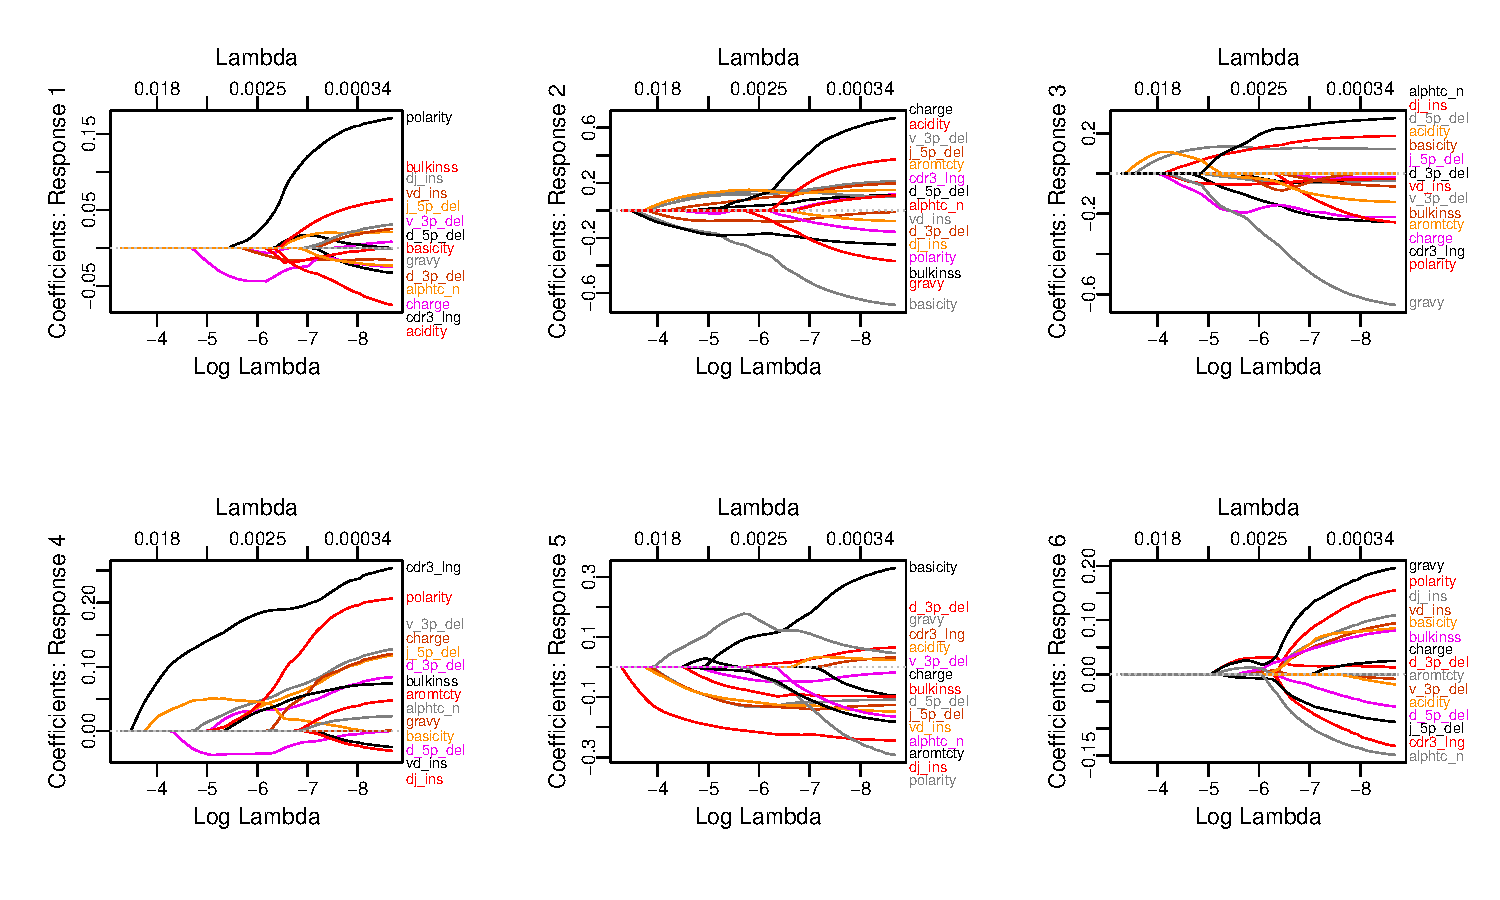
\includegraphics[width=\linewidth]{Figures/Lasso/igor_lasso_paths.pdf}
		\caption{Lasso paths of summary coefficients for each of the six datasets.}
    \end{subfigure}
    \begin{subfigure}{\linewidth}
    	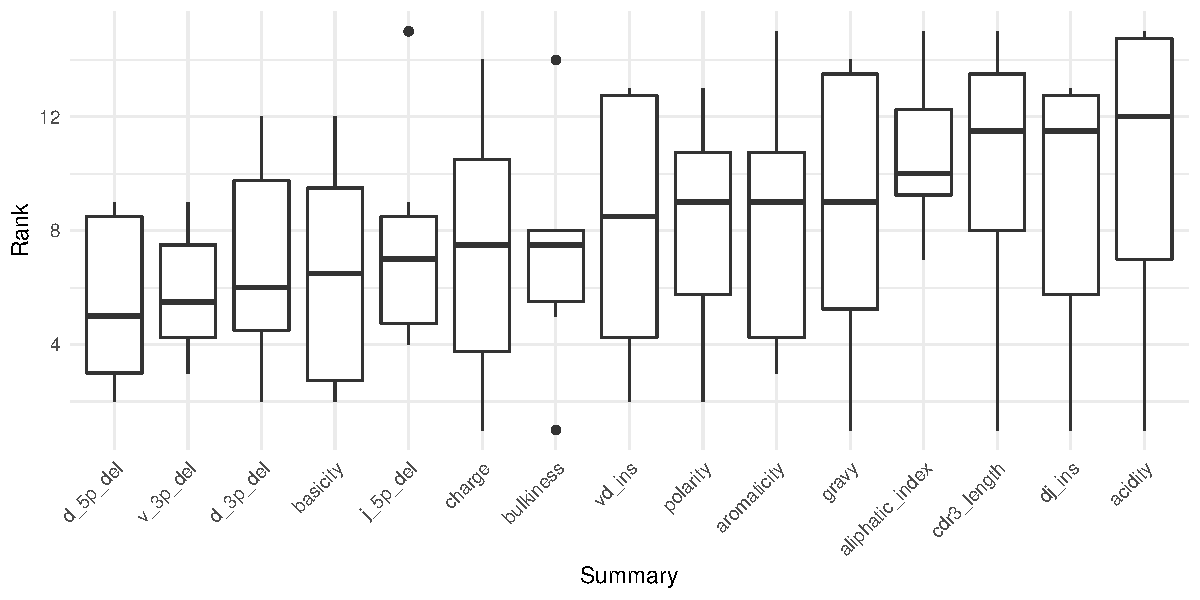
\includegraphics[width=\linewidth]{Figures/Lasso/igor_lasso_scores.pdf}
		\caption{Boxplots of summary rank values taken over each dataset.}
    \end{subfigure}
    \caption{Results of applying Algorithm~\ref{alg:Lasso} to the six \igor\-annotated TRB datasets from Britanova (2016).}
    \label{fig:IgorLasso}
\end{figure}

Figure \ref{fig:PartisLasso} displays the results of applying Algorithm~\ref{alg:Lasso} to the six \partis-annotated TRB datasets from \cite{Gupta2017-ve}.
We see that deletion lengths, insertion lengths, and CDR3 length comprise the top six summaries, with physiochemical junction properties mostly in the bottom half of rankings.
In contrast to the TCR result, there appears to be less overall variability throughout the range of rankings, with variability highest for the moderate ranking positions and notably lower for the top and bottom positions.

\begin{figure}
    \begin{subfigure}{\linewidth}
    	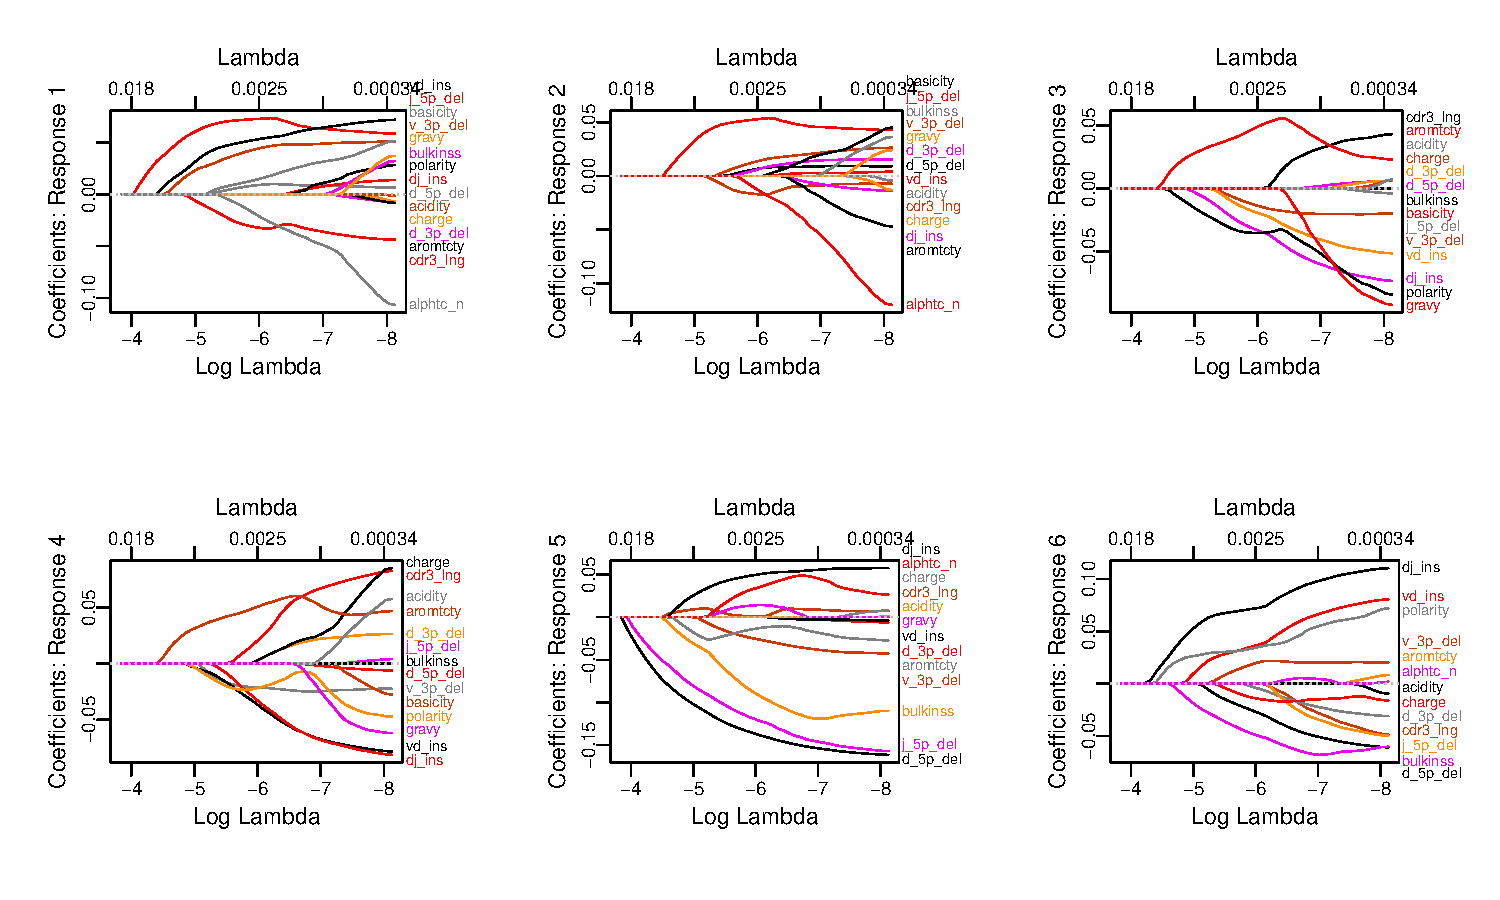
\includegraphics[width=\linewidth]{Figures/Lasso/partis_lasso_paths.pdf}
		\caption{Lasso paths of summary coefficients for each of the six datasets.}
    \end{subfigure}
    \begin{subfigure}{\linewidth}
    	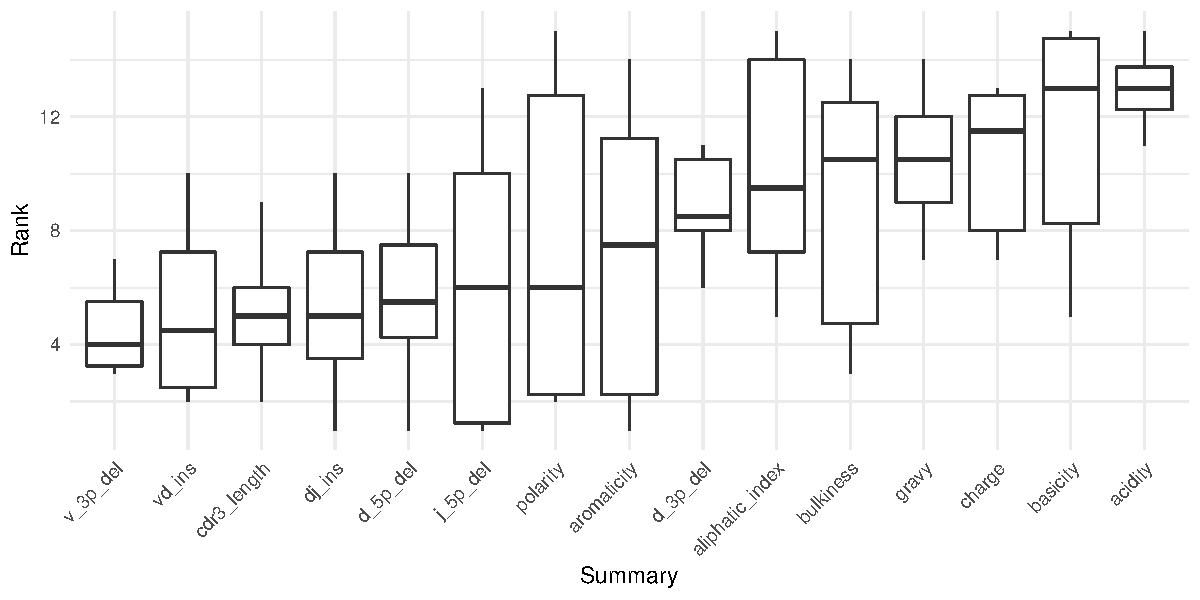
\includegraphics[width=\linewidth]{Figures/Lasso/partis_lasso_scores.pdf}
		\caption{Boxplots of summary rank values taken over each dataset.}
    \end{subfigure}
    \caption{Results of applying Algorithm~\ref{alg:Lasso} to the six \igor-annotated TRB datasets from Gupta (2017).}
    \label{fig:PartisLasso}
\end{figure}

\subsection*{Comparing observations to model simulations per model}
\texttt{sumrep} can be used to validate BCR/TCR generative models, i.e.\ models from which one can generate (simulate) data, through the following approach.
First, given a collection of repertoire datasets, infer model parameters using software based on the given model for each repertoire, and use these parameters to generate corresponding simulated datasets.
Next, use \texttt{sumrep} to compute each summary statistic listed in Table~\ref{tab:SummaryStatistics} for each dataset, and compare these summaries between each pair of datasets.
Then, calculate a score of how well the software's simulation replicates a given summary based on how small the divergences of observed/simulated dataset pairs are compared to divergences between arbitrary observed/observed or simulated/simulated pairs.

Applying this methodology using many datasets should give a clear view of which characteristics the model captures well, as well as areas for improvement.
As described in the introduction, we are motivated to do this because models are often benchmarked on simulated data, and it is important to understand discrepancies between simulated and observed data in order to properly interpret and extrapolate benchmarking results.
We emphasize that validating the model in this way is different than the usual means of benchmarking model performance-- rather than benchmarking the inferential results of the model, we benchmark the model's ability to generate realistic sequences.

We illustrate this approach with two case studies:
an analysis of IGoR \cite{Marcou2018-du} applied to TRB sequences, and an analysis of \texttt{partis}\cite{Ralph2016-nw, Ralph2016-iz} simulations applied to IgH sequences.
Both tools are applied to separate sets of experimental repertoires, yielding model-based annotations for each repertoire, as well as simulated datasets from the inferred model parameters for each experimental set.
Relevant scores of each summary for each tool are computed using each observed and simulated dataset.

%EM Agreed here!
%BJO - TODO: Add quick summaries of the IGoR and partis analyses as summarized form the Methods subsections

\subsection*{Assessing summary statistic replication for \texttt{igor}}
We apply the methodology discussed in the previous section to TRB sequences from \cite{Britanova2016-iw}.
The full study sequenced experimental TRB repertoires from various donors across the lifespan, although we only examine six datasets here as discussed in the materials section.
Figure~\ref{fig:IgorFreqPolys} displays frequency polygons of each summary for each experimental and simulated repertoire, and Figure~\ref{fig:IgorECDFs} displays the corresponding empirical cdfs.
\begin{figure}
    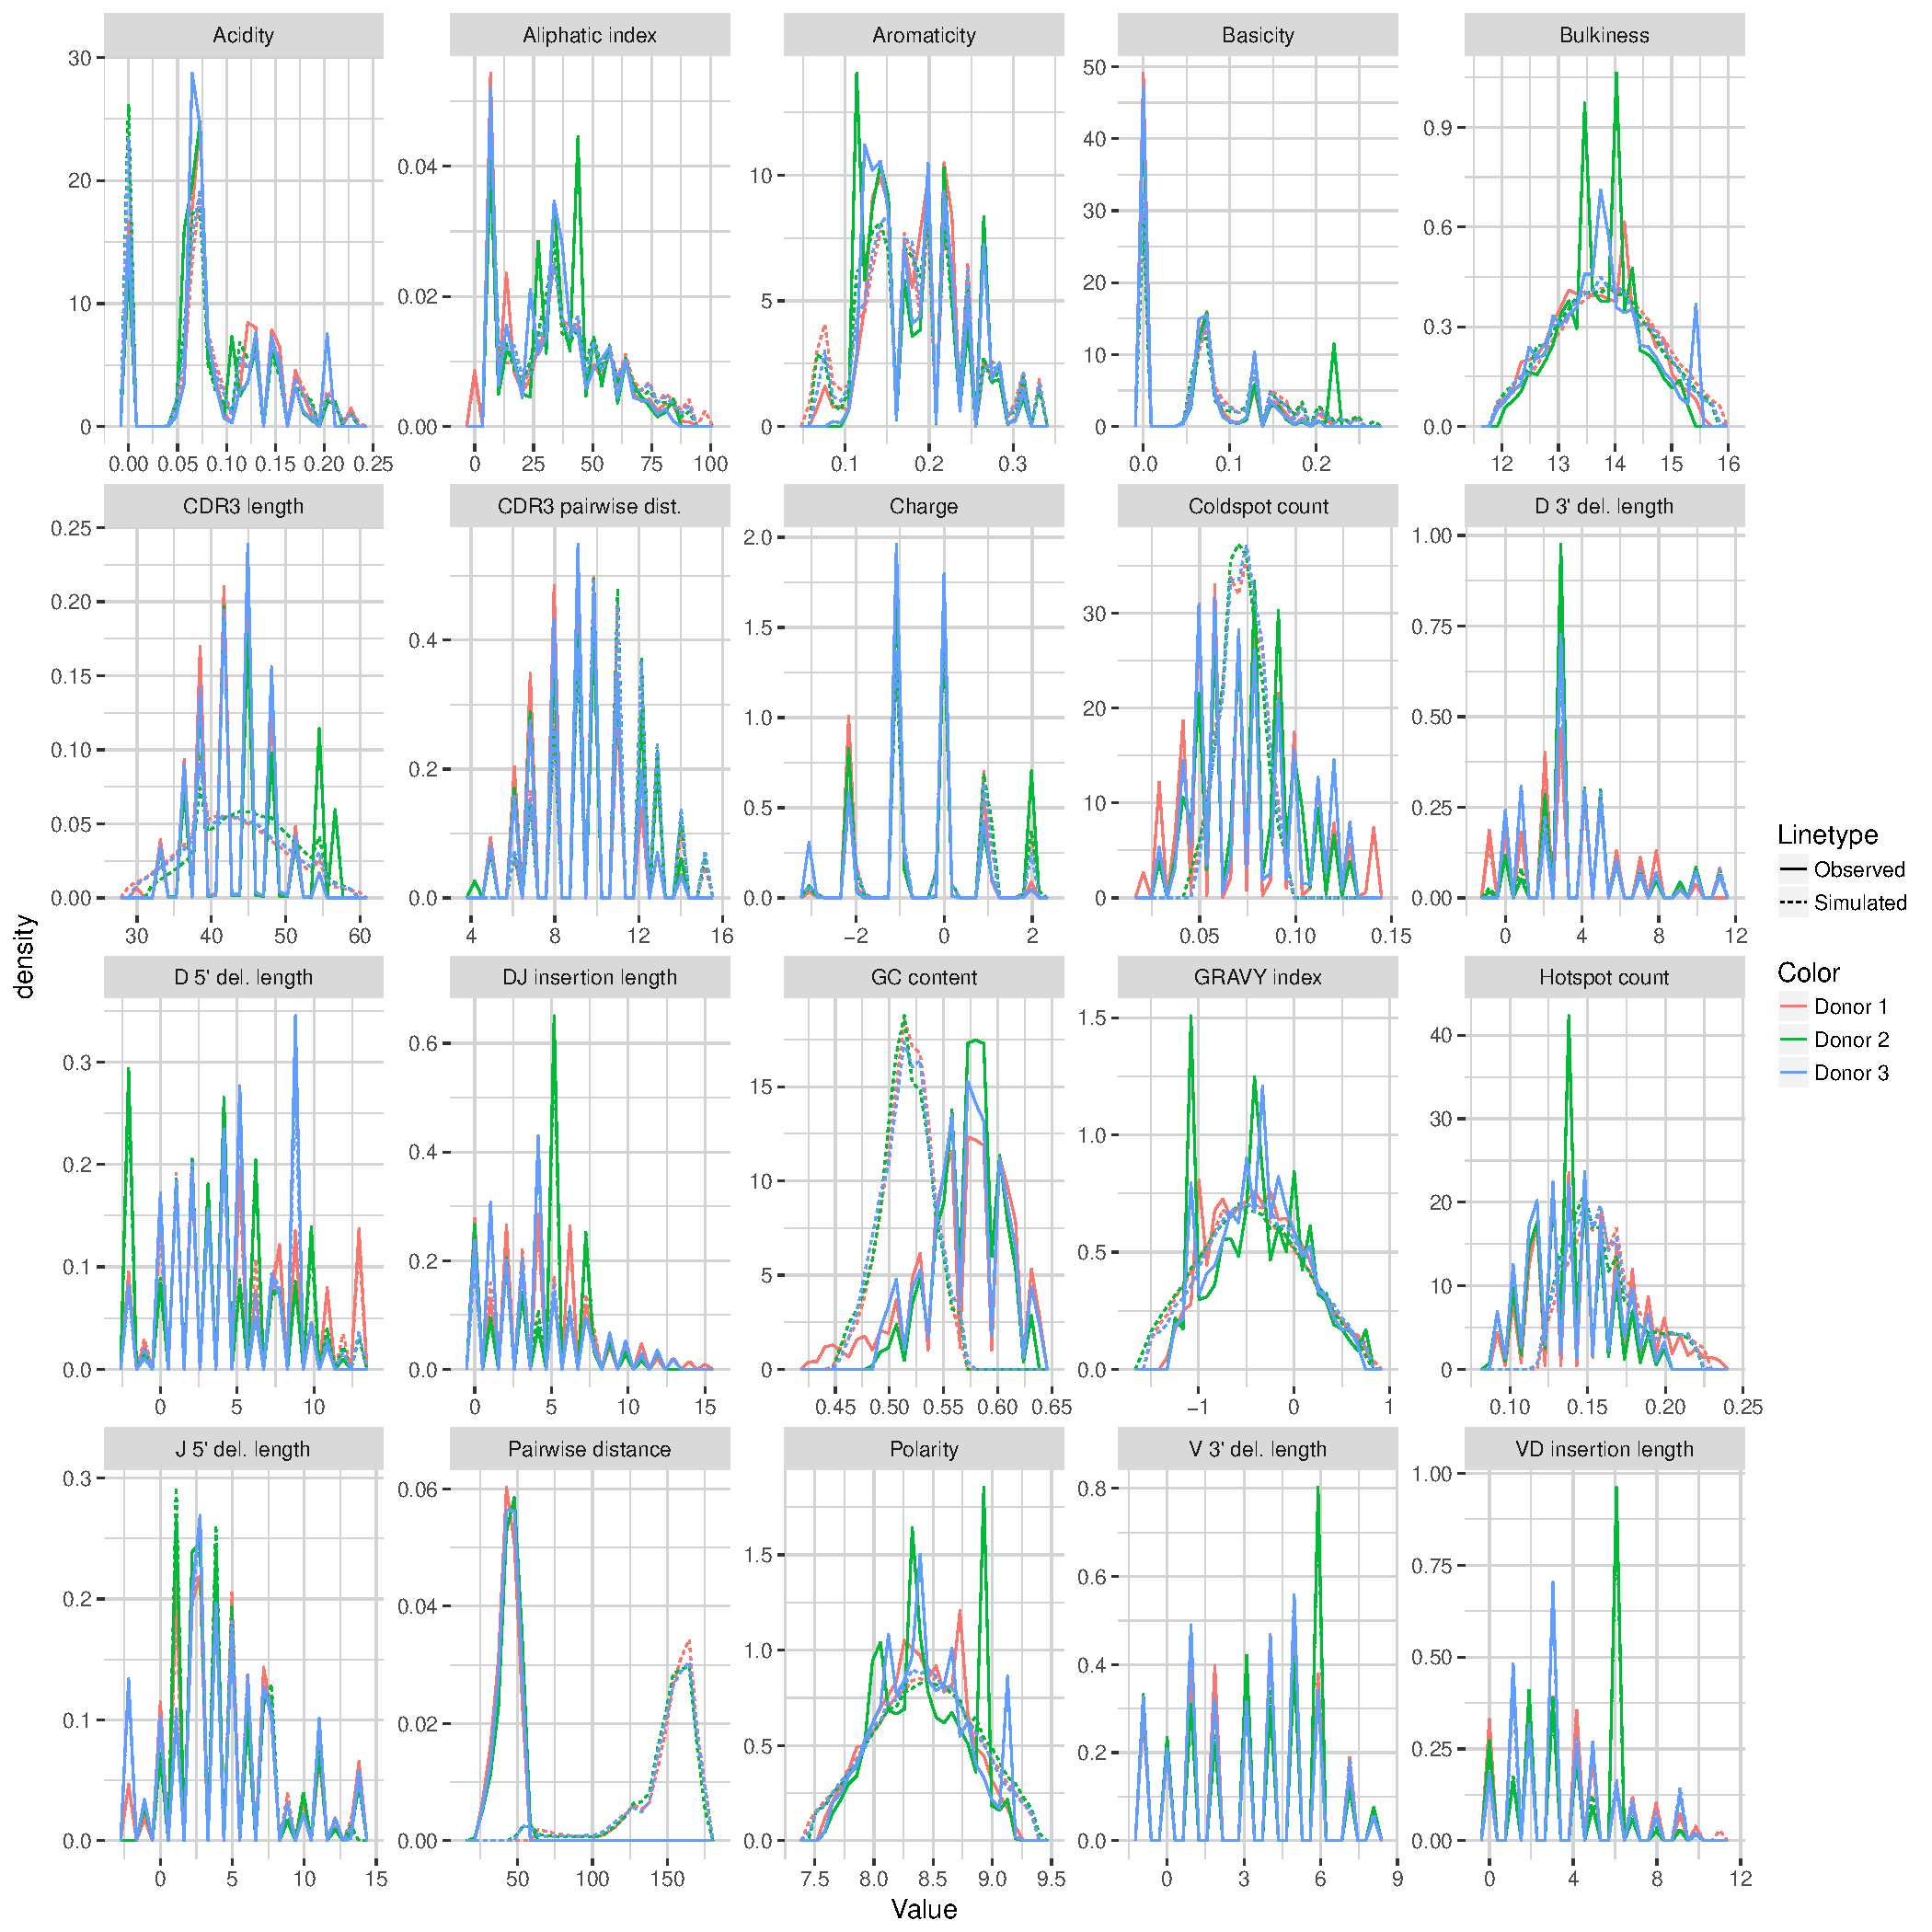
\includegraphics[width=\linewidth]{Figures/IgorScores/igor_freqpoly.pdf}
    \caption{Frequency polygon plots of each univariate summary distribution for the IGoR datasets.}
    \label{fig:IgorFreqPolys}
\end{figure}

\begin{figure}
    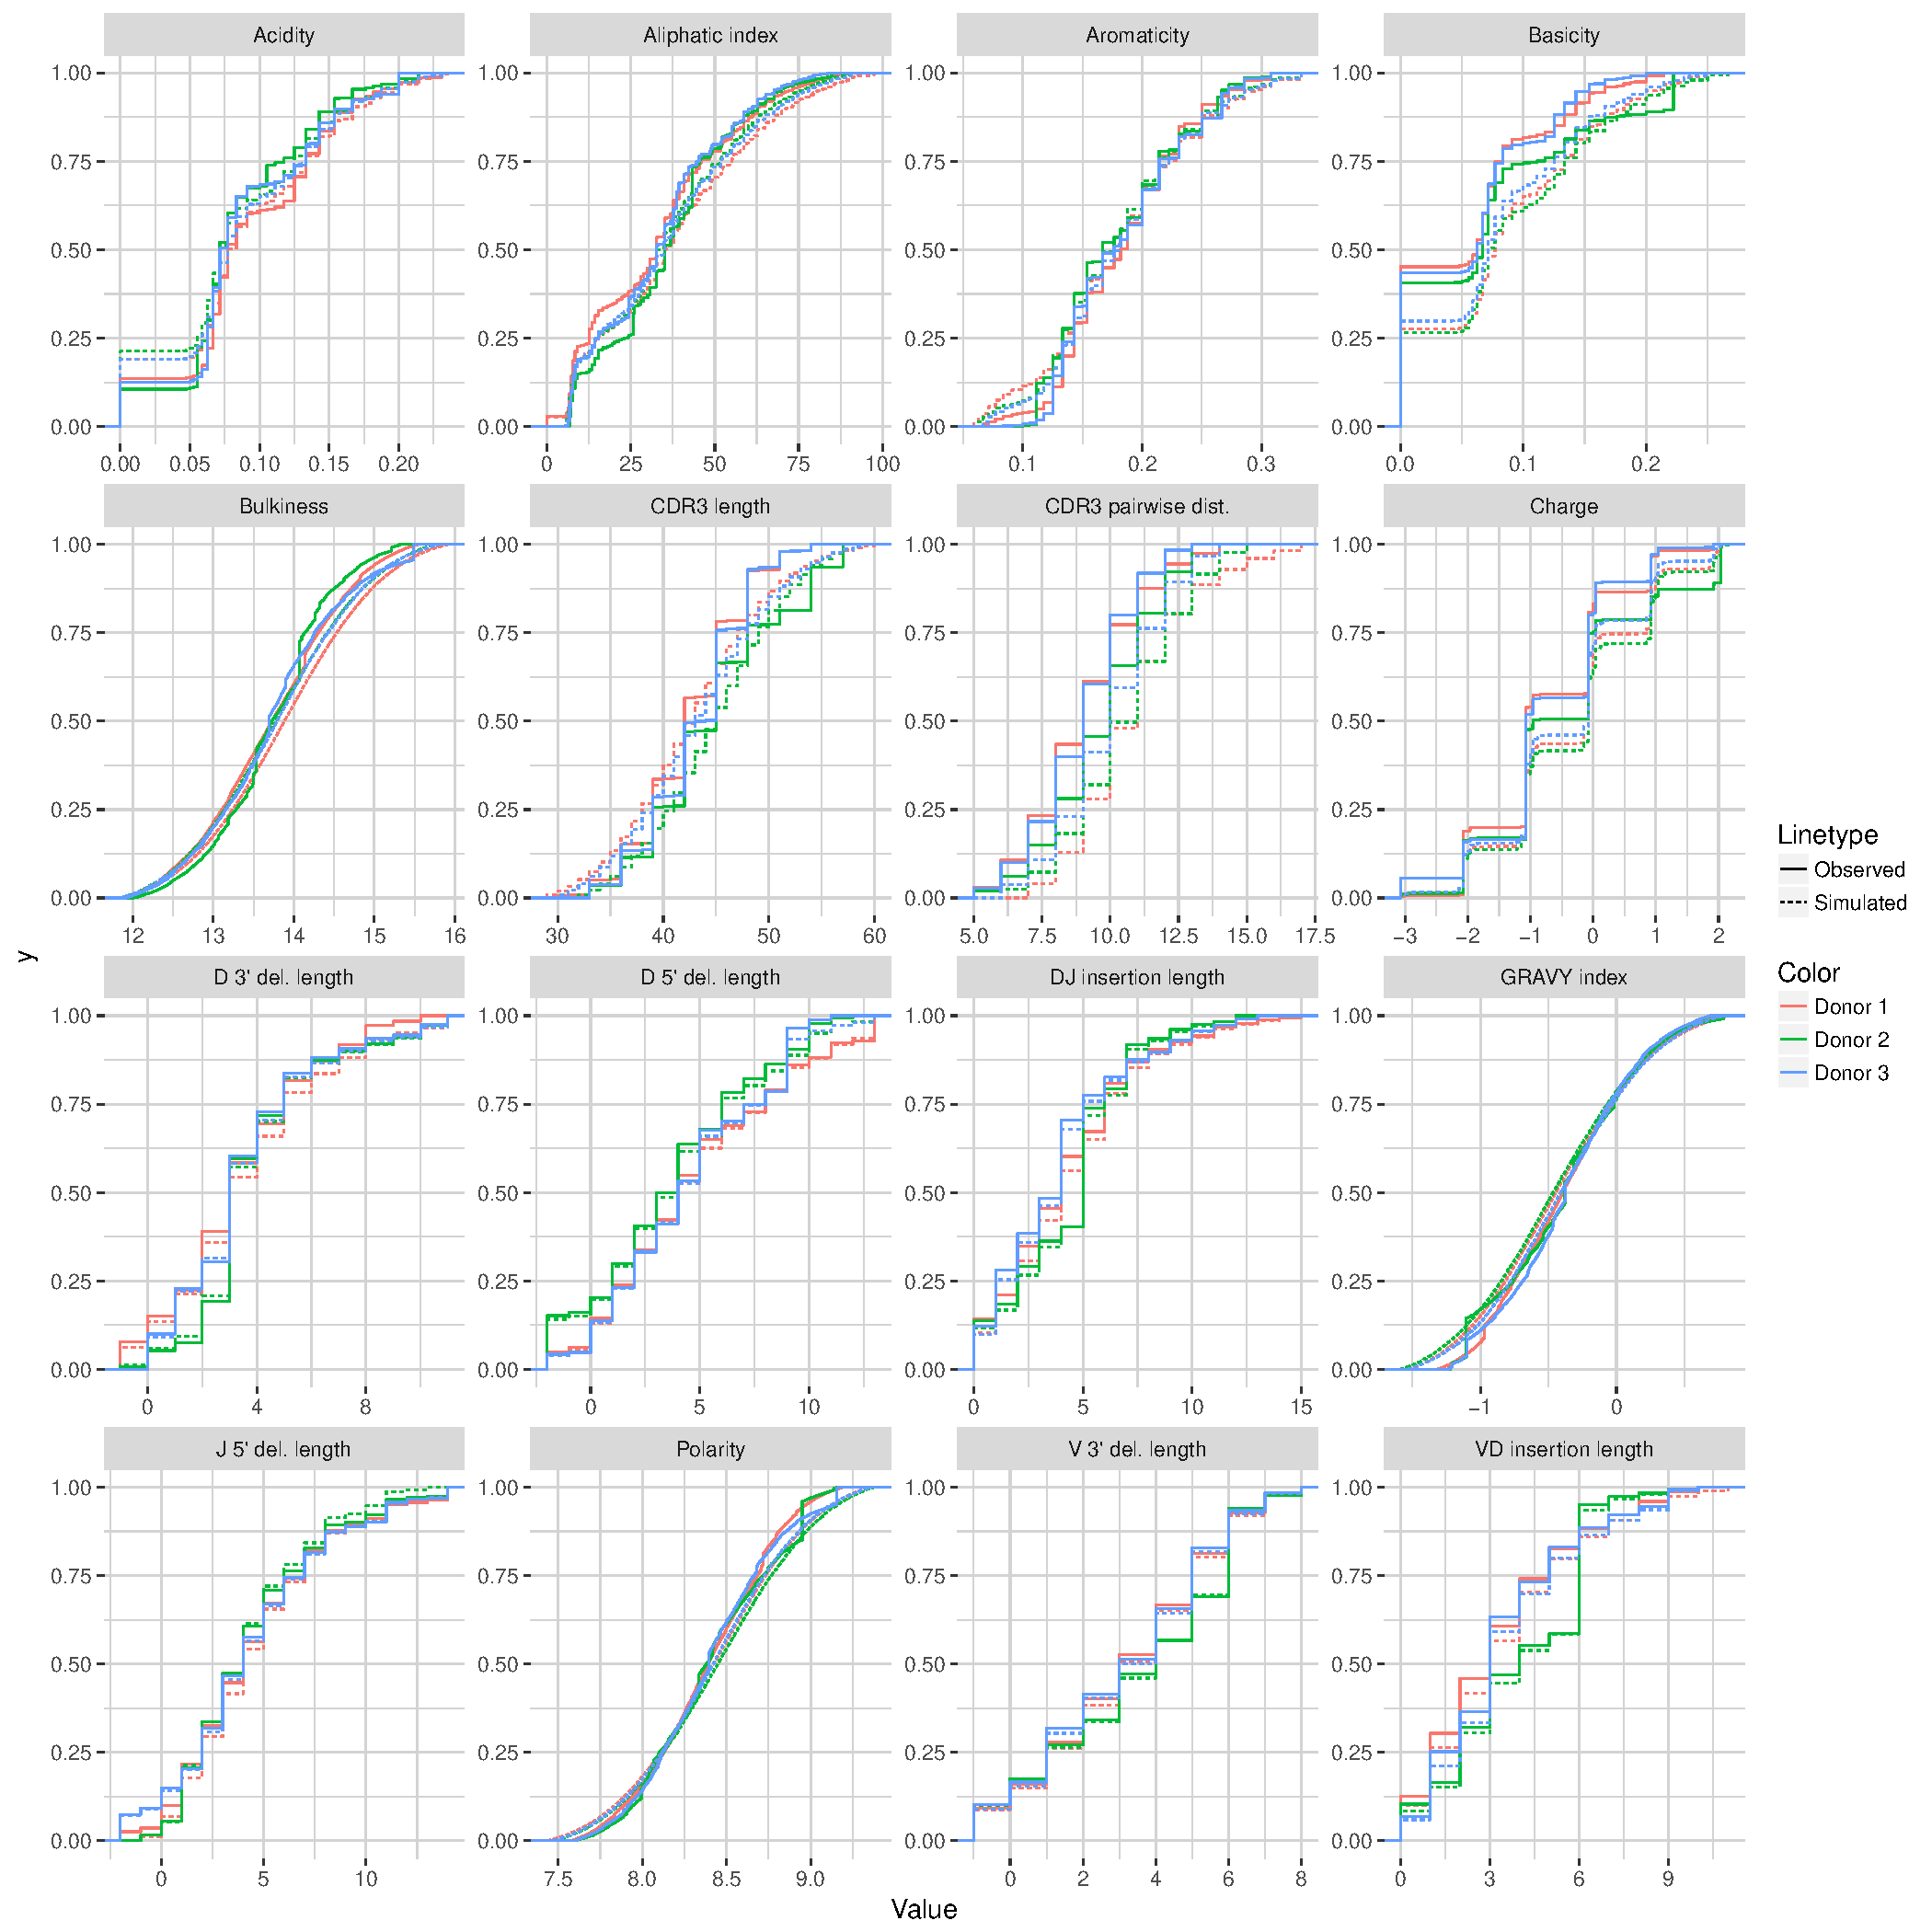
\includegraphics[width=\linewidth]{Figures/IgorScores/igor_ecdf.pdf}
    \caption{Empirical cumulative distribution function plots of each univariate summary distribution for the IGoR datasets.}
    \label{fig:IgorECDFs}
\end{figure}


Figure~\ref{fig:ObsScoresTCR} displays the observation-based summary scores for the six TRB datasets based on \igor\ simulations.
We exclude \texttt{sequence\_alignment}-based summaries such as GC content and pairwise distance distributions since they are likely compounded by differences in the read lengths of the query sequences versus the full variable region nucleotide sequences of the simulations, and IGoR does not currently have an option to output the full variable region nucleotide sequences for experimental reads.
\begin{figure}
	\begin{subfigure}{\textwidth}
    	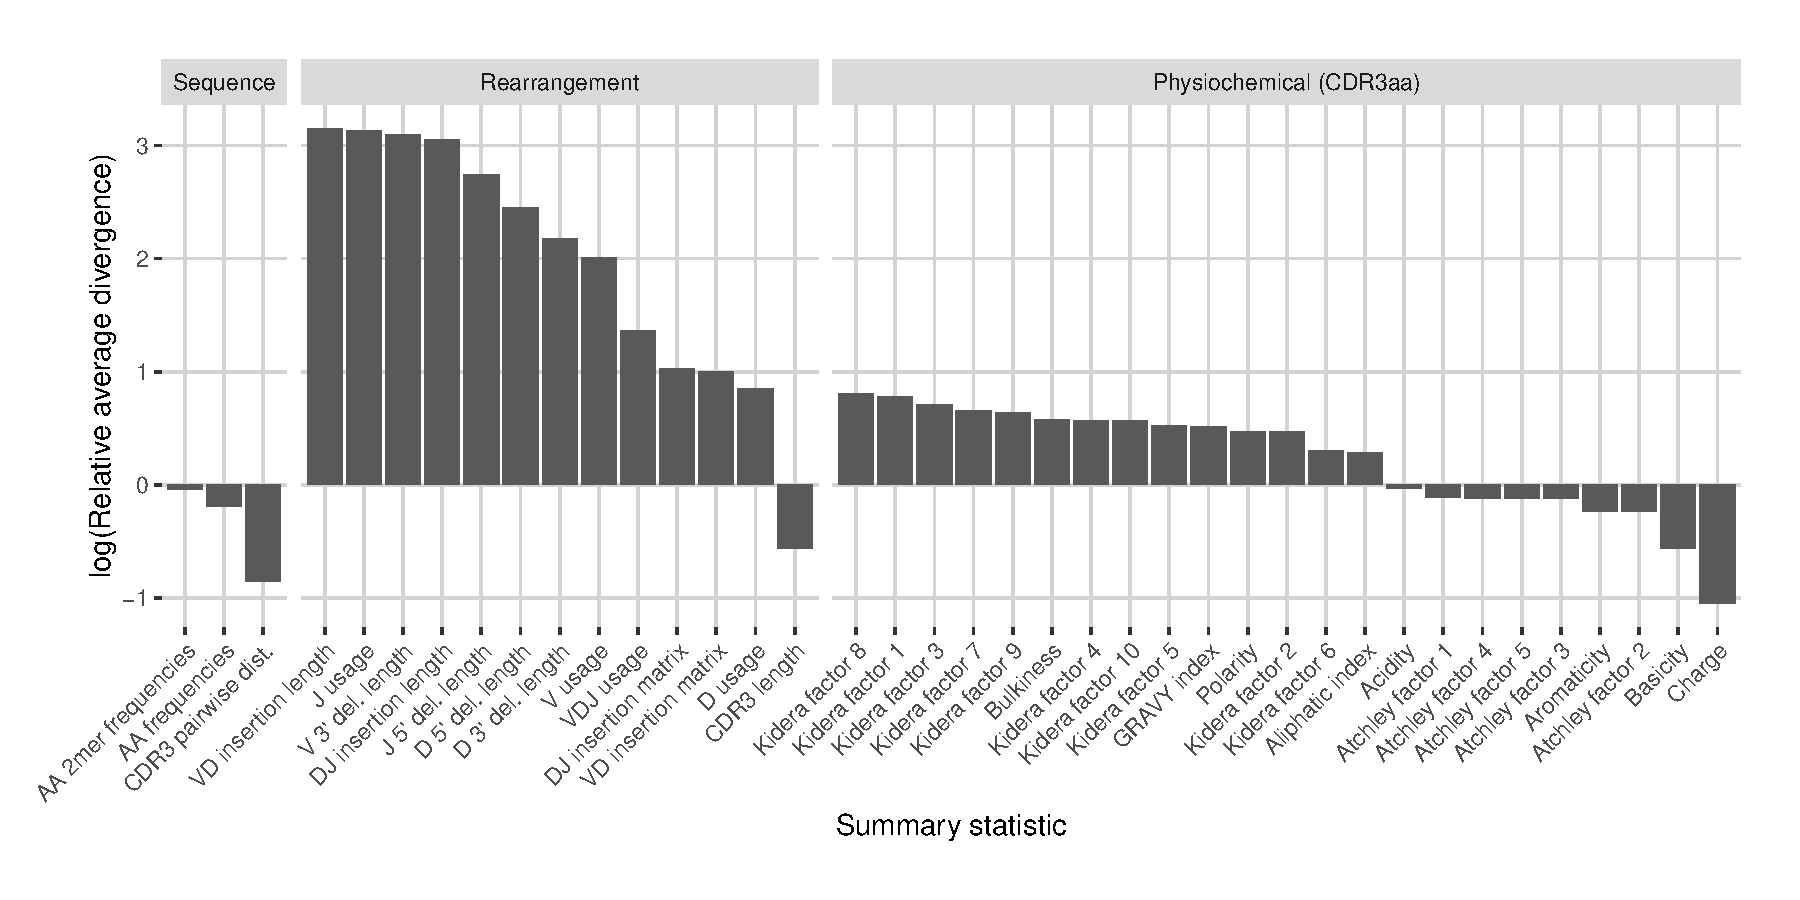
\includegraphics[width=\linewidth]{Figures/IgorScores/obs_score_plot.pdf}
    	\caption{$\text{score}_\text{obs}$ values for each statistic.
        %EM Seems like one more phrase of explanation would help make this figure easier to interpret. It's functional(?) TCR data (and partis is BCR data...)
        %BJO I added a caption for the full figure and elaborated -- would you like more explanation?
        }
    	\label{fig:ObsScoresTCR}
	\end{subfigure}
	\begin{subfigure}{\textwidth}
    	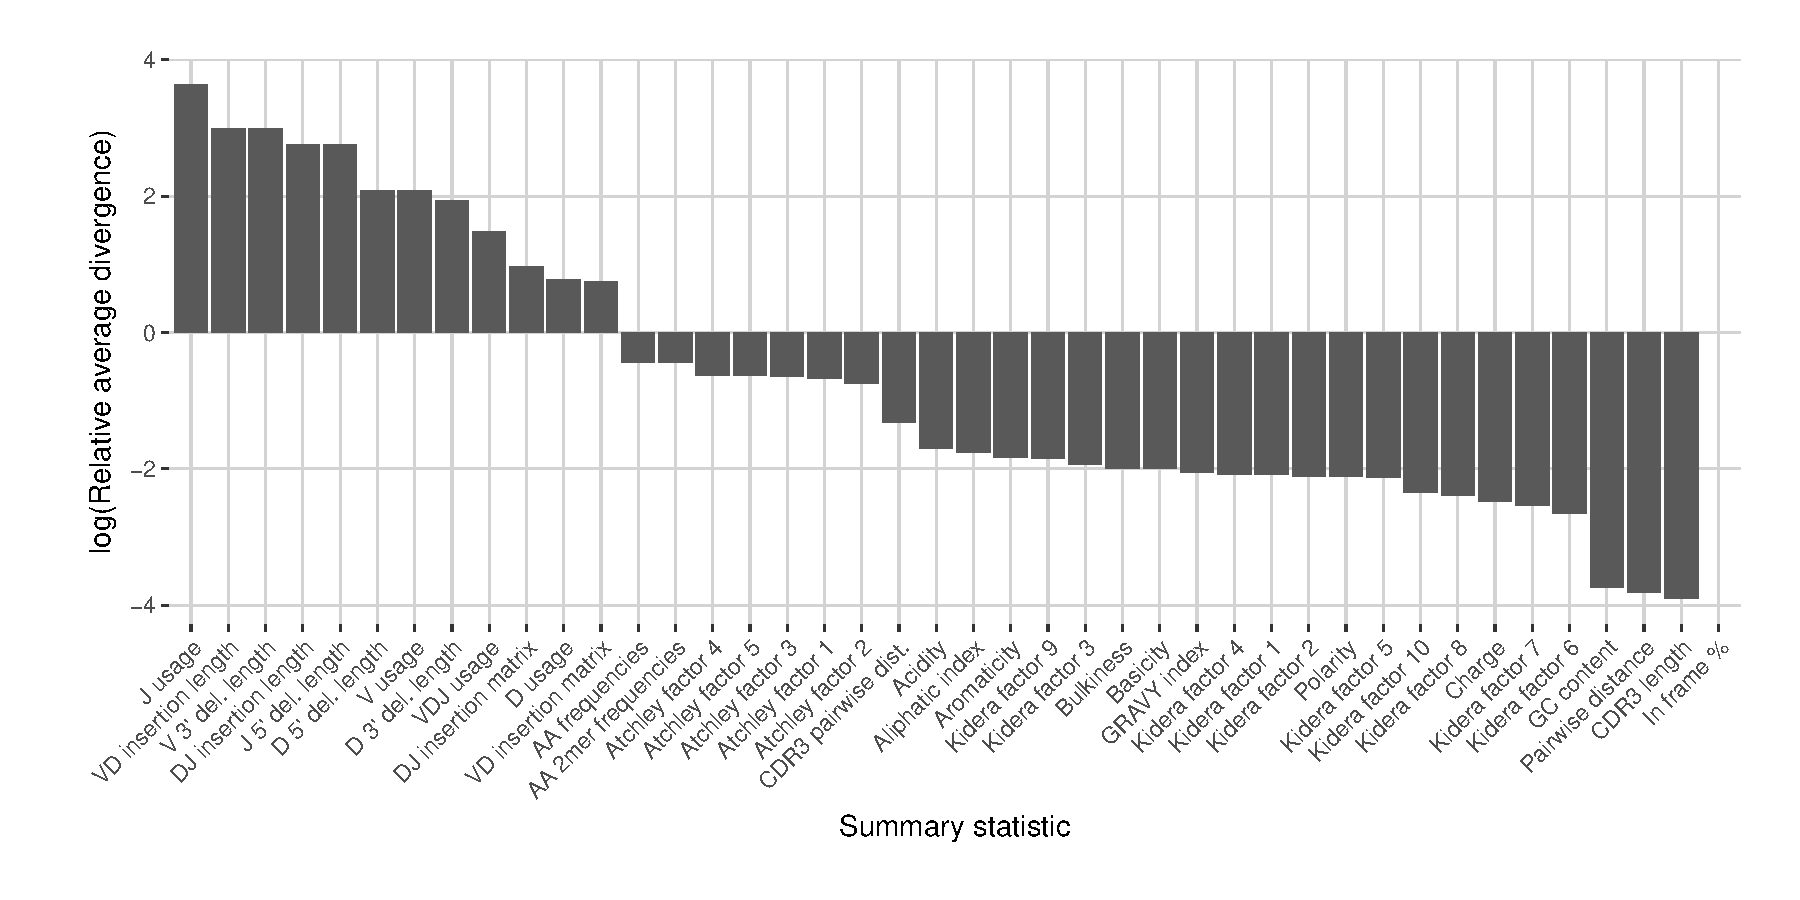
\includegraphics[width=\linewidth]{Figures/IgorScores/sim_score_plot.pdf}
    	\caption{$\text{score}_\text{sim}$ values for each statistic.
    	}
    	\label{fig:SimScoresTCR}
	\end{subfigure}
	\caption{Summary scores, denoted as "log(Relative average divergence)" due to the form of Equations \ref{eq:ScoreObs} and \ref{eq:ScoreSim}, for each statistic in the \igor\ model validation experiment. For both cases, a high score indicates a well-replicated statistic by the simulations with respect to their corresponding experimental repertoires of functional TRB sequences.}
\end{figure}
It is seen that IGoR simulations are able to recapitulate gene usage statistics of an empirical repertoire very well, with J gene usage frequency being the most accurately replicated, followed by various indel length statistics.
V, D, and joing VDJ gene usage are all also well-replicated, as well as both VD and DJ insertion matrices.
The CDR3 length distribution is the least-replicated statistic, although the level of discrepancy is perhaps compounded by training IGoR on both functional and nonfunctional sequences.
Interestingly, the Kidera factors of the junction region are also replicated well, despite CDR3 length being one of the least accurately replicated statistics.
Other junction-based statistics besides Kidera factors range from mildly good to mildly bad replication, with the GRAVY index distribution being the best junction-based statistic (excluding Kidera factors).

Figure~\ref{fig:SimScoresTCR} displays the simulation-based summary scores for the same datasets and simulations.
We still see high scores for gene usage and indel statistics, although now the various Kidera factor and GRAVY index distributions have lower scores.
This suggests that while the average \texttt{igor} simulation yields Kidera factor and GRAVY index distributions that look more like the observed repertoire's distributions than other observed repertoires do, these simulated repertoires still tend to produce similar distributions to each other, as seen in Figure~\ref{fig:IgorFreqPolys}.



\subsection*{Assessing summary statistic replication for \texttt{partis}}
We apply the same methodology to IgH sequences from \cite{Gupta2017-ve} (originally published in \cite{Laserson2014-dx}).
%BJO Actually, I ran this on the 1h/8d pre-vaccination sets, not post-vaccination. Happy to hear objections if anyone would rather I run on post-vaccination sets.
This data consists of longitudinal IgH repertoires of three donors pre- and post-vaccination with influenza; we analyze the one-hour post-vaccination and eight-days post-vaccination repertoires for each donor.
Figure~\ref{fig:PartisFreqPolys} displays frequency polygons of each summary for each experimental and simulated repertoire, and Figure~\ref{fig:PartisECDFs} displays the corresponding empirical cdfs.
\begin{figure}
%EM I think that only one of these should go in the main text, but it's a matter for discussion with the group.
    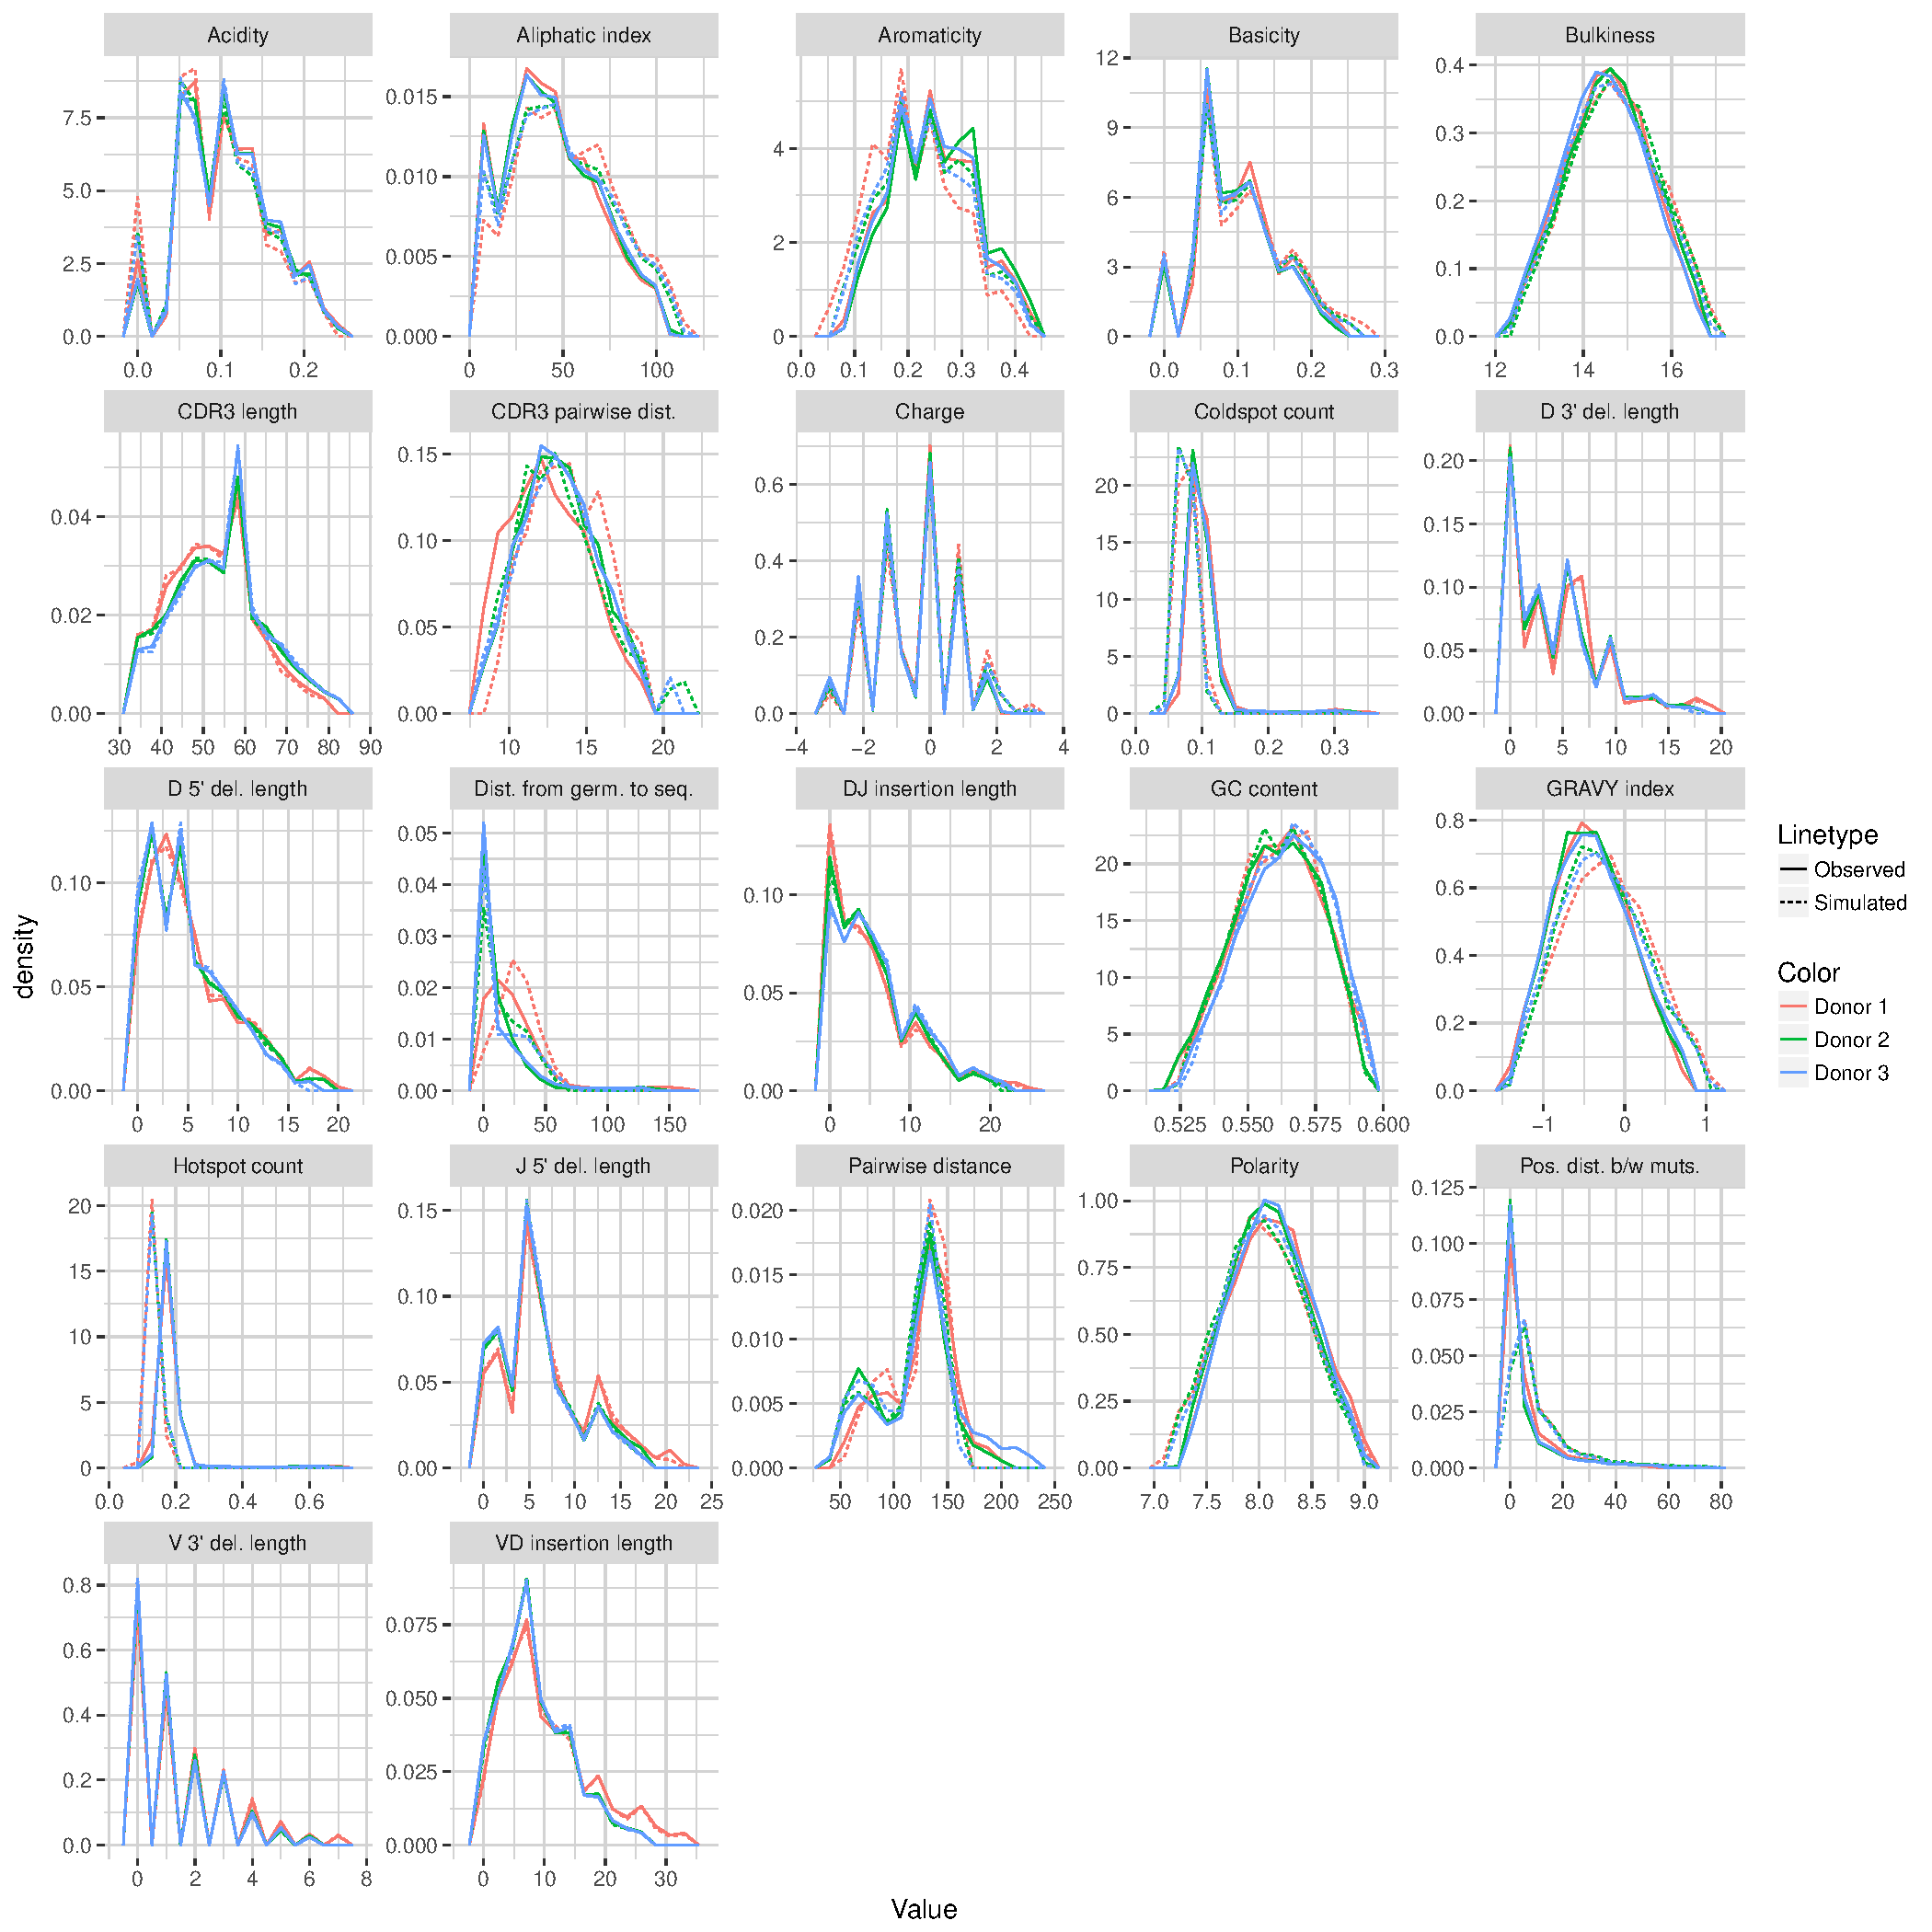
\includegraphics[width=\linewidth]{Figures/PartisScores/partis_freqpoly.pdf}
    \caption{Frequency polygon plots of each univariate summary distribution for the \texttt{p\_f1}, \texttt{p\_f1\_sim}, \texttt{p\_g1}, and \texttt{p\_g1\_sim} datasets.}
    \label{fig:PartisFreqPolys}
\end{figure}

\begin{figure}
    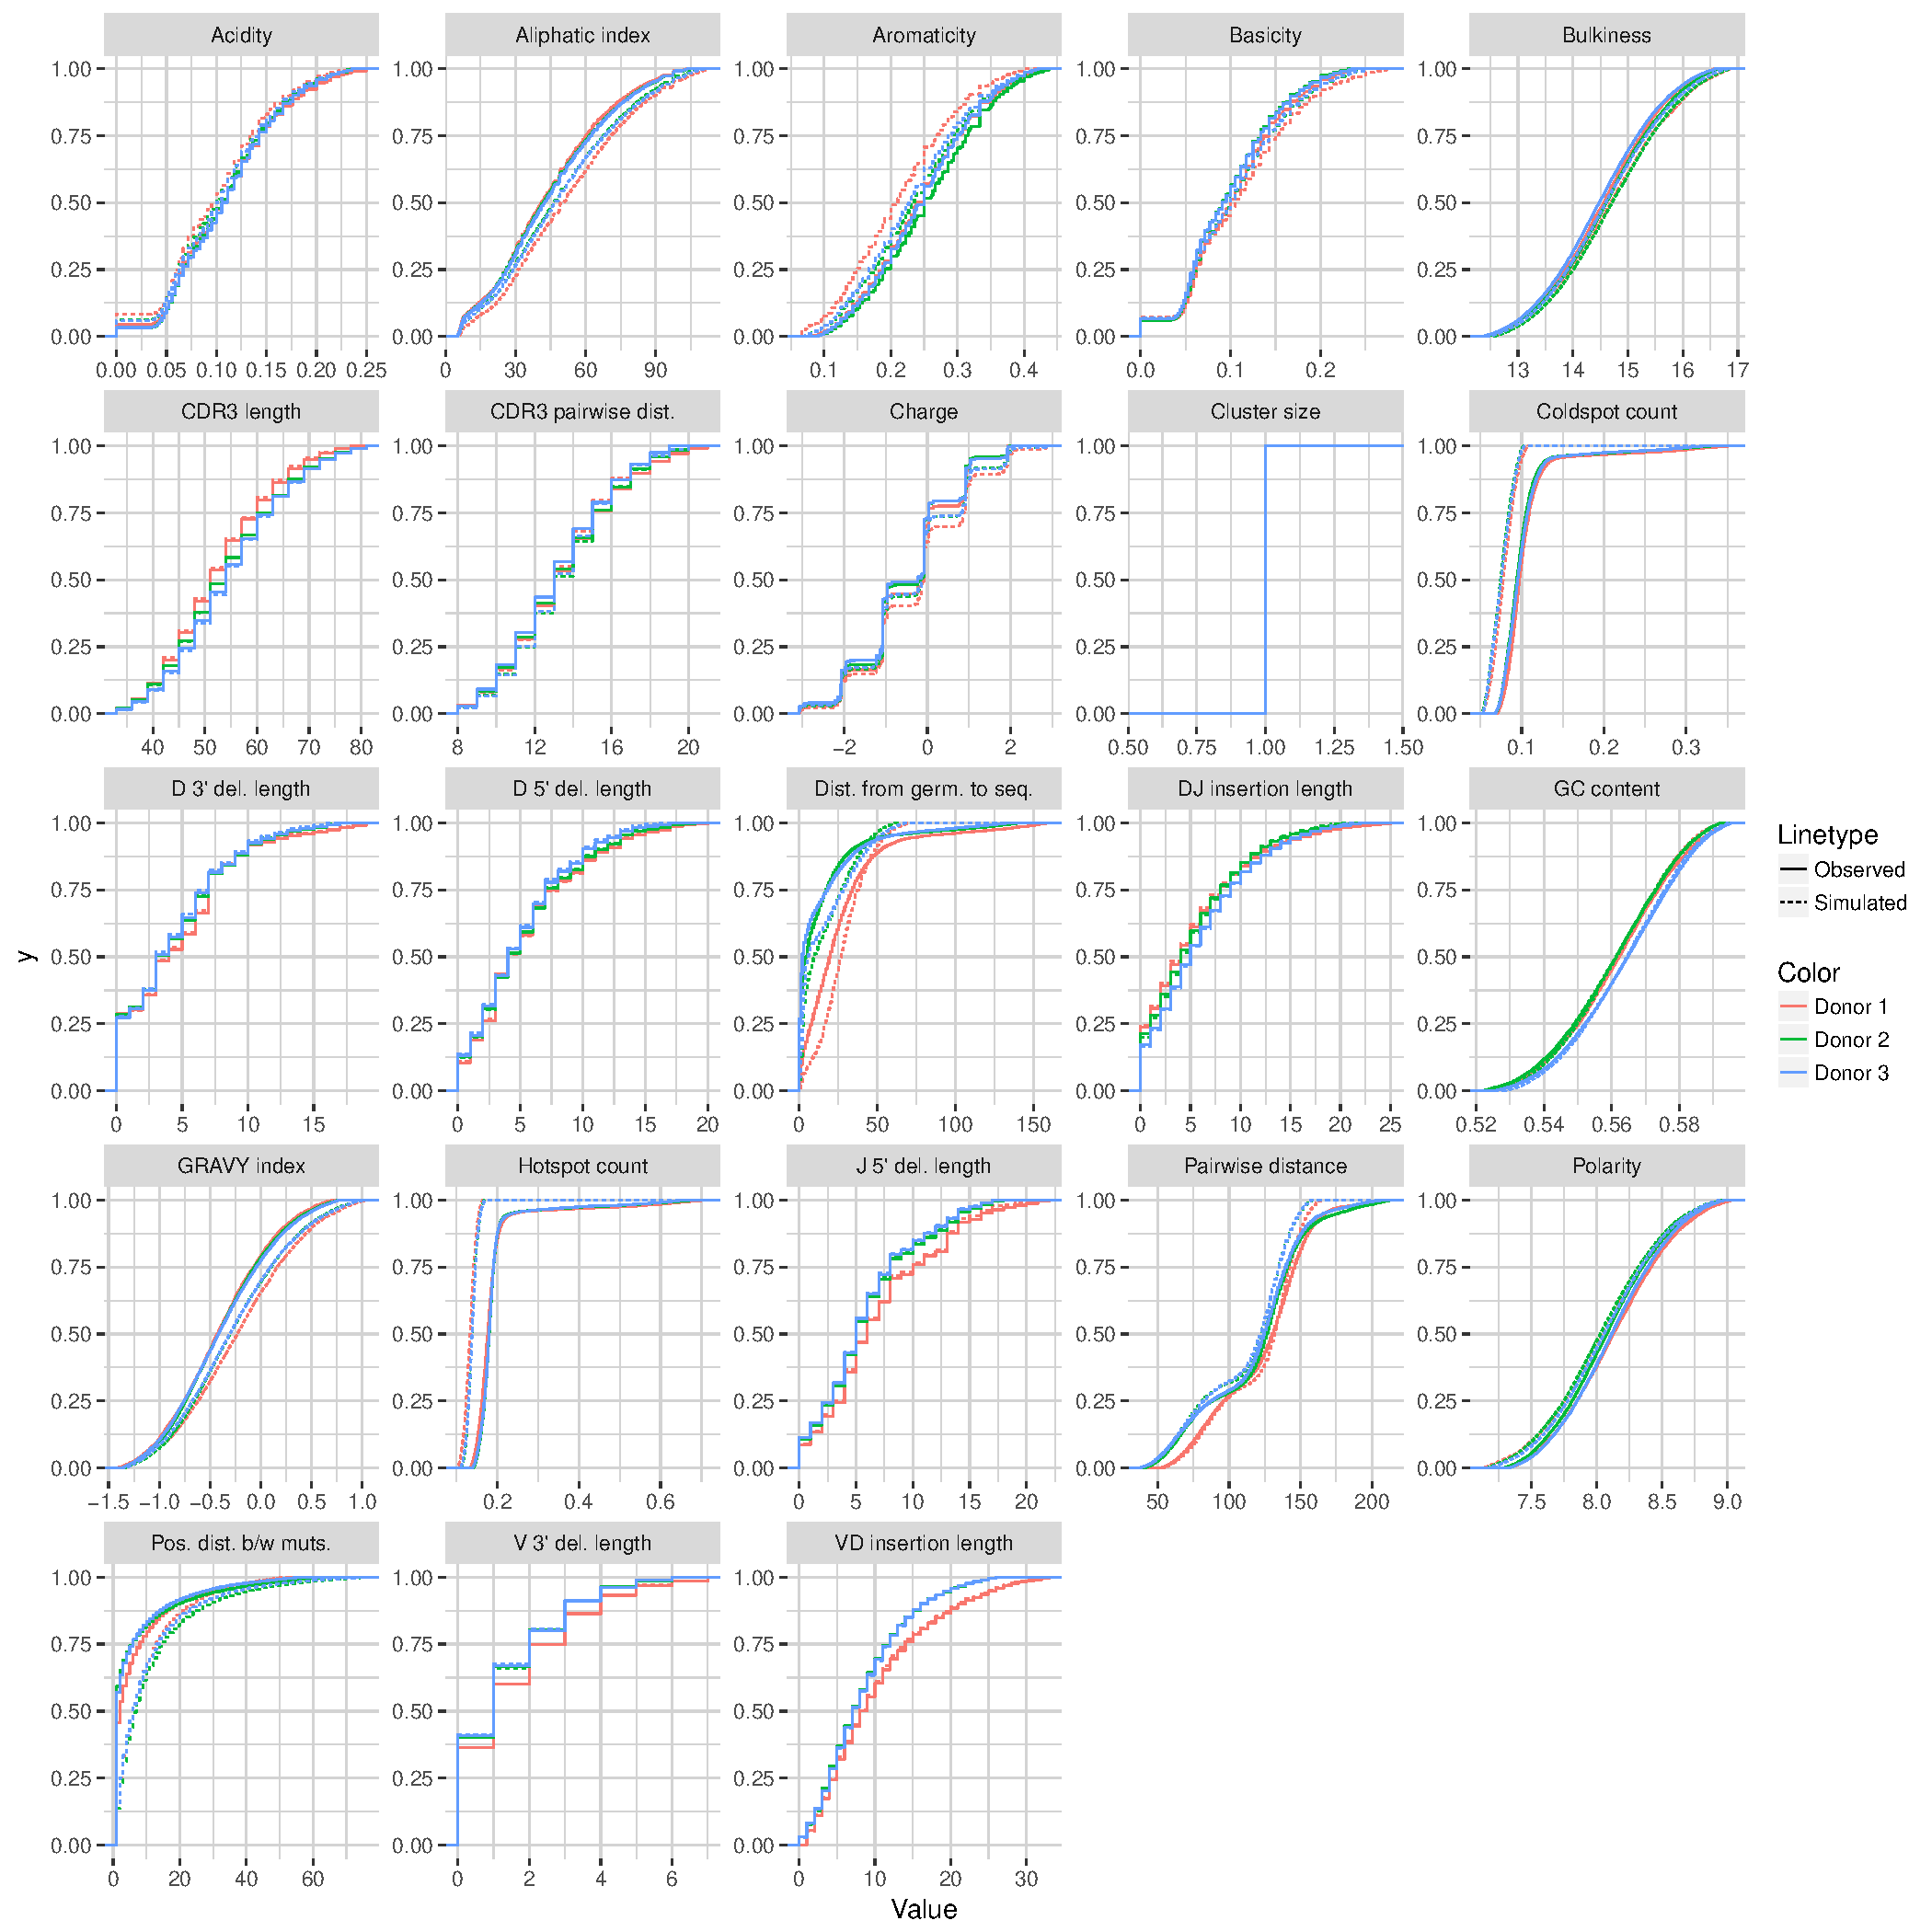
\includegraphics[width=\linewidth]{Figures/PartisScores/partis_ecdf.pdf}
    \caption{Empirical cumulative distribution function plots of each univariate summary distribution for the \texttt{p\_f1}, \texttt{p\_f1\_sim}, \texttt{p\_g1}, and \texttt{p\_g1\_sim} datasets.}
    \label{fig:PartisECDFs}
\end{figure}


Figure~\ref{fig:ObsScoresBCR} displays the observation-based summary scores for the six IgH datasets based on \texttt{partis} simulations.
\begin{figure}
	\begin{subfigure}{\textwidth}
    	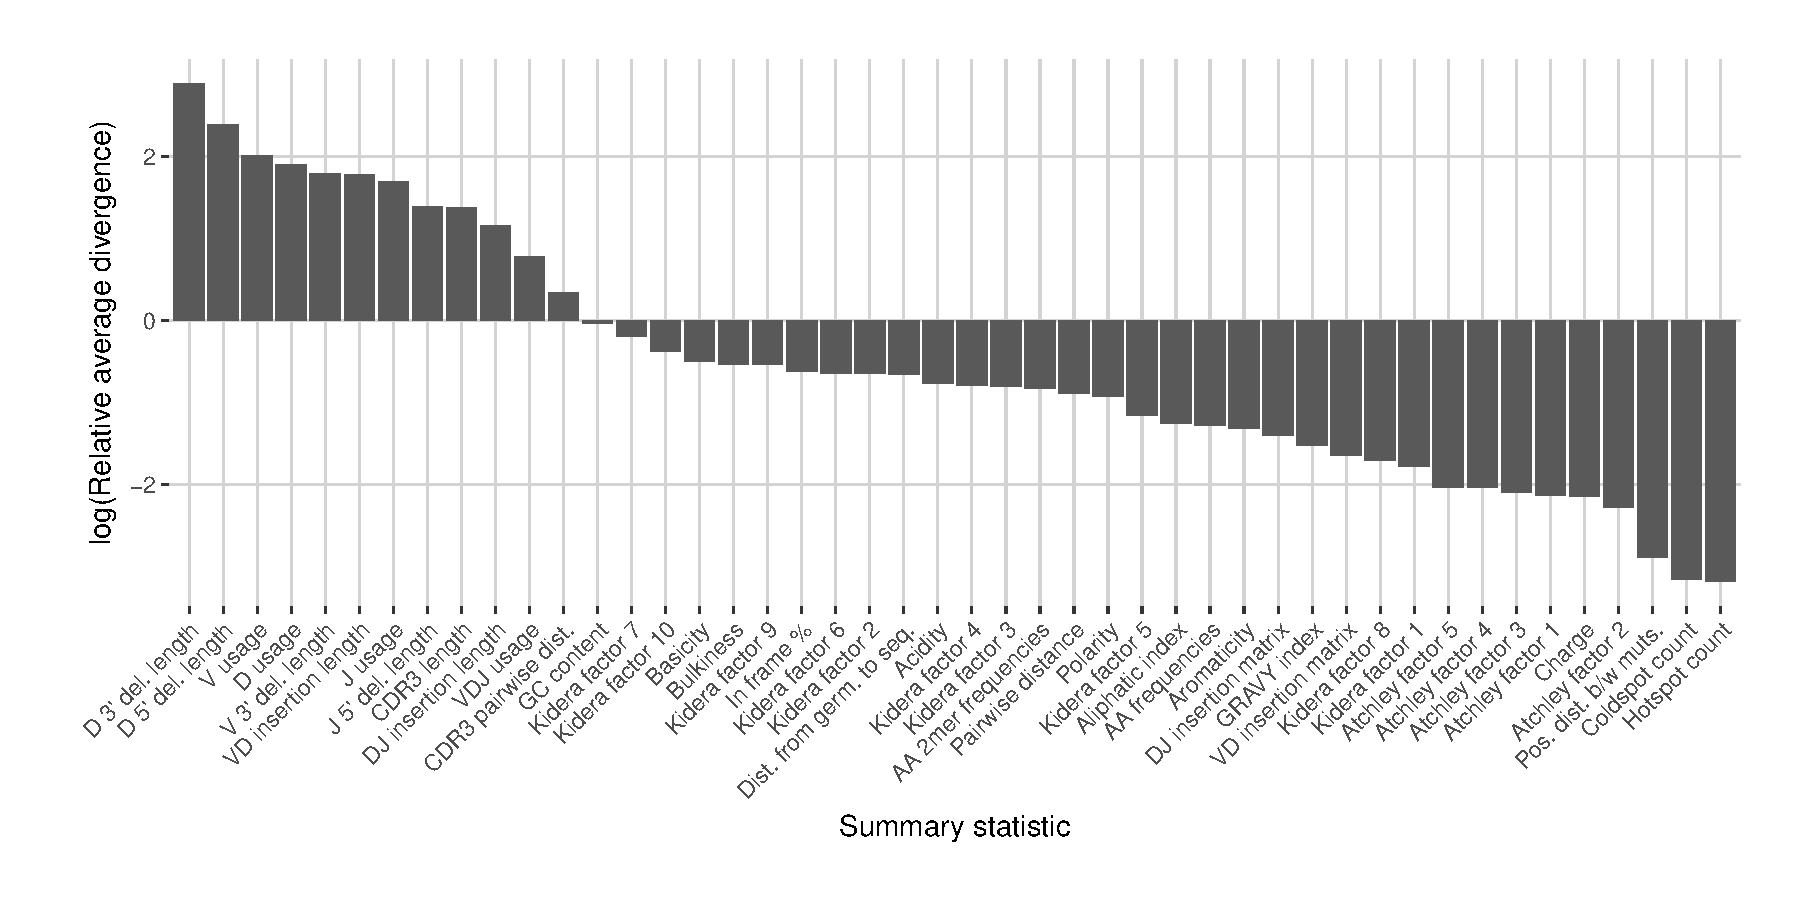
\includegraphics[width=\linewidth]{Figures/PartisScores/obs_score_plot.pdf}
    	\caption{$\text{score}_\text{obs}$ values for each statistic.}
    	\label{fig:ObsScoresBCR}
	\end{subfigure}
	\begin{subfigure}{\textwidth}
    	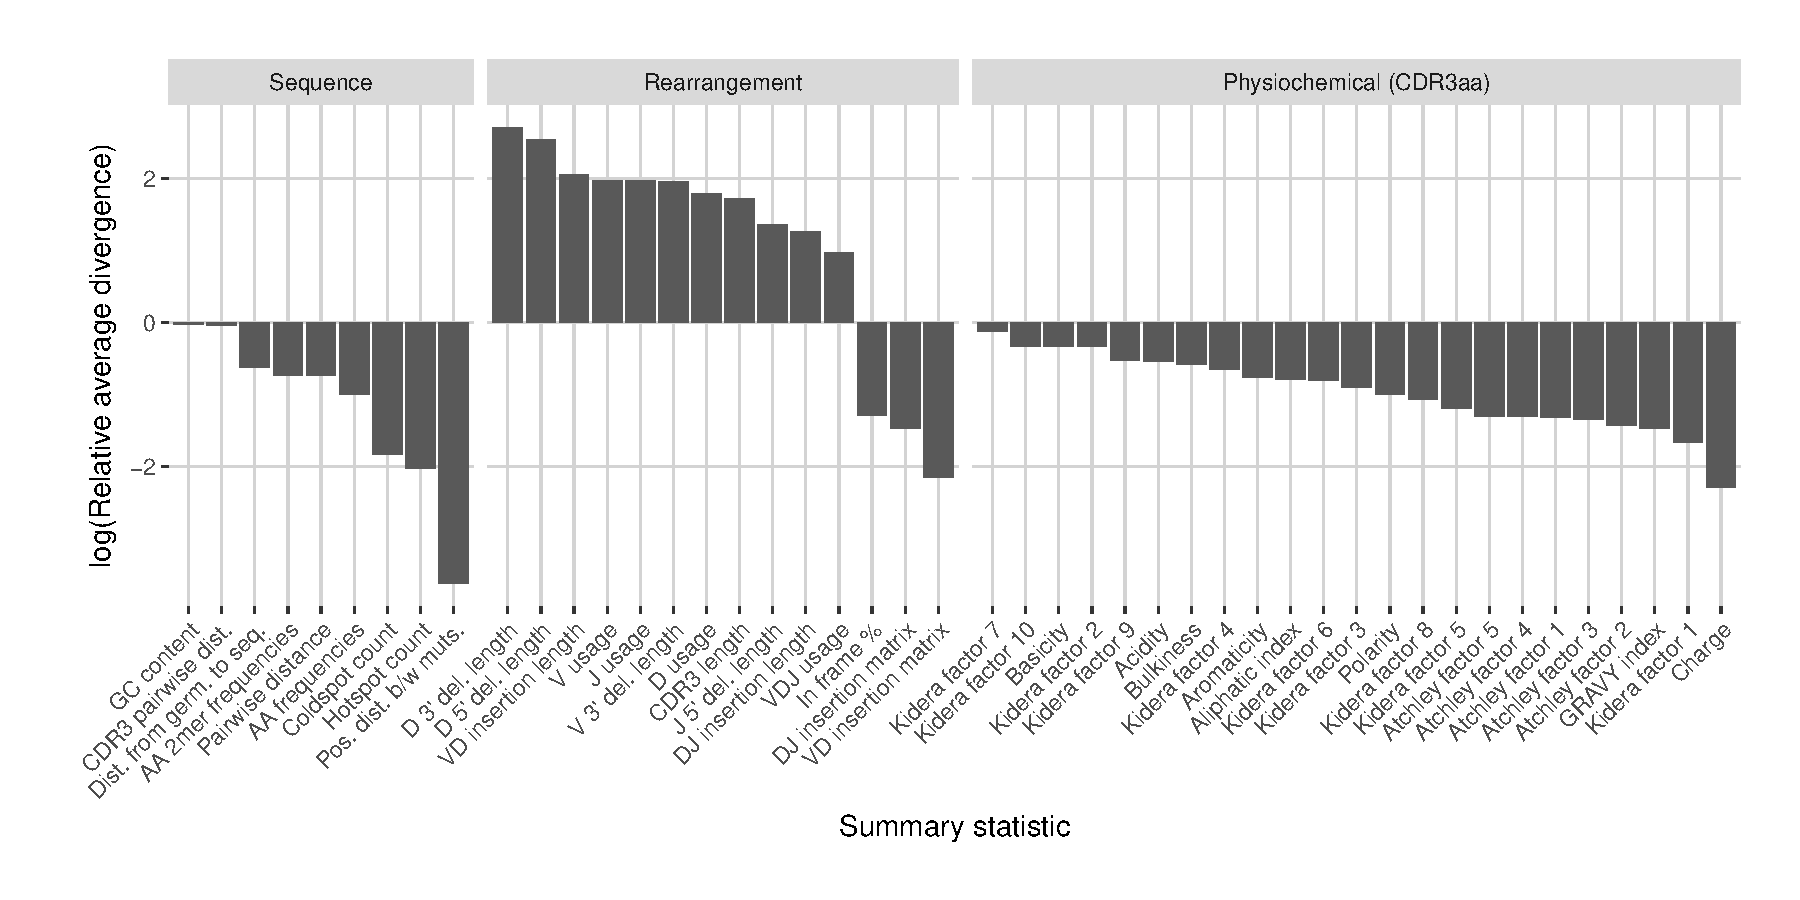
\includegraphics[width=\linewidth]{Figures/PartisScores/sim_score_plot.pdf}
    	\caption{$\text{score}_\text{sim}$ values for each statistic.}
    	\label{fig:SimScoresBCR}
	\end{subfigure}
	\caption{Summary scores, denoted as "log(Relative average divergence)" due to the form of Equations \ref{eq:ScoreObs} and \ref{eq:ScoreSim}, for each statistic in the \partis\ model validation experiment. For both cases, a high score indicates a well-replicated statistic by the simulations with respect to their corresponding experimental repertoires of functional IgH sequences.}
\end{figure}
Like \texttt{igor}, we see that \texttt{partis} simulations also excel at replicating gene usage and indel statistics, while also replicating CDR3 length distributions well.
However, \texttt{partis} struggles to recapitulate VD and DJ insertion matrices, which are not explicitly included in the model.
This contrasts \texttt{igor} which incorporates these insertion matrices during model fitting, and thus recapitulates these matrices well.
The other statistics yield scores ranging from slightly to very negative, with many mutation-related summaries like positional distance between mutations, and hot and cold spot counts, not being well-captured.
This is not very surprising as \texttt{partis} does not incorporate these quantities into the model fitting process, but does suggest that these sorts of quantities may need to be more explicitly accounted for in BCR generative models if more realistic simulations are desired.


Figure~\ref{fig:SimScoresBCR} displays the simulation-based summary scores for the same datasets and simulations.
The scores are highly similar to those seen in Figure~\ref{fig:ObsScoresBCR}, with some summaries like positional distance between mutations and VD/DJ insertion matrices seeing a moderate drop.


\section*{Methods}
\subsection*{Divergence}
We elect the Jenson-Shannon (JS) divergence for most of our comparison functions.
The Jenson-Shannon divergence of probability distributions $P$ and $Q$ with densities $p(\cdot)$ and $q(\cdot)$ is a symmetrized Kullbeck-Leiber divergence, defined as
\begin{equation}
\text{JSD}\left(P \ || \ Q\right) := \frac{\text{KLD}\left(P || M\right) + \text{KLD}\left(Q || M\right)}{2}
\end{equation}
where $M := (P + Q)/2$ and $\text{KLD}(P || M)$ is the usual KL-divergence,
\begin{equation}
\text{KLD}\left(P_1 \ || \ P_2\right) := \operatorname{E}_{\mathbf X \sim P_1}\left[ \log\left(\frac{p_1(\mathbf X)}{p_2(\mathbf X)}\right) \right].
\end{equation}
In the case where $P$ and $Q$ are both discrete distributions, this becomes
\begin{equation}
\text{KLD}\left(P_1 \ || \ P_2\right) = \sum_{i \in \text{supp}(P_1)} p_1(i) \log\left( \frac{p_1(i)}{p_2(i)} \right)
\end{equation}
where $\text{supp}(P)$ is the countable support of distribution $P$.
Because the discrete formulation is much nicer to worth with than the continuous one, we discretize continuous samples and treat them as discrete data.
By default, we use $B = \max\left(\left\lceil \sqrt{\min(m, n)} \right \rceil, 2\right)$ bins of equal length, where $m = |\text{supp}(P)|$ and $n = |\text{supp}(Q)|$, which is designed to scale with the complexity of $m$ and $n$ simultaneously.
We also discard bins which would lead to an infinite KL divergence for numerical stability.

Sometimes it makes more sense to use other distance metrics, such as the sum of absolute differences, or $\ell_1$ divergence, for count data of categorical variables:
\begin{equation}\label{eq:SAD}
    d_{\ell_1}(R_1, R_2; c, \mathcal S) = \sum_{s \in \mathcal S} \left| c(s; R_1) - c(s; R_2) \right|.
\end{equation}
In words, \eqref{eq:SAD} iterates over each element $s$ in some set $\mathcal S$, calculates the count $c$ of $s$ within repertoires $R_1$ and $R_2$ respectively, takes the absolute difference of counts, and appends this to a rolling sum.
This metric is well suited for comparing marginal or joint V/D/J-gene usage distributions.
For example, if $\mathcal V$, $\mathcal D$, and $\mathcal J$ represent the germline sets of V, D, and J genes, respectively,
defining define usage $u$ of gene triple $(v, d, j) \in \mathcal V \times \mathcal D \times \mathcal J$ for repertoire $R$ as
\begin{equation}
u(R; v, d, j) = \#\left\{s \in R: s_v = v, s_d = d, s_j = j\right\},
\end{equation}
where e.g. $s_v = $ the V gene of $s$, then an appropriate divergence for the joint VDJ gene usage for repertoires $R_1$ and $R_2$ is
\begin{equation}
d(R_1, R_2; u, \mathcal V, \mathcal D, \mathcal J) = \sum_{v \in \mathcal V} \sum_{d \in \mathcal D} \sum_{j \in \mathcal J} \left| u(v, d, j; R_1) - u(v, d, j; R_2) \right|.
\end{equation}
This divergence is also relevant for computing amino acid frequency and 2mer frequency distributions.
Note that we can normalize the counts to become relative frequencies and apply the $\ell_1$ metric on the resultant scale which may be better suited to the application, especially when dataset sizes differ notably.

\subsection*{Approximating distributions via subsampling and averaging}
Computing full summary distributions over large datasets can be intractable.
However, we can compute a Monte Carlo distribution estimate by repeatedly subsampling and aggregating summary values until convergence.
This idea is laid out in Algorithm~\ref{alg:DistributionAveraging}, which appends batch samples of $d$ to a rolling approximate distribution and terminates when successive distribution iterates have a JS divergence smaller than tolerance $\varepsilon$.
Note that continually appending values to a rolling vector is analogous to computing a rolling average, where the subject of the averaging is an empirical distribution rather than a scalar.
%BJO Should we make the algorithms figures?
\begin{algorithm}
    \caption{Compute automatic approximate distribution \\
        \textbf{Input:} repertoire $R$, summary $s$, batch size $m$, convergence tolerance $\varepsilon$\\
        \textbf{Output:} subsampled approximation to $d$}
    \label{alg:DistributionAveraging}
    \begin{algorithmic}
        \State $R_0 \gets \text{subsample}(R, m)$
        \State $d_0 \gets s(R_0)$
        \State $n \gets 1$
        \State error $\gets \infty$
        \While{error $> \varepsilon$}:
        \State $R_\text{samp} \gets \text{subsample}(R, m)$
        \State $d_\text{samp} \gets s(R_\text{samp})$
        \State $d_n \gets \text{concatenate}(d_{n-1}, d_\text{samp})$
        \State error $\gets \text{JSD}(d_{n-1}, d_n)$
        \State $n \gets n + 1$
        \EndWhile
    \end{algorithmic}
    \Return $d_n$
\end{algorithm}

An alternative would be to simply compute the distribution on one subsample of the data and use this as an approximate distribution.
The main advantage of Algorithm~\ref{alg:DistributionAveraging} over such an approach is that it provides a sense of how close the approximation is to the full distirbution via the tuning parameter $\varepsilon$, while automatically determining the size of the subsample.
The algorithm can also be tuned according to batch size $m$, which \texttt{sumrep} takes to be 30 by default.
We conduct a performance analysis of Algorithm~\ref{alg:DistributionAveraging} in Appendix A and empirically demonstrate efficiency gains in a variety of realistic settings without sacrificing much accuracy.

Some summaries induce distributions for which Algorithm~\ref{alg:DistributionAveraging} is ill-suited.
This occurs when a summary applied to a subset of a dataset does not follow the same distribution as the summary applied to the full dataset.
For example, consider the nearest neighbor distance of a sequence $s_i$ with respect to a multiset of sequences $R$ (i.e. elements in $R$ can have multiplicity $\ge 1$),
\begin{equation}
d_\text{NN}(s_i, R) := \min_{s \in R \setminus \{s_i\}} d(s_i, s),
\end{equation}
where $d(\cdot, \cdot)$ is a string metric (e.g. the Levenshtein distance).
If we take any subset $S$ of $R$, then $d_\text{NN}(s_i, S) \ge d_\text{NN}(s_i, R)$ $\forall i$, since $R$ will have the same sequences to iterate over, and possibly more sequences, which can only result in the same or a smaller minimum.


In this case, we can still obtain an unbiased approximate to the nearest neighbor distance distribution using the following modification of Algorithm~\ref{alg:DistributionAveraging}.
For each iteration, sample a small batch $B = (s_1, \dotsc, s_b)$ of $b$ sequences, and compute $d_\text{NN}$ of each $s_i$ to the full repertoire $R$.
Since each batch $B$ computes the exact nearest neighbor with respect to $R$, we get unbiased estimates of $d_\text{NN}$ for each $s \in B$.
Thus, appending batches to a running distribution until convergence as in Algorithm~\ref{alg:DistributionAveraging} will produce increasingly refined, unbiased approximations as the tolerance decreases.
Algorithm~\ref{alg:NNDistributionAveraging} explicates this procedure.

Algorithm~\ref{alg:NNDistributionAveraging} may yield a high runtime if $R$ is large, the sequences in $R$ are long, or the tolerance is small.
Nonetheless, we empirically demonstrate in Appendix B that in the case of typical BCR sequence reads, even very small tolerances incur reasonable runtimes, and when $R$ is large, the algorithm can be more than 100 times faster than computing the full distribution on $R$.

\begin{algorithm}
    \caption{Compute automatic approximate nearest neighbor distance distribution\\
        \textbf{Input:} repertoire $R$, distance $d$, batch size $m$, convergence tolerance $\varepsilon$\\
        \textbf{Output:} subsampled approximation to $d_\text{NN}$}
    \label{alg:NNDistributionAveraging}
    \begin{algorithmic}
        \State $d_0 \gets \Call{doBatchStep}{R, m}$
        \State $n \gets 1$
        \State error $\gets \infty$
        \While{error $> \varepsilon$}:
        	\State $d_\text{samp} \gets \Call{doBatchStep}{R, m}$
        	\State $d_n \gets \text{concatenate}(d_{n-1}, d_\text{samp})$
        	\State error $\gets \text{JSD}(d_{n-1}, d_n)$
        	\State $n \gets n + 1$
        \EndWhile
            \Return $d_n$
    \end{algorithmic}
    \begin{algorithmic}
    \Function{doBatchStep}{$R, m$}
    \For{$i = 1, \dots, m$}:
		\State $s_i \gets \text{subsample}(R, 1)$
        \State $d_i \gets d_\text{NN}(s_i; R)$
	\EndFor
	\Return $(d_1, \dotsc, d_m)$
	\EndFunction
    \end{algorithmic}
\end{algorithm}

\subsection*{Model validation of \texttt{IGoR}}
We use the \texttt{igor -infer} to fit custom, dataset-specific models for each experimental dataset.
Since we are interested in many CDR3-based statistics and IGoR does not currently include inferred CDR3 sequences with rearrangement scenarios, we use IgBlast extract CDR3s for each sequence.
For each sequence, we consider only the rearrangement scenario with the highest likelihood as determined by IGoR.
When a list of more than one potential genes is given for the gene call, we restrict to only the first gene.
Several fields are renamed to match the AIRR specification when the definitions align without ambiguity.

Although IGoR is typically applied to non-productive sequences in order to capture the pre-selection recombination process, for this example application we wished to understand IGoR's ability to fit the complete repertoire directly without the need for an additional selection model (e.g.\ \cite{Elhanati2014-mf}).

We applied IGoR in this way to six datasets of TRB sequences from \cite{Britanova2016-iw}, which studied T cell repertoires from donors ranging from newborn children to centenarians.

\subsection*{Model validation of \texttt{partis}}

We use \texttt{partis} to infer custom generative models for each experimental dataset.
We use the \texttt{partition} command to incorporate possible clonal family clustering among sequences during inference, and then collapse each observed and simulated dataset so that each clonal family is represented by one sequence.
Since \texttt{partis} returns a list of the top most likely scenarios for each rearrangement event, we consider only the scenario with the highest model likelihood for each sequence.
We denote the \texttt{indel\_reversed\_seqs} field as \texttt{sequence\_alignment} and \texttt{naive\_seq} as \texttt{germline\_alignment} as they adhere to these definitions from the AIRR schema.
Several other fields are renamed to match the AIRR specification when the definitions align without ambiguity.

Then, we compute the comparisons or divergences between each observed-simulated pair as well as between each of the observed datasets.
For each comparison, we subsample one receptor per clonal family to get a dataset consisting of ``unique clones'', for both the observed and simulated datasets.
We do this since \texttt{partis simulate} draws from distributions over clonal families for each rearrangement event as inferred from \texttt{partis partition}.
While it is possible to simulate multiple leaves for each rearrangement, it is not obvious how to best synchronize this with the observed clonal family distributions.
For example, if we had one clonal family with 1,000 members, and 99 singleton clonal families, we could try to coerce the simulator to produce on average a (roughly) size-1,000 clonal family for every 99 singletons.
However, it seems like this is highly contrived to the nature of our experimental sample, and does not clearly mimic the true repertoire dynamics of the individual from which the dataset was obtained.
Also, there is ambiguity to whether the rearrangement parameters for this size-1,000 clonal family should always match those of the observed size-1,000 clonal family, or if they should be sampled in some random fashion.
Hence, it seems more principled to subsample to unique clones and examine clonal family dynamics without dealing with abundance biases.


\subsection*{Scoring summary statistic replication by model}
%EM Would it be worth using some of these figures https://github.com/matsen/talks/tree/gh-pages/figures/sumrep ? (I just invited you.) I think that we're used to this framework but it may be a little strange for others.
%BJO Yes! Though I might have to put this off until after the WG meeting.
We wish to measure how well a given statistic is replicated when a model performs simulations using parameters inferred from an observed repertoire dataset.
One approach is to score the statistic $s$ based on the average divergence of observations to their simulated counterparts when applying $s(\cdot)$, and the average divergence of observations to other observations when applying $s(\cdot)$.
Suppose we have $k$ different experimental repertoires of immune receptor sequences, and let $R_{i, \text{obs}}$ and $R_{i, \text{sim}}$, $1 \le i \le k$, denote the $i$th observed and simulated repertoire, respectively.
For a given statistic $s$, let $\mathcal D_s(R_1, R_2)$ be the divergence of repertoires $R_1$ and $R_2$ with respect to $s$.
We can score a simulator's ability to recapitulate $s$ from the observed repertoire to the simulated via
\begin{equation}\label{eq:ScoreObs}
    \text{score}_\text{obs}(s) :=
    \log \left(
        \frac{
            \frac{1}{\frac{1}{2} k\left(k - 1\right)}
            \sum_{i=1}^{k}
            \sum_{j \ne i}
                \mathcal D_s\left(R_{i, \text{obs}}, R_{j, \text{obs}}\right)
        }
        {
            \frac{1}{k}
            \sum_{i = 1}^k
                \mathcal D_s \left( R_{i, \text{obs}}, R_{i, \text{sim}} \right)
        }
    \right).
\end{equation}
For a given summary $s$, score$_\text{obs}$ will be positive if the simulated repertoires tend to look more like their experimental counterparts in terms of this summary than experimental repertoires look like other experimental repertoires, and negative if experimental repertoires tend to look more like other experimental repertoires than they do their simulated counterparts.
In other words, this scores how well a simulator can differentiate $s$ from an experimental repertoire among other repertoires, and recapitulate $s$ into its simulation.
%BJO Does the below sentence make sense? For example, If the numerator is twice as high as the denominator, the score would be "2", and inverting the ratio would give "1/2". However, taking the log would yield 0.301 and -0.301, respectively. This makes the bar charts above easier to interpret.
Applying the log to the ratio allows for the magnitudes of scores to be directly comparable (so that a summary with score $a > 0$ does as well as a summary with score $-a < 0$ does poorly).

Another related score would be comparing the average divergence of observations to their simulated counterparts, and the average divergence of simulations to other simulations.
Formally, this is
\begin{equation}\label{eq:ScoreSim}
    \text{score}_\text{sim}(s) :=
    \log \left(
        \frac{
            \frac{1}{\frac{1}{2} k\left(k - 1\right)}
            \sum_{i=1}^{k}
            \sum_{j \ne i}
                \mathcal D_s\left(R_{i, \text{sim}}, R_{j, \text{sim}}\right)
        }
        {
            \frac{1}{k}
            \sum_{i = 1}^k
                \mathcal D_s \left( R_{i, \text{obs}}, R_{i, \text{sim}}\right)
        }
    \right).
\end{equation}
This value for a given summary will be negative if simulated repertoires tend to look more like their experimental counterparts (small $\mathcal D$ on the denominator) in terms of this summary than simulated repertoires look like other simulated repertoires, and positive if the simulated repertoires tend to look more alike.

We compute these scores for the analyses of \texttt{partis} and \texttt{igor} simulations in the Results section.
However, this framework can be used to validate any immune receptor repertoire simulator which outputs the fields compatible with the summaries in Table~\ref{tab:SummaryStatistics}, or more generally any set of summaries outside of the scope of \texttt{sumrep}, for any model-based simulator.

A feature of our methodology is that we use the same tool to produce simulations that we used to produce the annotations.
To examine the sensitivity of this method, we performed a separate analysis by obtaining dataset annotations from standalone IgBlast \cite{Ye2013-kl}, and comparing these to simulations based on \texttt{partis} annotations using IMGT germline databases.
We did not perform a similar analysis for \texttt{igor} annotations since IgBlast was used to infer CDR3s within the \texttt{igor} workflow.
This is discussed in detail in Appendix C.


\subsection*{Materials}
The raw data for the TCR summary divergence MDS analysis comes from \cite{Pogorelyy2018-ak}, which was postprocessed into a suitable format for analysis.

For the TCR model validation analysis, we use several datasets from \cite{Britanova2016-iw}.
For tractability purposes, we chose the six datasets with the fewest number of sequence reads; the number of reads from these six datasets used in the analysis ranged from 37,363 sequences to 243,903 sequences.
%BJO - Trying to run \texttt{igor} on larger datasets would often throw a segmentation fault. If this is a concern, we could choose a dataset from each of five individuals and subsample each dataset to, say, 50,000 sequences. But I don't think this would change the result that much.
These datasets consist of consensus RNA sequences assembled using UMIs.
Most of these sequences are functional; as previously described, for this example application we are benchmarking IGoR's ability to fit complete repertoires rather than only non-functional repertoires as described above.

The data for the BCR model validation analyses originated from samples and 454 data published in \cite{Laserson2014-dx}, with the MiSeq data and processed data published in \cite{Gupta2017-ve} used for our analyses.
These datasets represent repertoires of three human donors from two separate time points (1 hour and 8 days) following an influenza vaccination.
The number of reads from these six datasets used in the analysis range from 14,733 to 31,952 sequences.




\section*{Discussion}
We have presented a general framework for efficiently summarizing, comparing, and visualizing Rep-Seq datasets, and applied it to several questions of scientific interest.
One can imagine many further applications of \texttt{sumrep}, as well as promising avenues of research.

Similar tools: \cite{Nazarov2015-ok,Shugay2015-ur}.
TODO: Look for others.

A natural extension of the model validation in this report would be to assess the performance of many competing repertoire analysis tools over a larger group of datasets.
Moreover, it would likely be useful to perform separate analyses restricted to different CDRs and framework regions, as physiochemical characteristics of these regions can differ greatly.


Contrasting repertoires in the context of antigen response or vaccination design and evaluation may shed some light on which summaries can distinguish between such covariates.
\texttt{sumrep} could also be used to evaluate the extent to which artificial lymphocyte repertoires look like natural ones~\cite{Finlay2012}.

\section*{Acknowledgements}
We thank Misha Pogorelyy for kindly providing post-processed data from \cite{Pogorelyy2018-ak}.


\bibliographystyle{plain}
\bibliography{main}

\beginsupplement

\section*{Appendix A: Performance of distribution subsampling algorithms}
Here, we run Algorithm~\ref{alg:DistributionAveraging} on \texttt{p\_f1} subsampled without replacement to 10,000 sequences for tractability.
We compute the pairwise distance distribution of CDR3 sequences for the full subsampled dataset, and approximate distributions with tolerances $\varepsilon \in \left\{0.1, 0.001, \dotsc, 10^{-7} \right\}$.
We replicate this experiment for 10 trials so that the subsampled dataset remains the same, but a new instance of the subsampling algorithm is run each time.
\begin{figure}
    \begin{subfigure}{.5\textwidth}
        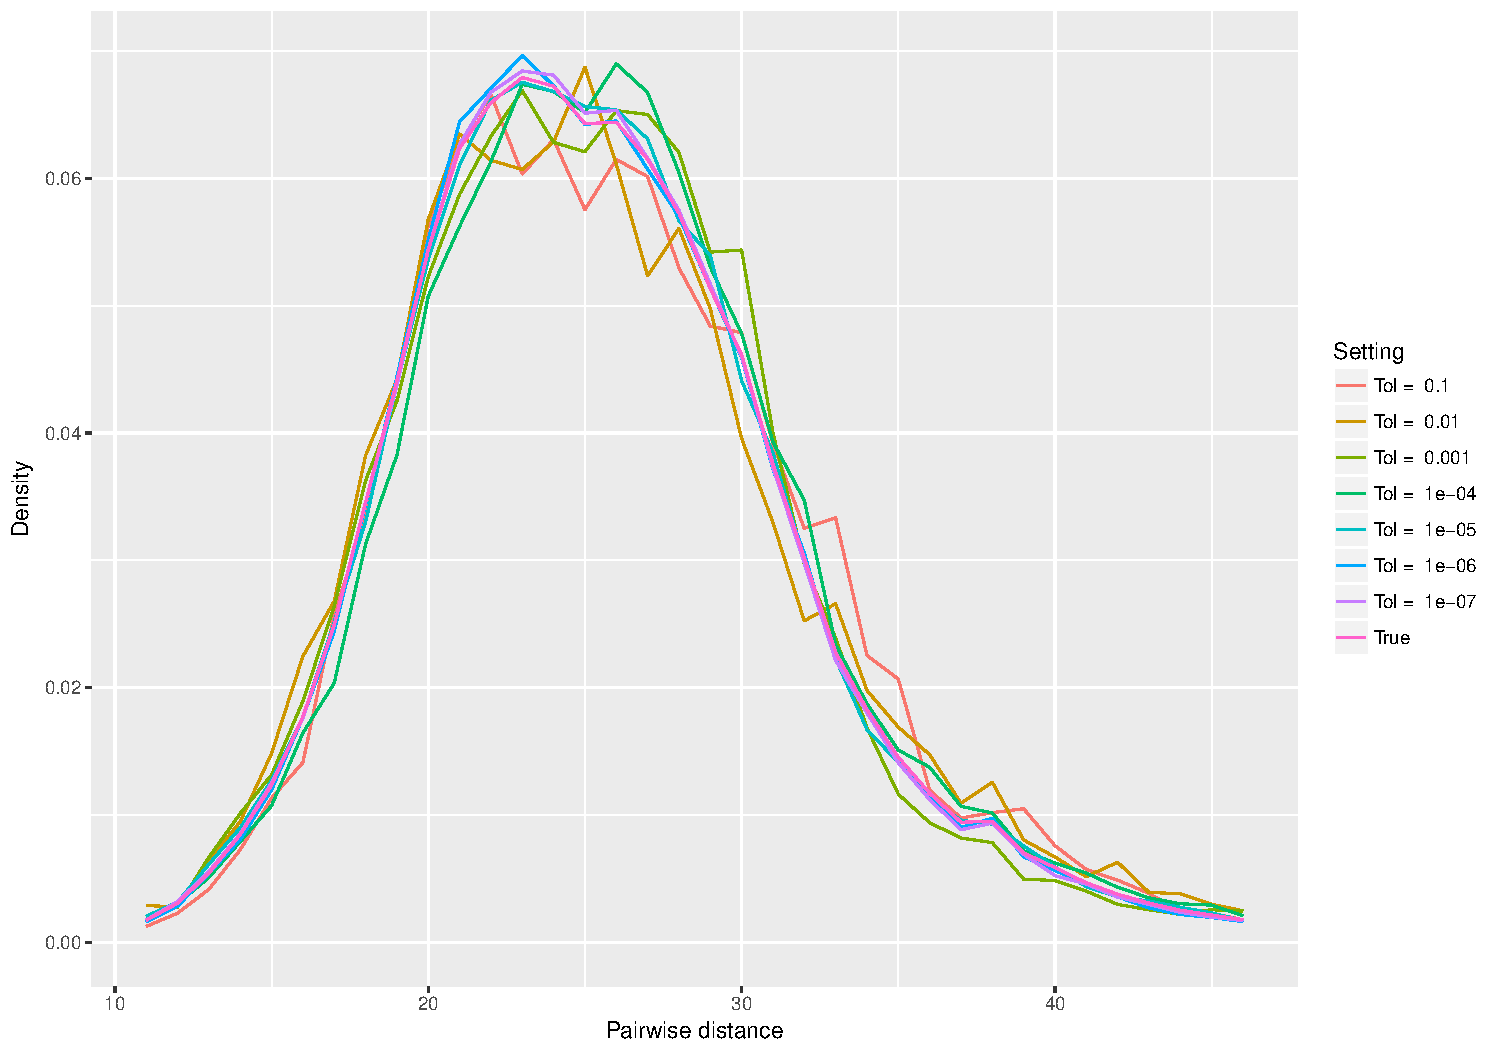
\includegraphics[width=\linewidth]{Figures/PairwiseDistance/freqpoly_by_tol.pdf}
   		\caption{Frequency polygons of true and subsampled pairwise distance distributions by tolerance.}
    	\label{fig:FreqPoly}
    \end{subfigure}
    \begin{subfigure}{.5\textwidth}
        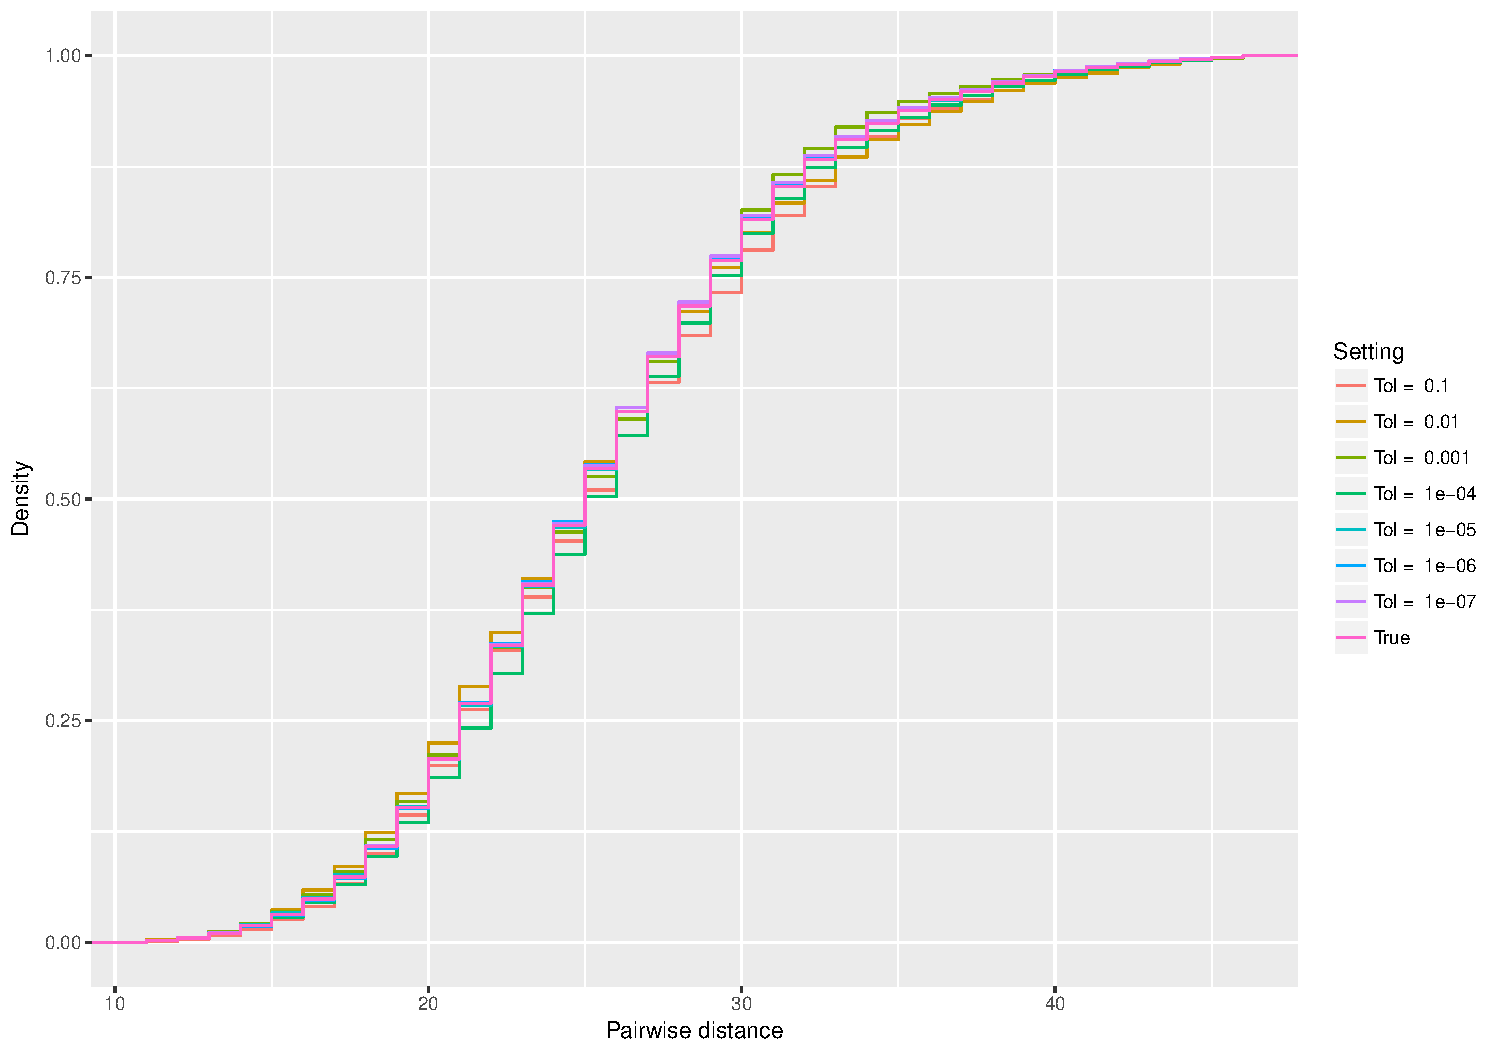
\includegraphics[width=\linewidth]{Figures/PairwiseDistance/ecdf_by_tol.pdf}
    	\caption{Empirical c.d.f. of true and subsampled pairwise distance distributions by tolerance.}
    	\label{fig:ECDF}
    \end{subfigure}
    \begin{subfigure}{.5\textwidth}
        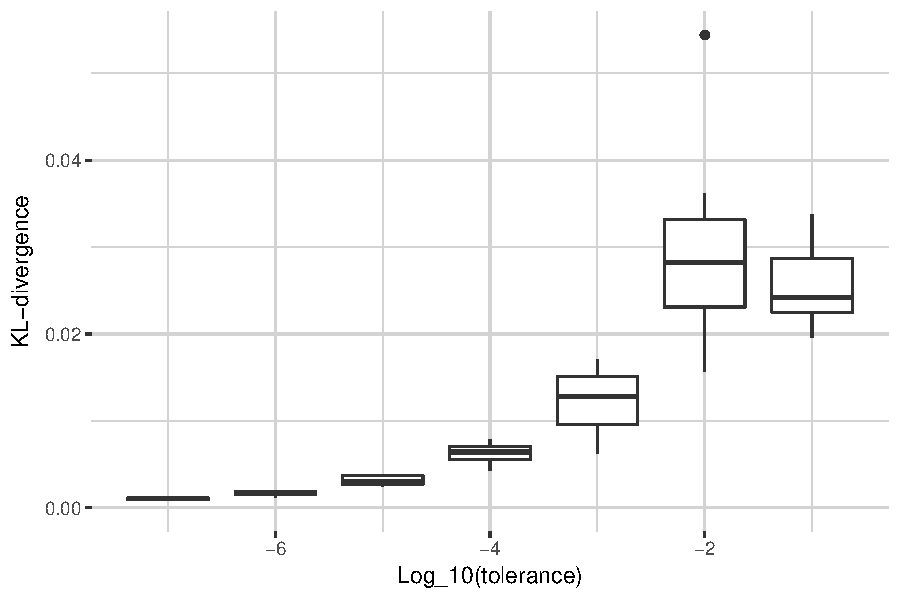
\includegraphics[width=\linewidth]{Figures/PairwiseDistance/div_by_tol.pdf}
    	\caption{KL-divergence to true pairwise distance distribution by tolerance, taken over 10 trials of the algorithm.}
    	\label{fig:Divergences}
	\end{subfigure}
    \begin{subfigure}{.5\textwidth}
    	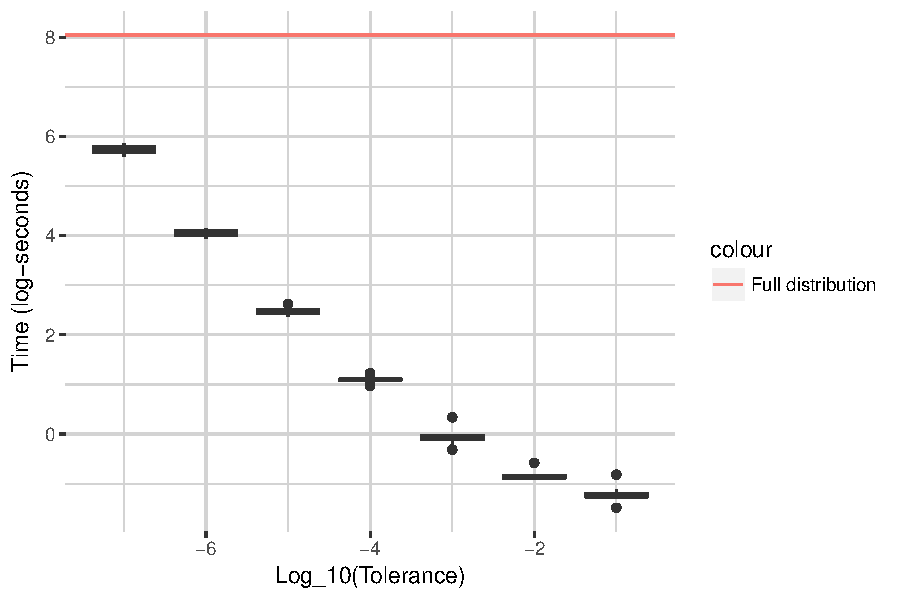
\includegraphics[width=0.9\linewidth]{Figures/PairwiseDistance/log_time_by_tol.pdf}
    	\caption{Runtime (in log-seconds) for Algorithm~\ref{alg:DistributionAveraging} by tolerance, taken over 10 trials.}
    	\label{fig:Times}
    \end{subfigure}
    %EM if we want these to get a "Figure XX" label the overall figure needs a caption.
    %BJO I don't believe I needed/wanted these sorts of labels for references, but I'm not against it either.
    %EM It looks quite strange to me to have (a), etc, but no figure number. Sorry!
    \caption{Performance of Algorithm~\ref{alg:DistributionAveraging} by tolerance applied to the pairwise distance distribution.}
\end{figure}
Figure~\ref{fig:FreqPoly} shows a frequency polygon of each distribution and figure~\ref{fig:ECDF} shows their empirical cumulative distribution functions.
We see that the approximate distributions appear to converge to the full distribution as the tolerance gets smaller.
Figure~\ref{fig:Divergences} displays the KL-divergence to the true distribution for each tolerance, again indicating convergence to the truth.
Figure~\ref{fig:Times} displays the runtimes and log-runtimes for each tolerance as well as the true "population" runtime for the full dataset; while the runtime grows exponentially as $\varepsilon \to 0$, the approximation algorithm is still much faster than computing the full distribution for each considered value of $\varepsilon$.

Next we investigate the effect of dataset size on the performance of Algorithm~\ref{alg:DistributionAveraging}.
For sample sizes $n \in \{\exp(5), \dotsc, \exp(9)\}$, we subsample \texttt{p\_f1} without replacement to $n$ sequences and compute the pairwise distance distribution of CDR3 sequences for the full subsampled dataset as well as those given by tolerances $\varepsilon \in \{0.1, 0.01, ..., 10^{-5} \}$.
We perform this experiment 10 times for each $n$.
Boxplots of the KL-divergence by $\log(n)$ and tolerance over all trials are displayed in Figure~\ref{fig:PDDivBySize}.
We see no obvious trend in the effect of dataset size on the KL-divergence for any choice of tolerance for the pairwise distribution.
Boxplots of the runtime (in log-seconds) by log(size) and tolerance are shown in Figure~\ref{fig:PDTimeBySize}, showing that runtime increases with sample size for high tolerance, but tends towards a constant runtime by sample size as tolerance decreases.
Boxplots of the log-efficiency by log(size) and tolerance are shown in Figure~\ref{fig:PDEfficiencyBySize}, where
\begin{equation}\label{eq:Efficiency}
	\text{Efficiency} :=
		\frac{\text{time to compute full distribution}
		}{
			  \text{time to compute approximate distribution}
		}.
\end{equation}
Here we plot efficiency on a log scale, so that the line $y=0$ corresponds to instances when the true and approximate routines have identical runtimes.
Thus, the region $y > 0$ corresponds to instances when Algorithm~\ref{alg:DistributionAveraging} outperforms the computation of the full nearest neighbor distribution.
For moderate to large datasets and reasonable choices of $\varepsilon$, the approximate routine is much more efficient than computing the full distribution.
Efficiency also appears to increase exponentially with dataset size, although decreases at least exponentially as tolerance decreases.
Nonetheless, the accuracy of Algorithm~\ref{alg:DistributionAveraging} applied to the pairwise distance distribution is scalable to large datasets while leading to large gains in runtime efficiency for reasonable choices of $\varepsilon$.

\begin{figure}
    \begin{subfigure}{0.5\textwidth}
        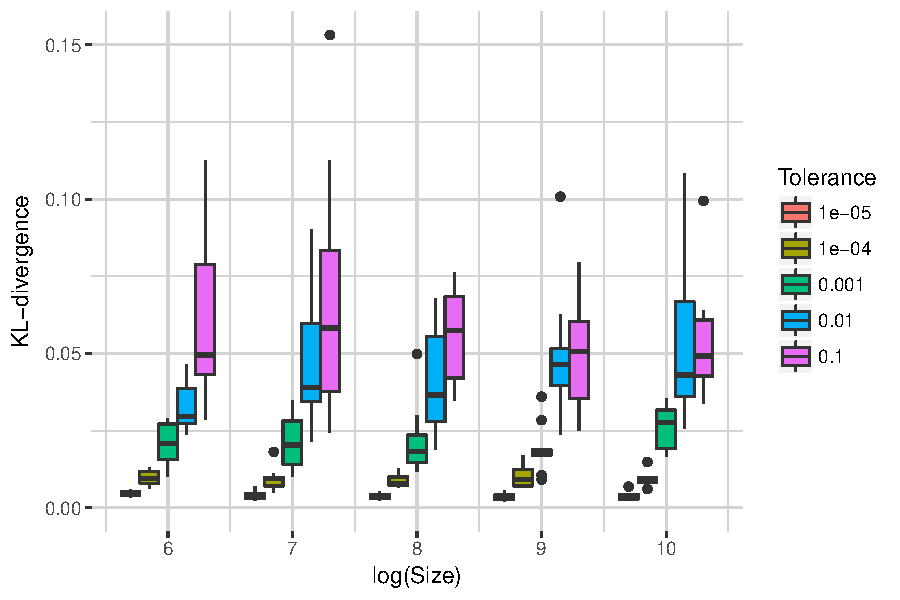
\includegraphics[width=\linewidth]{Figures/PairwiseDistance/div_by_size_and_tol.pdf}
        \caption{KL-divergence to true pairwise distance distribution by tolerance and log(size) of dataset, taken over 10 trials of the algorithm.}
        \label{fig:PDDivBySize}
    \end{subfigure}
    \begin{subfigure}{0.5\textwidth}
        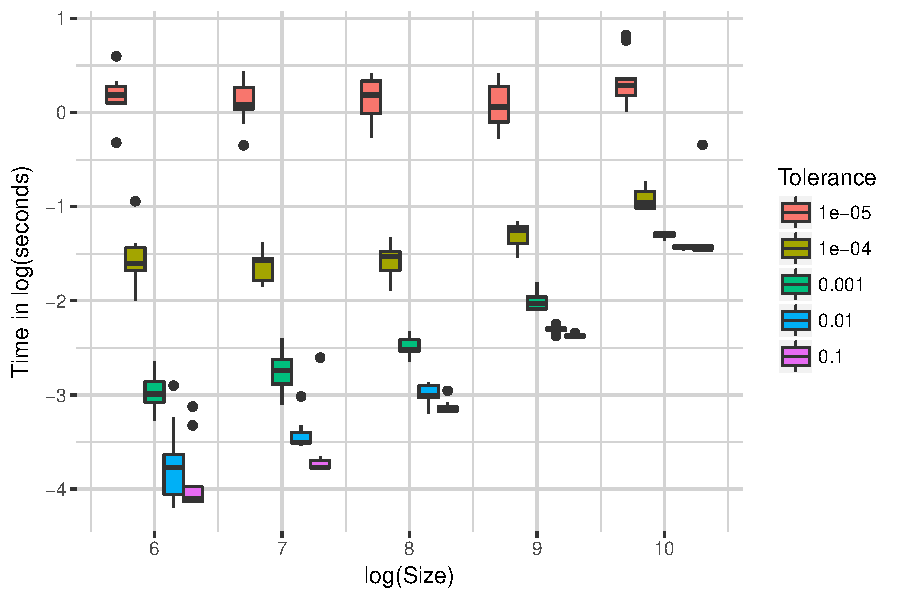
\includegraphics[width=\linewidth]{Figures/PairwiseDistance/time_by_size_and_tol.pdf}
        \caption{Runtime by tolerance and log(size) of dataset, taken over 10 trials of the algorithm.}
        \label{fig:PDTimeBySize}
    \end{subfigure}
    \begin{subfigure}{0.5\textwidth}
        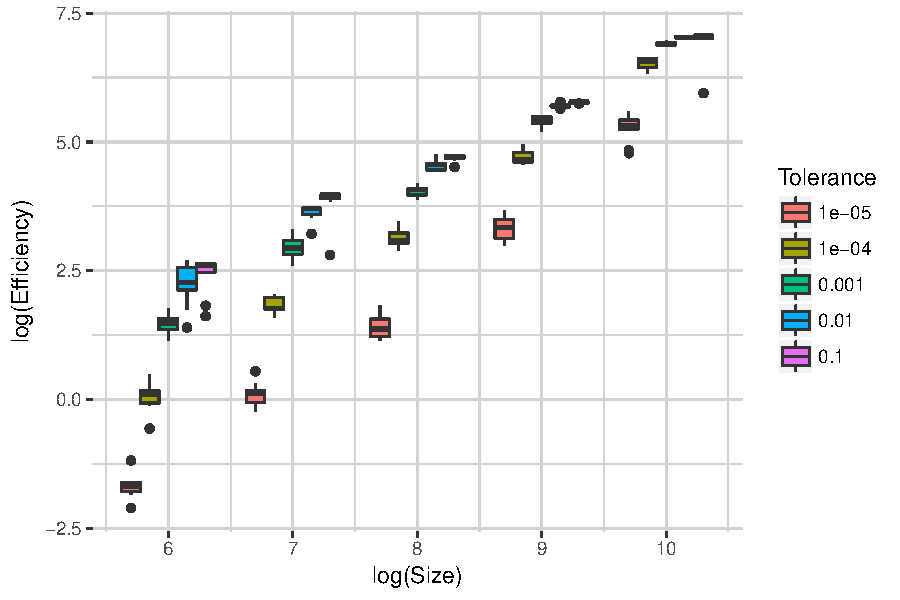
\includegraphics[width=\linewidth]{Figures/PairwiseDistance/efficiency_by_size_and_tol.pdf}
        \caption{Efficiency by tolerance and log(size) of dataset, taken over 10 trials of the algorithm.}
        \label{fig:PDEfficiencyBySize}
    \end{subfigure}
    \caption{Performance of Algorithm~\ref{alg:DistributionAveraging} by sample size and tolerance applied to the pairwise distance distribution.}
\end{figure}

%BJO - Rerunning this as I think the plot is outdated (1,000 seqs instead of 10,000)
Finally, we investigate the effect of summary statistic on the performance of Algorithm~\ref{alg:DistributionAveraging}.
We run the algorithm for the pairwise distance, GC content, hotspot count, coldspot count, and distance from germline to sequence distributions on \texttt{p\_f1} subsampled without replacement to 10,000 rows.
For each summary, we run the algorithm for tolerances $\varepsilon \in \{0.1, \dotsc, 10^{-5}\}$.
We perform this experiment 10 times for each (summary, $\varepsilon$) combination.
Figures~\ref{fig:DivBySummary}, \ref{fig:TimeBySummary}, and \ref{fig:EfficiencyBySummary} show the KL-divergence to the full dataset distributions, runtimes, and efficiencies, respectively, by summary and tolerance over all trials.
\begin{figure}
    \begin{subfigure}{0.5\textwidth}
        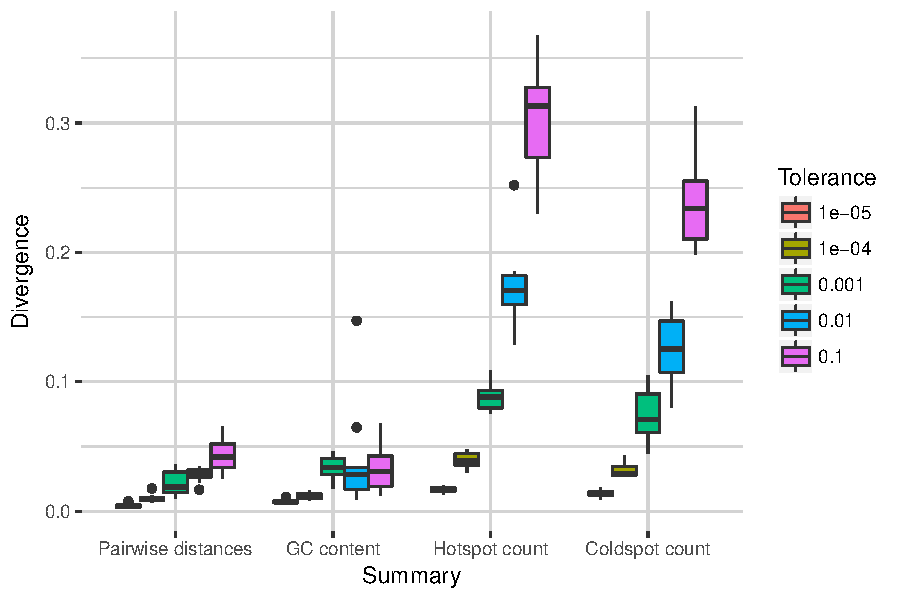
\includegraphics[width=\linewidth]{Figures/Multiple/div_by_summary_and_tol.pdf}
        \caption{KL-divergence to true summary distributions by tolerance, taken over 10 trials of the algorithm}
        \label{fig:DivBySummary}
    \end{subfigure}
    \begin{subfigure}{0.5\textwidth}
        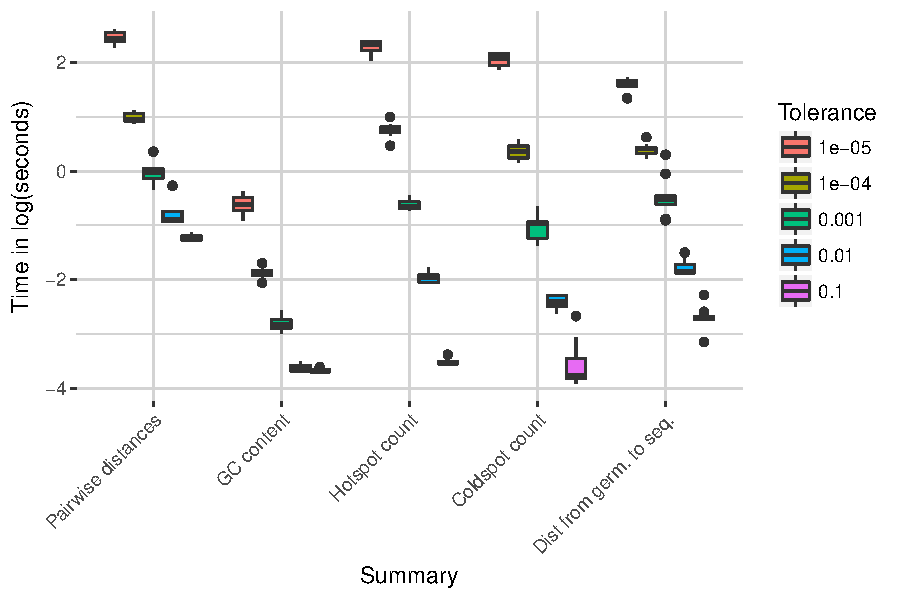
\includegraphics[width=\linewidth]{Figures/Multiple/time_by_summary_and_tol.pdf}
        \caption{Runtime by summary distribution and tolerance, taken over 10 trials of the algorithm}
        \label{fig:TimeBySummary}
    \end{subfigure}
    \begin{subfigure}{0.5\textwidth}
        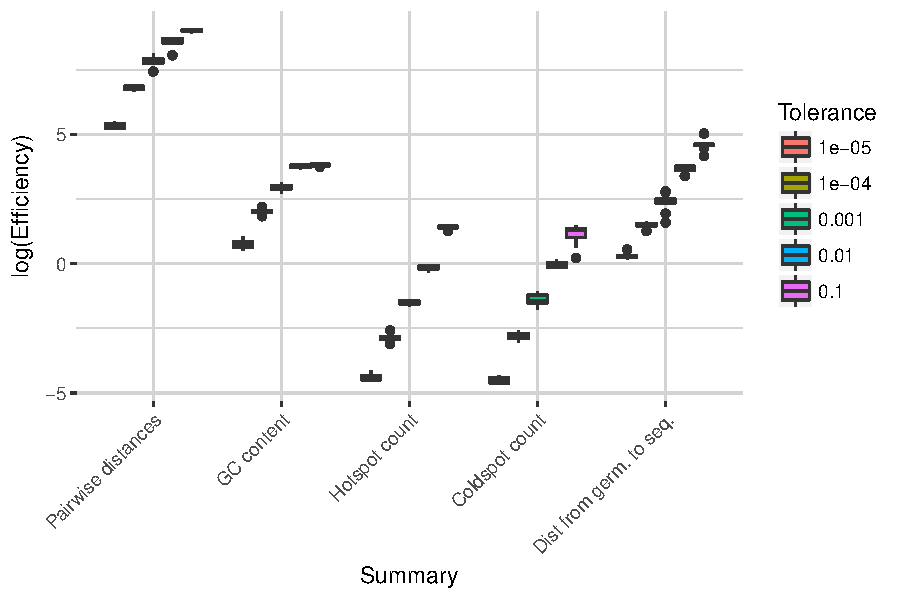
\includegraphics[width=\linewidth]{Figures/Multiple/efficiency_by_summary_and_tol.pdf}
        \caption{Efficiency by summary distribution and tolerance, taken over 10 trials of the algorithm}
        \label{fig:EfficiencyBySummary}
    \end{subfigure}
    \caption{Performance of Algorithm~\ref{alg:DistributionAveraging} by summary statistic and tolerance applied to the pairwise distance distribution.}
\end{figure}
We see that the KL divergence, runtime, and efficiency of the approximation routine depends on the summary in question.
In particular, the approximation routine for hotspot and coldspot count distributions does not yield as high of an efficiency for moderately low tolerance, and struggles to minimize the KL-divergence to the true distribution for higher tolerances.
This is likely due to the fact that the full hotspot and coldspot count distributions is extremely fast to compute even for large datasets.

These results suggest that convergence and efficiency will vary by summary, and the user should be aware of this fact when choosing whether to run the approximation routine as well as an appropriate tolerance.

\subsection*{Appendix B: Performance of nearest neighbor distribution subsampling algorithm}
Here, we assess the modification of the distribution approximation routine for the nearest neighbor distribution.
We run Algorithm~\ref{alg:NNDistributionAveraging} on \texttt{p\_f1} subsampled without replacement to 10,000 sequences for tractability.
We compute the nearest neighbor distribution of CDR3 nt sequences for the full subsampled dataset, and approximate distributions with tolerances $\varepsilon \in \left\{0.1, 0.001, \dotsc, 10^{-7} \right\}$.
We replicate this experiment for 10 trials in the same manner as detailed in Appendix A.

Figure~\ref{fig:NNFreqPoly} shows a frequency polygon of each distribution, and Figure~\ref{fig:NNECDF} shows their empirical cumulative distribution functions.
Figure~\ref{fig:NNDivergences} shows KL divergences of approximate distributions to the true distribution which decay as $\varepsilon \to 0$.
\begin{figure}
    \begin{subfigure}{.49\textwidth}
        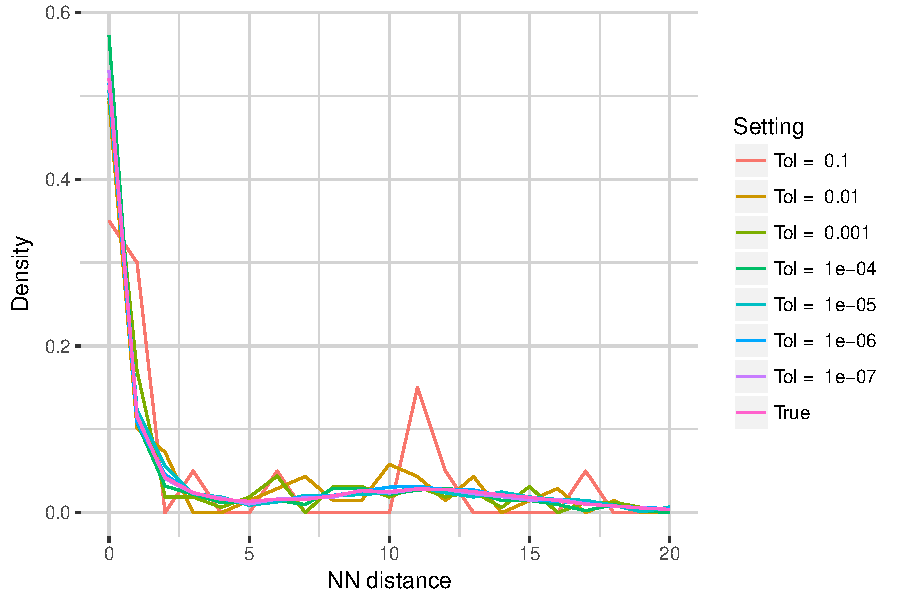
\includegraphics[width=\linewidth]{Figures/NearestNeighbor/CDR3/freqpoly_by_tol.pdf}
   		\caption{Frequency polygons of true and subsampled nearest neighbor distance distributions by tolerance.}
    	\label{fig:NNFreqPoly}
    \end{subfigure}
    \begin{subfigure}{.49\textwidth}
        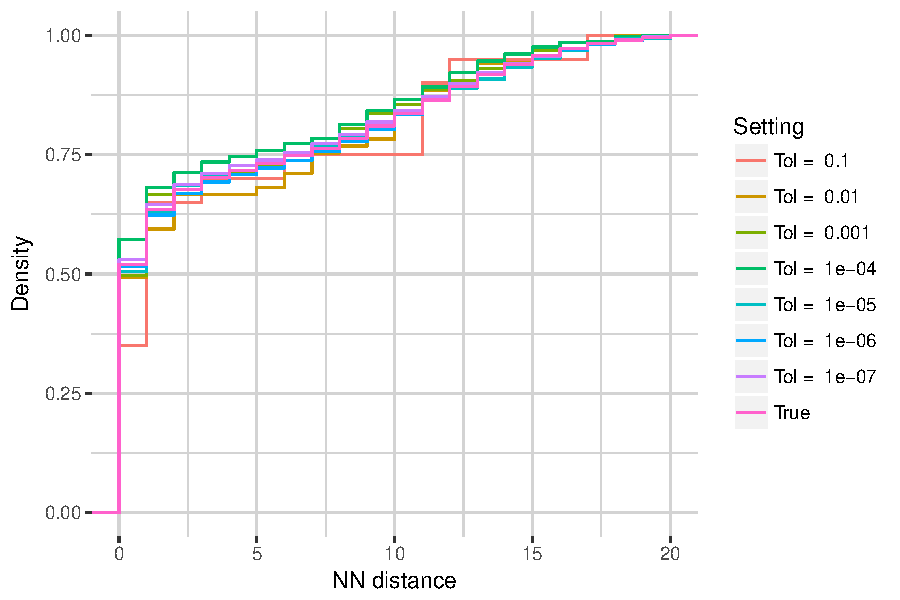
\includegraphics[width=\linewidth]{Figures/NearestNeighbor/CDR3/ecdf_by_tol.pdf}
    	\caption{Empirical c.d.f. of true and subsampled nearest neighbor distance distributions by tolerance.}
    	\label{fig:NNECDF}
    \end{subfigure}
    \begin{subfigure}{.49\textwidth}
        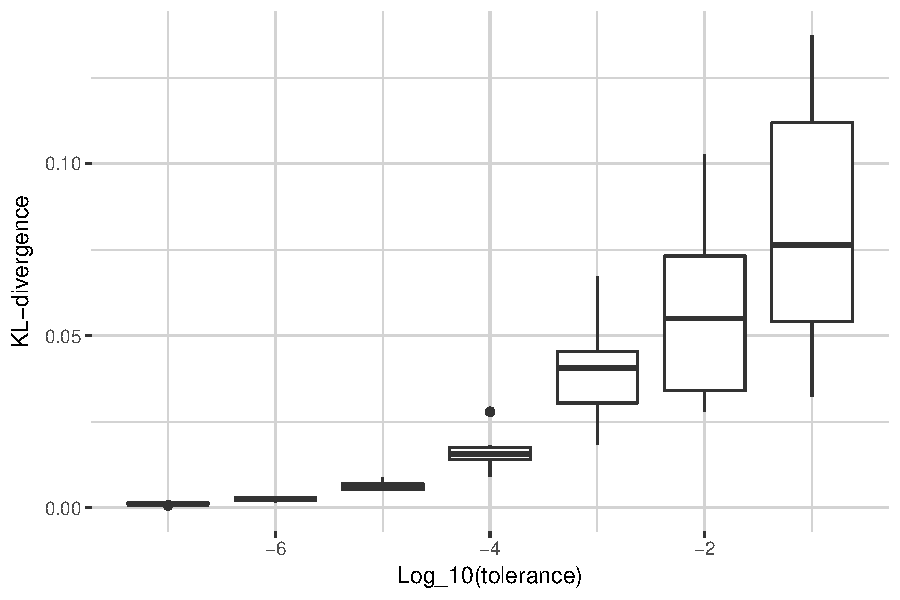
\includegraphics[width=\linewidth]{Figures/NearestNeighbor/CDR3/div_by_tol.pdf}
    	\caption{KL-divergence to true nearest neighbor distance distribution by tolerance, taken over 10 trials of the algorithm.}
    	\label{fig:NNDivergences}
	\end{subfigure}
	%BJO The captions aren't horizontally aligned -- way to fix?
    \begin{subfigure}{.49\textwidth}
    	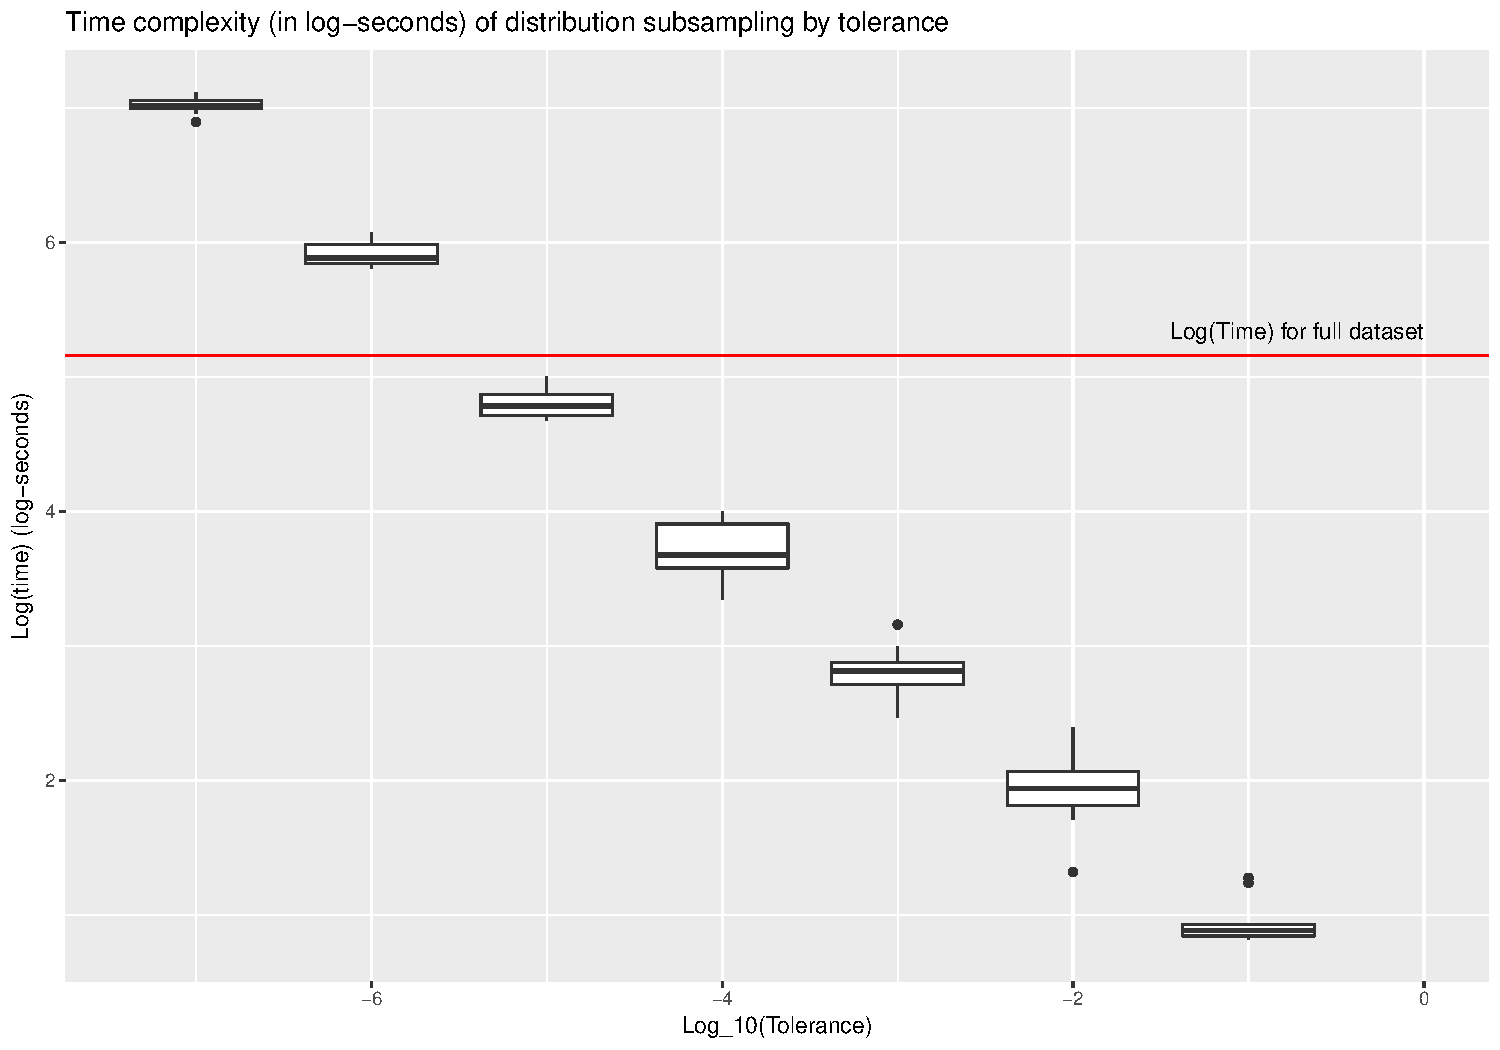
\includegraphics[width=0.9\linewidth]{Figures/NearestNeighbor/CDR3/log_time_by_tol.pdf}
    	\caption{Runtime (in seconds) and log-runtime (in log-seconds) for Algorithm~\ref{alg:NNDistributionAveraging} by tolerance, taken over 10 trials.}
    	\label{fig:NNTimes}
    \end{subfigure}
    \caption{Performance of Algorithm~\ref{alg:NNDistributionAveraging} by tolerance applied to the nearest neighbor distribution of CDR3nt sequences.}
\end{figure}
Indeed, these three figures indicate that the approximate distributions converge to the full distribution as $\varepsilon \to 0$.
Figure~\ref{fig:NNTimes} displays boxplots of the runtime in log-seconds for Algorithm~\ref{alg:NNDistributionAveraging} as well as the runtime to compute the full distribution.
In this case, we see that the Algorithm~\ref{alg:NNDistributionAveraging} becomes slower than computing the full distribution when $\varepsilon \lesssim 10^{-5}$.

To assess the effect of sequence lengths on Algorithm~\ref{alg:NNDistributionAveraging}, we perform the same experiment as above on pairwise aligned VDJ sequences (via the \texttt{sequence\_alignment} column rather than inferred CDR3 sequences.
These length distributions are different by about an order of magnitude.
We note that the pairwise aligned VDJ sequences are the default for Algorithm~\ref{alg:NNDistributionAveraging} within \texttt{sumrep}, although we anticipate users to examine this distribution for CDR3s as well as full V(D)J sequences.
We run Algorithm~\ref{alg:NNDistributionAveraging} on the same subsampled 10,000 sequences of \texttt{p\_f1}.

Figure~\ref{fig:NNFreqPolySequence} shows a frequency polygon of the same distributions, and Figure~\ref{fig:NNECDFSequence} shows their empirical cumulative distribution functions.
Moreover, Figures~\ref{fig:NNDivergencesSequence} and \ref{fig:NNTimesSequence} show the KL-divergences to truth and runtimes, respectively.
\begin{figure}
    \begin{subfigure}{.49\textwidth}
        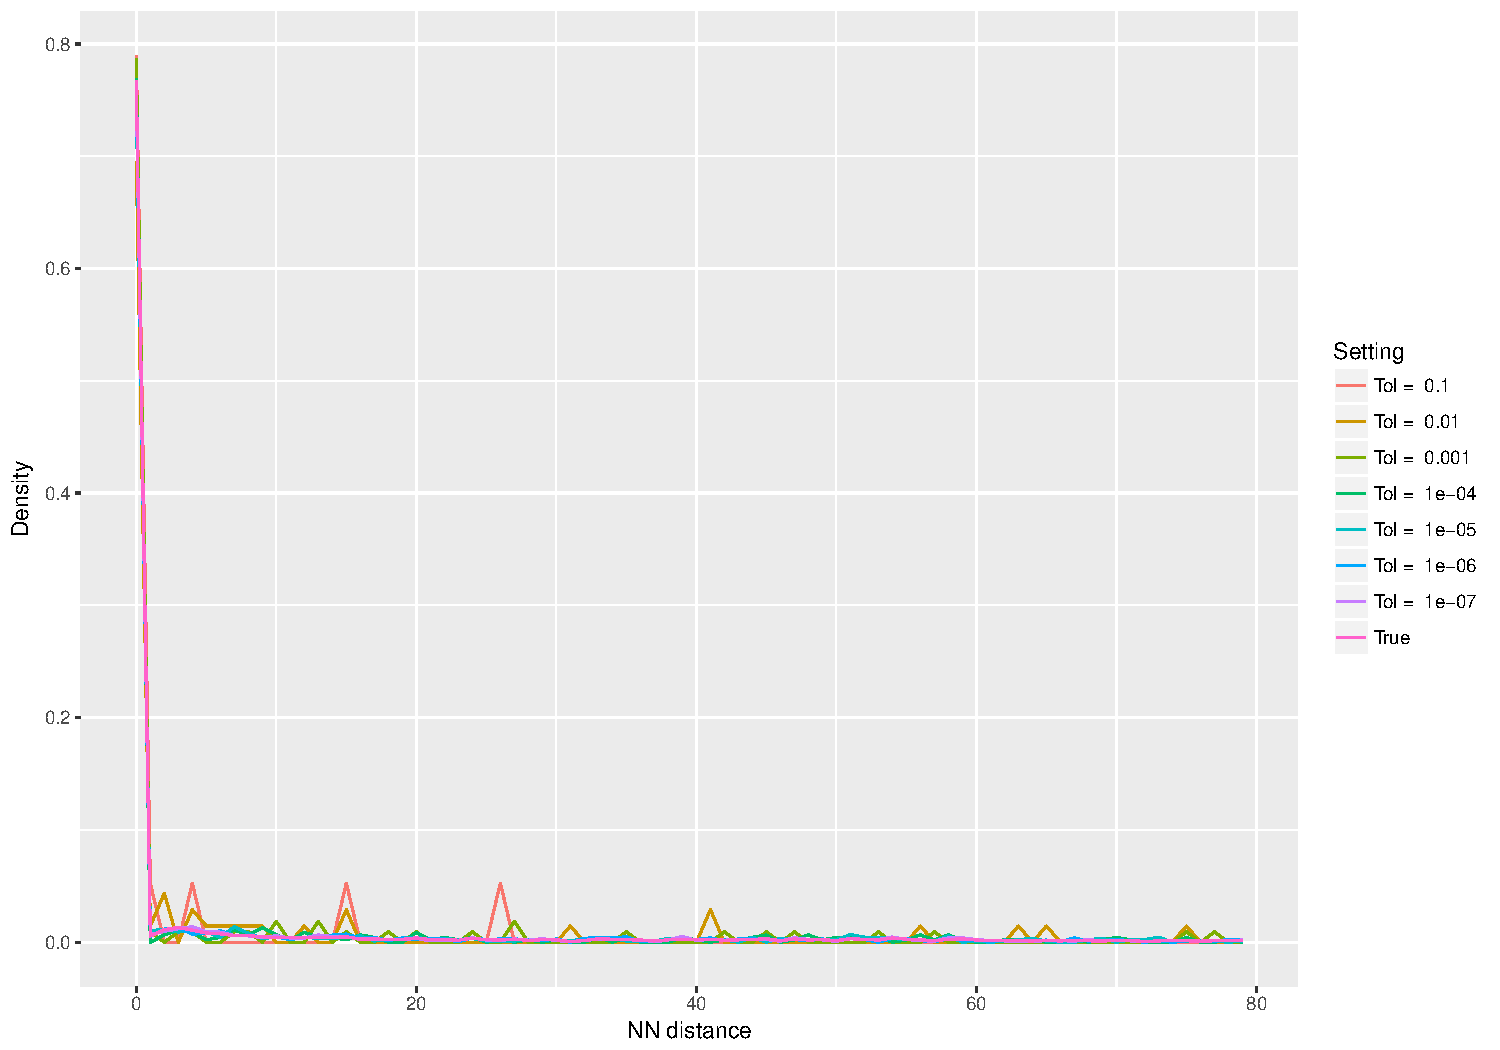
\includegraphics[width=\linewidth]{Figures/NearestNeighbor/Sequence/freqpoly_by_tol.pdf}
   		\caption{Frequency polygons of true and subsampled nearest neighbor distance distributions by tolerance.}
    	\label{fig:NNFreqPolySequence}
    \end{subfigure}
    \begin{subfigure}{.49\textwidth}
        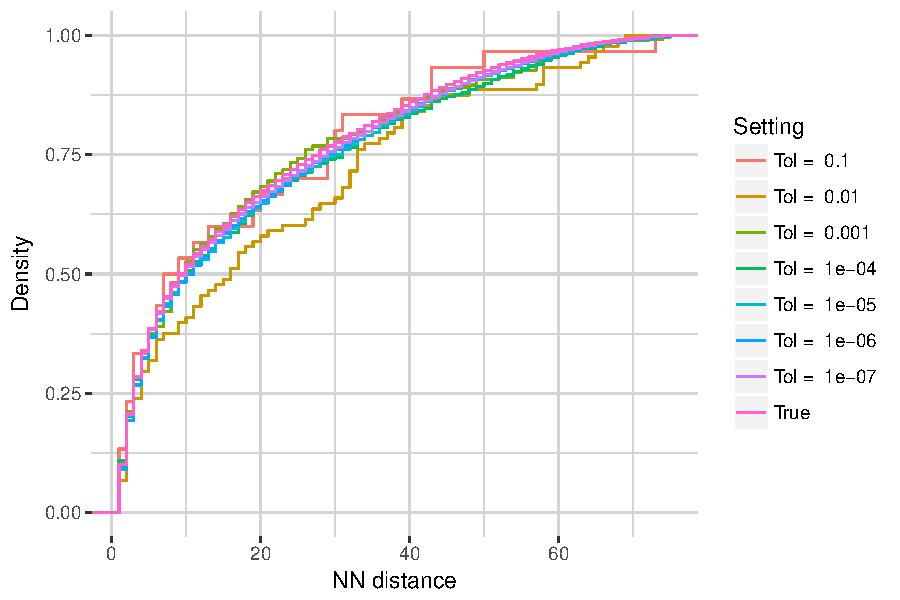
\includegraphics[width=\linewidth]{Figures/NearestNeighbor/Sequence/ecdf_by_tol.pdf}
    	\caption{Empirical c.d.f. of true and subsampled nearest neighbor distance distributions by tolerance.}
    	\label{fig:NNECDFSequence}
    \end{subfigure}
    \begin{subfigure}{.49\textwidth}
        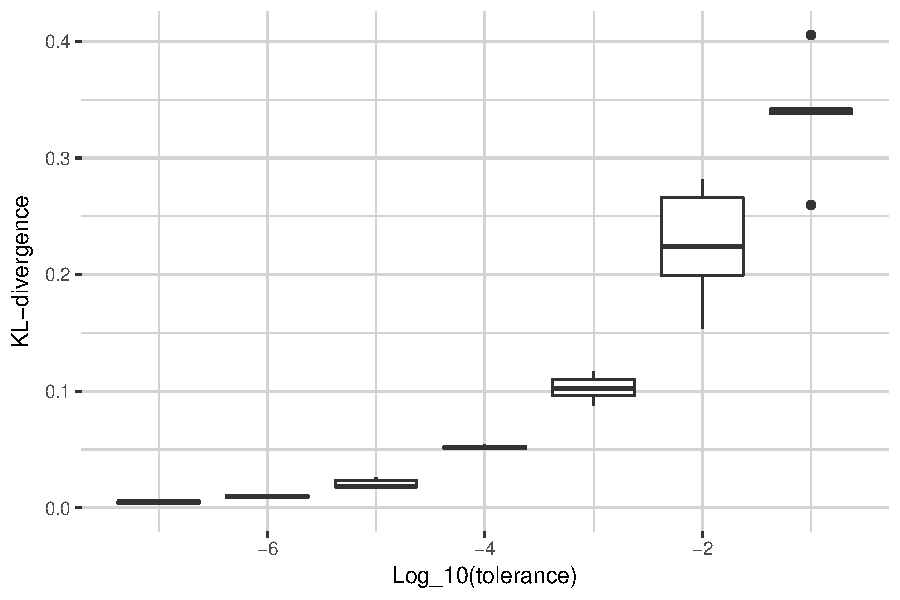
\includegraphics[width=\linewidth]{Figures/NearestNeighbor/Sequence/div_by_tol.pdf}
    	\caption{KL-divergence to true nearest neighbor distance distribution by tolerance, taken over 10 trials of the algorithm.}
    	\label{fig:NNDivergencesSequence}
	\end{subfigure}
    \begin{subfigure}{.49\textwidth}
    	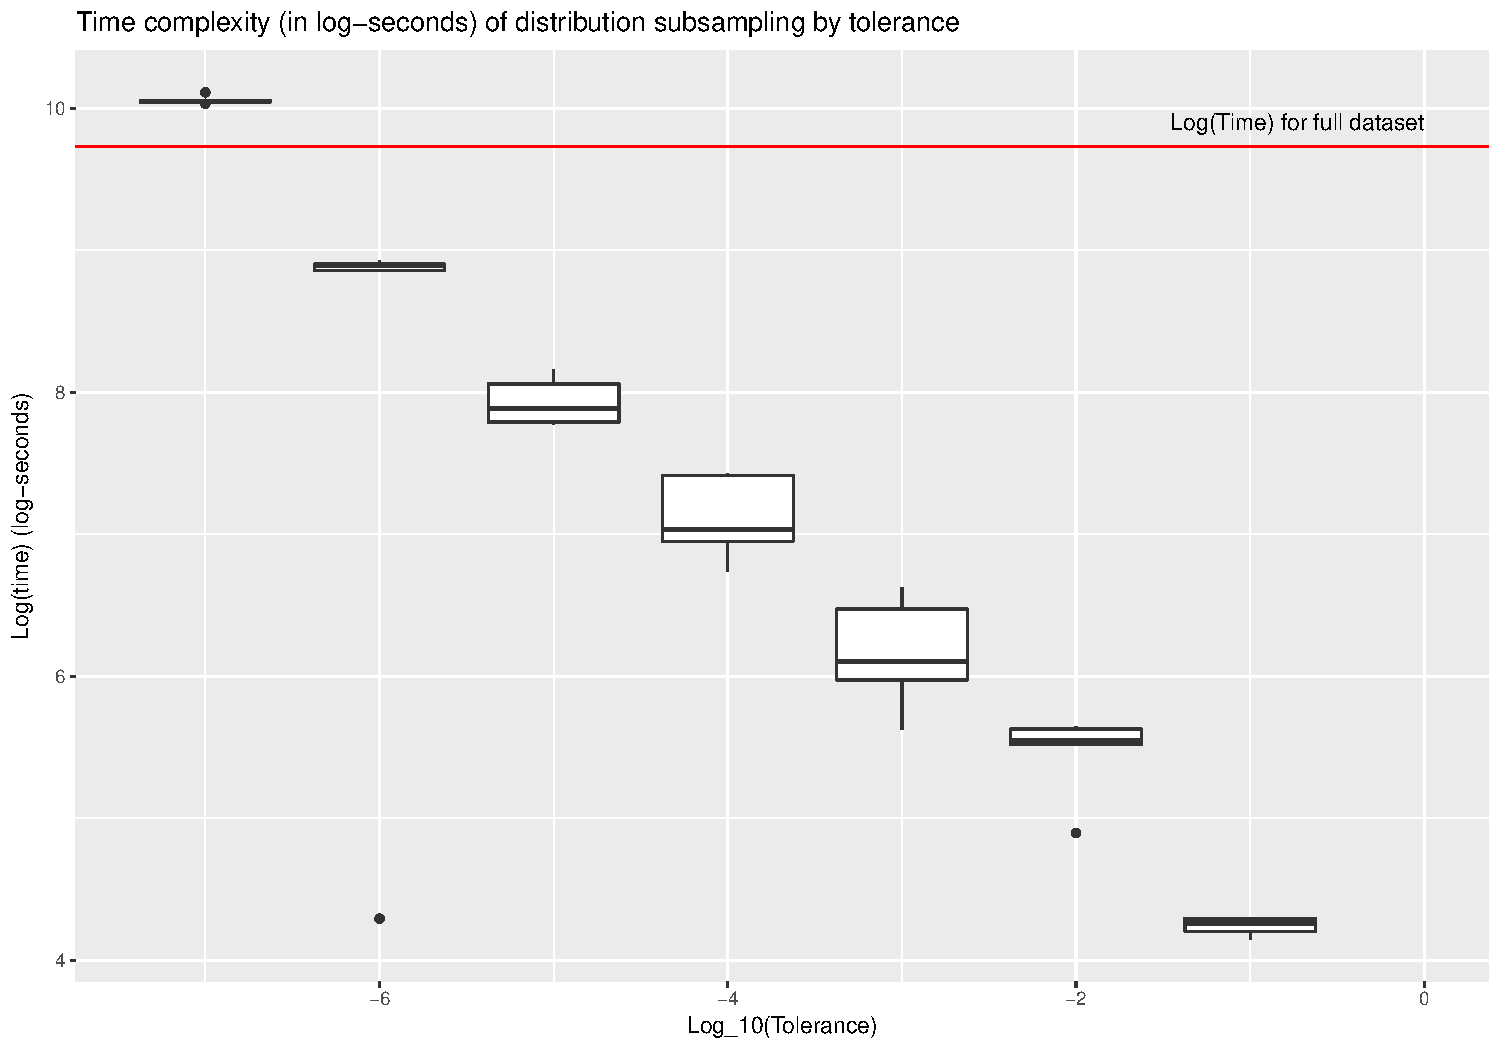
\includegraphics[width=0.9\linewidth]{Figures/NearestNeighbor/Sequence/log_time_by_tol.pdf}
    	\caption{Runtime (in seconds) and log-runtime (in log-seconds) for Algorithm~\ref{alg:DistributionAveraging} by tolerance, taken over 10 trials.}
    	\label{fig:NNTimesSequence}
    \end{subfigure}
    \caption{Performance of Algorithm~\ref{alg:NNDistributionAveraging} by tolerance applied to the nearest neighbor distribution of pairwise-aligned VDJ sequences.}
\end{figure}
It seems that the KL divergence to the truth may converge more slowly for \texttt{sequence\_alignment} sequences rather than CDR3s, although the approximate procedure seems to outperform the full distribution for a slightly larger range of $\varepsilon$ values (i.e. until $\varepsilon$ nears $10^{-6}$).


Next we investigate the effect of dataset size on the performance of Algorithm~\ref{alg:NNDistributionAveraging}.
For sample sizes $n \in \{\exp(6), \dots, \exp(10)\}$, we subsample \texttt{p\_f1} without replacement to $n$ sequences and compute the pairwise distance distribution of CDR3 sequences for the full subsampled dataset as well as those given by tolerances $\varepsilon \in \{0.1, ..., 10^{-5}\}$.
We perform this experiment 5 times for each $n$.

Figures~\ref{fig:NNDivBySizeCDR3}, \ref{fig:NNTimeBySizeCDR3}, and \ref{fig:NNEfficiencyBySizeCDR3} display boxplots of the KL-divergence to truth, runtime, and time efficiency, respectively.
\begin{figure}
	\begin{subfigure}{0.5\textwidth}
    	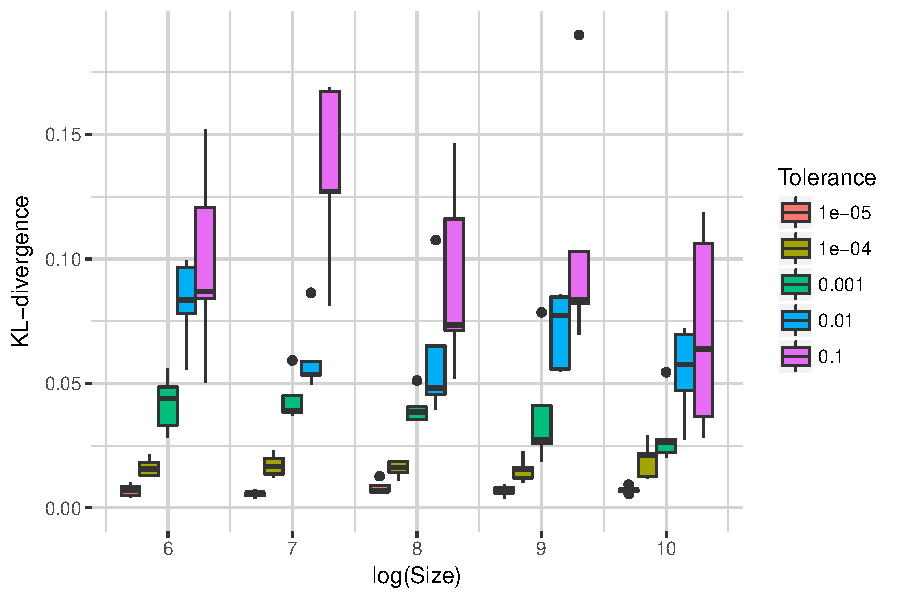
\includegraphics[width=\linewidth]{Figures/NearestNeighbor/CDR3/div_by_size_and_tol.pdf}
    	\caption{KL-divergence to true nearest neighbor distribution by tolerance and log(size) of dataset, taken over 10 trials of the algorithm.}
    	\label{fig:NNDivBySizeCDR3}
	\end{subfigure}
	\begin{subfigure}{0.5\textwidth}
    	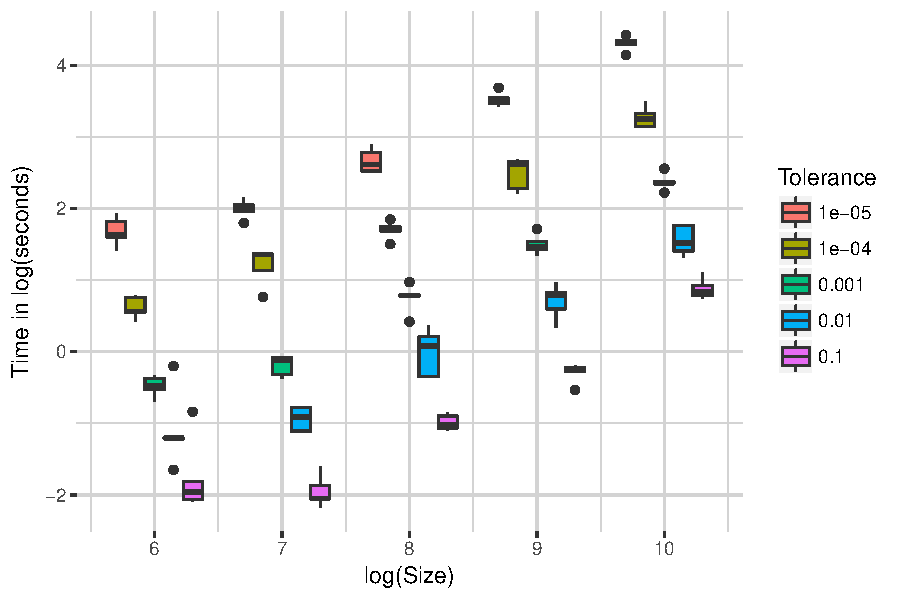
\includegraphics[width=\linewidth]{Figures/NearestNeighbor/CDR3/time_by_size_and_tol.pdf}
    	\caption{Time complexity of the approximate nearest neighbor distribution by tolerance and log(size) of dataset, taken over 10 trials of the algorithm.}
    	\label{fig:NNTimeBySizeCDR3}
    \end{subfigure}
    \begin{subfigure}{0.5\textwidth}
        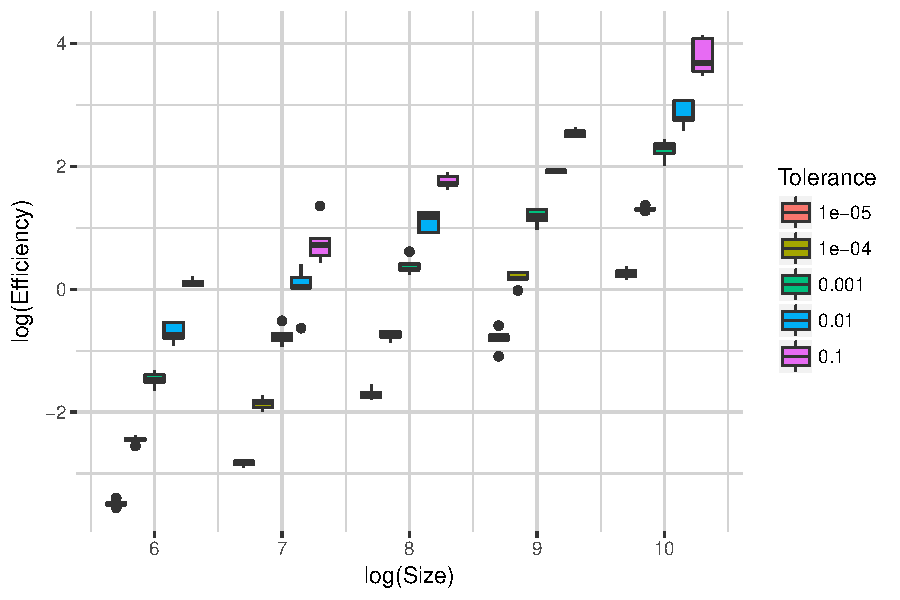
\includegraphics[width=\linewidth]{Figures/NearestNeighbor/CDR3/efficiency_by_size_and_tol.pdf}
    	\caption{KL-divergence to true nearest neighbor distribution by tolerance and log(size) of dataset, taken over 10 trials of the algorithm.}
    	\label{fig:NNEfficiencyBySizeCDR3}
    \end{subfigure}
    \caption{Performance of Algorithm~\ref{alg:NNDistributionAveraging} by sample size and tolerance applied to the nearest neighbor distribution of CDR3nt sequences.}
\end{figure}
There is not an obvious trend in KL divergence to truth for a given tolerance as sample size increases, although the variability is higher for high tolerances.
As expected, runtime increases as tolerance decreases, and also increases with the size of the dataset.
This is reasonable since each batch iteration of Algorithm~\ref{alg:NNDistributionAveraging} must compute the nearest neighbor distance from each sequence in batch $B$ to the full repertoire $R$, which certainly increases in time complexity as $R$ increases.

Next we look at the efficiency relative to computing the full distribution as defined in Equation~\ref{eq:Efficiency}.
Examining the boxplots near $y = 0$ by $\log(\text{size})$, we see that for a dataset of size $\exp(k)$, we would need a tolerance of at least $\frac{1}{10^{k - 4}}$.
For example, for $\log(\text{size}) = 6$, we see that tolerances higher than $0.01 = \frac{1}{100} = \frac{1}{10^{6 - 4}}$ would on average yield an efficiency greater than one.
This suggests that, for a dataset with $n$ CDR3 sequences, a sensible rule of thumb would be to choose $\varepsilon > \frac{1}{10^{k - 4}} = \frac{1}{10^{\log(n) - 4}}$.
This will of course be more or less appropriate for a given dataset depending on the nature of the repertoire from which it was sampled.

Finally, we perfrom the same experiment but using \texttt{sequence\_alignment} sequences for the nearest neighbor distance distribution.
Figures~\ref{fig:NNDivBySizeFull}, \ref{fig:NNTimeBySizeFull}, and \ref{fig:NNEfficiencyBySizeFull} display boxplots of the KL-divergence to truth, runtime, and time efficiency, respectively.
\begin{figure}
	\begin{subfigure}{0.5\textwidth}
    	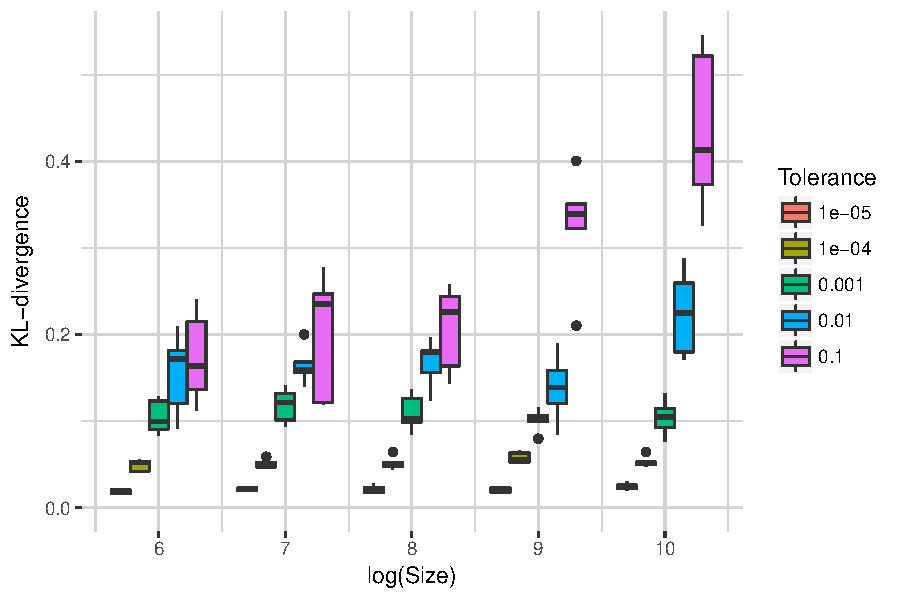
\includegraphics[width=\linewidth]{Figures/NearestNeighbor/Sequence/div_by_size_and_tol.pdf}
    	\caption{KL-divergence to true nearest neighbor distribution by tolerance and log(size) of dataset, taken over 10 trials of the algorithm.}
    	\label{fig:NNDivBySizeFull}
	\end{subfigure}
	\begin{subfigure}{0.5\textwidth}
    	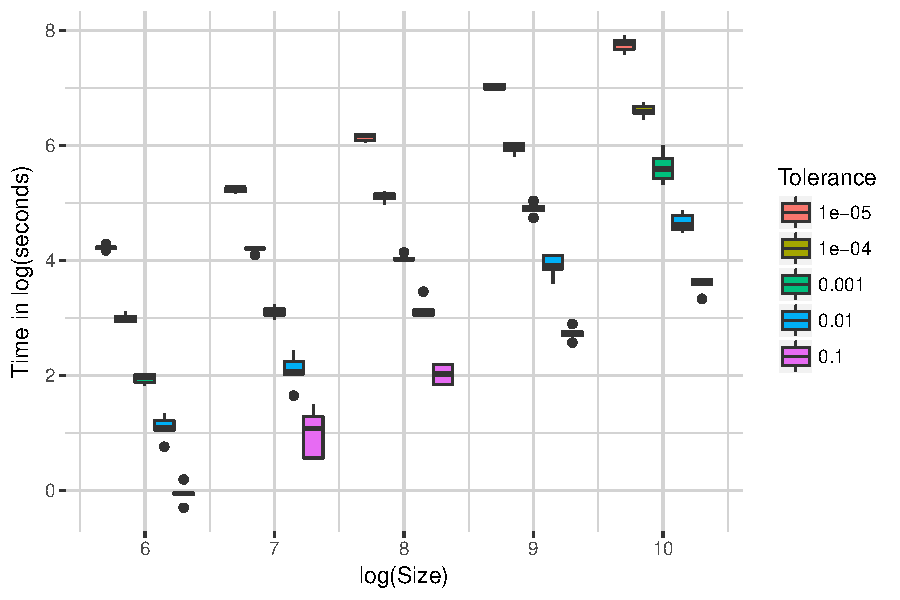
\includegraphics[width=\linewidth]{Figures/NearestNeighbor/Sequence/time_by_size_and_tol.pdf}
    	\caption{Time complexity of the approximate nearest neighbor distribution by tolerance and log(size) of dataset, taken over 10 trials of the algorithm.}
    	\label{fig:NNTimeBySizeFull}
    \end{subfigure}
    \begin{subfigure}{0.5\textwidth}
        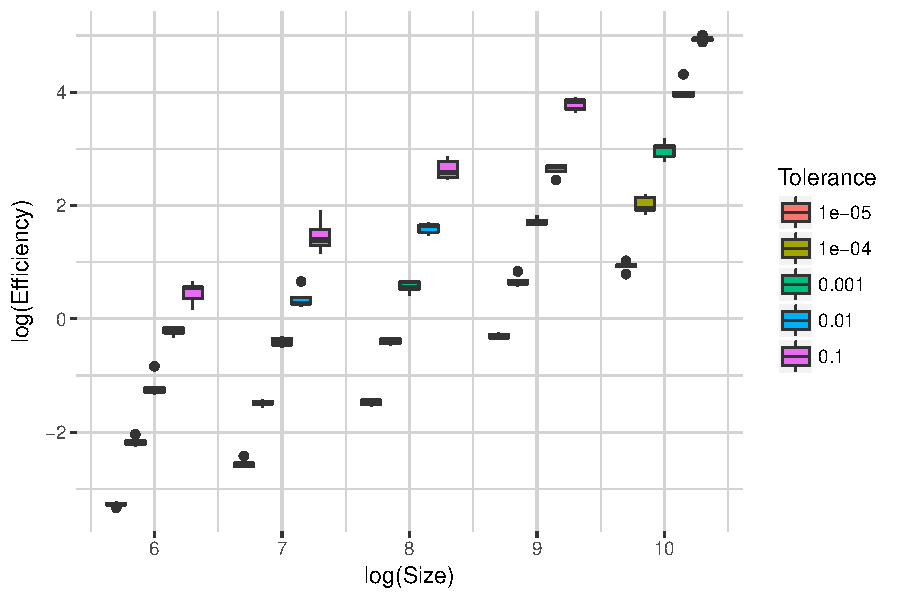
\includegraphics[width=\linewidth]{Figures/NearestNeighbor/Sequence/efficiency_by_size_and_tol.pdf}
    	\caption{KL-divergence to true nearest neighbor distribution by tolerance and log(size) of dataset, taken over 10 trials of the algorithm.}
    	\label{fig:NNEfficiencyBySizeFull}
    \end{subfigure}
     \caption{Performance of Algorithm~\ref{alg:NNDistributionAveraging} by sample size and tolerance applied to the nearest neighbor distribution of pairwise-aligned VDJ sequences.}
\end{figure}
There is evidence of a positive trend of the KL-divergence as sample size increases for $\varepsilon = 0.1$, although this trend seems to diminish for each other tolerance.
Runtimes increase with given sample size and tolerance, and are generally higher than they are for \texttt{junction} sequences as expected.
It turns out that the efficiencies follow the same rule of thumb we derived for the \texttt{junction} sequence situation.
In particular, choosing $\varepsilon > \frac{1}{10^{k - 4}} = \frac{1}{10^{\log(n) - 4}}$ will on average lead to an increase in efficiency with respect to the full distribution for \texttt{sequence\_alignment} sequences as well as \texttt{junction} sequences.
While this may depend on the dataset in question, we recommend this as a good point of reference for general use.

The user should use these results as well as problem-specific considerations when deciding whether or not to use Algorithm~\ref{alg:NNDistributionAveraging} instead of computing the full distribution, and if so, which tolerance to use.

\subsection*{Appendix C: Model validation analysis workflows}
Figure~\ref{fig:IgorWorkflow} illustrates the \texttt{igor} model validation workflow.
We employ IgBlast to obtain CDR3 sequences for the observed sequences, which \igor\ only outputs for generated sequences.
Moreover, because we fit \igor\ models on predominantly functional TRB sequences, we consider only \igor\-generated sequences whose V and J segments are in-frame.  

%EM Hm, isn't CDR3 pretty obvious? (I'm not sure but that was my impression)
%BJO - That was my thought too, but I'm not 100% sure these two tools would always infer the same CDR3.
% Hence, the resultant analysis can be thought to validate a joint modeling effort between \texttt{igor} and IgBlast to whatever extent IgBlast introduces bias in CDR3 inferences.
\begin{figure}
	\begin{subfigure}{0.5\textwidth}
        \begin{adjustbox}{max totalsize={\textwidth}{.5\textheight},center}
            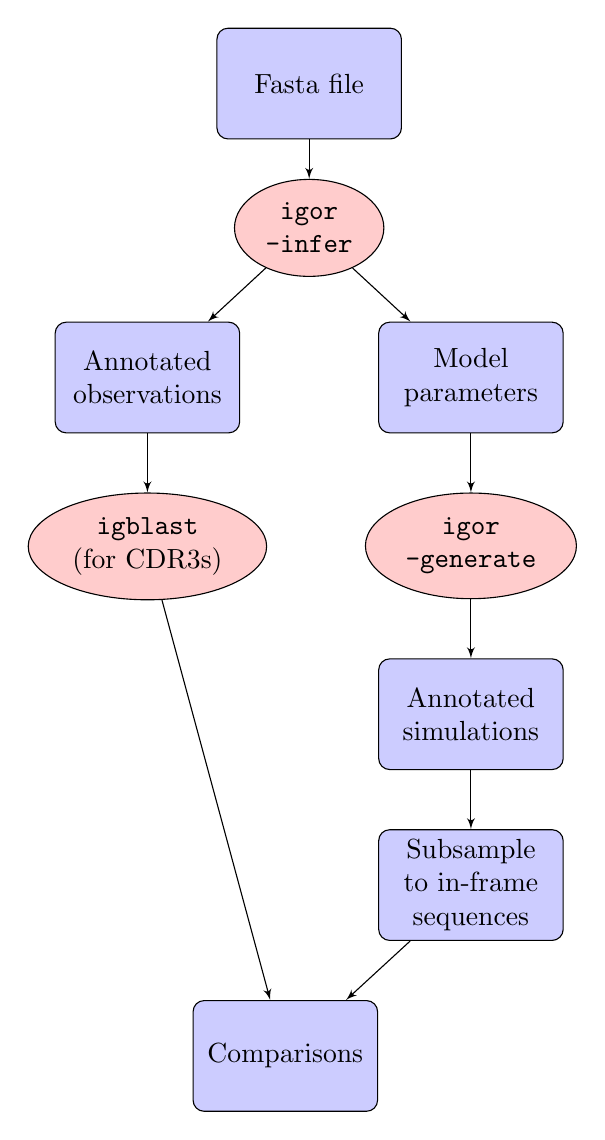
\begin{tikzpicture}
                \node[block](fasta){Fasta file};
                \node[cloud, below =0.5 cm of fasta, align=center](igor){\texttt{igor}\\ \texttt{-infer}};
                \node[block, below left=0.75 cm and 0.2 cm of igor](igordata){Annotated observations};
                \node[cloud, below=0.75cm of igordata, align=center](igblast){\texttt{igblast}\\ (for CDR3s)} ;
                \node[block, below right=0.75 cm and 0.2 cm of igor](params){Model parameters};
                \node[cloud, below=0.75cm of params, align=center](simulate){\texttt{igor} \\ \texttt{-generate}};
                \node[block, below = 0.75cm of simulate](sim){Annotated simulations};
                \node[block, below = 0.75cm of sim](subsample){Subsample to in-frame sequences};
                \node[block, below left=0.75 cm  and 0 cm of subsample](c1){Comparisons};
                \path[line](fasta) -- (igor);
                \path[line] (igor) -- (igordata);
                \path[line] (igor) -- (params);
                \path[line] (params) -- (simulate);
                \path[line] (simulate) -- (sim);
                \path[line] (igordata) -- (igblast);
                \path[line] (igblast) -- (c1);
                \path[line] (sim) -- (subsample);
                \path[line] (subsample) -- (c1);
            \end{tikzpicture}
        \end{adjustbox}
        \caption{Workflow for comparing a given observed repertoire dataset to an example simulated dataset via \igor.}
        \label{fig:IgorWorkflow}
    \end{subfigure}
    \begin{subfigure}{0.5\textwidth}
    \begin{adjustbox}{max totalsize={\textwidth}{.5\textheight},center}
        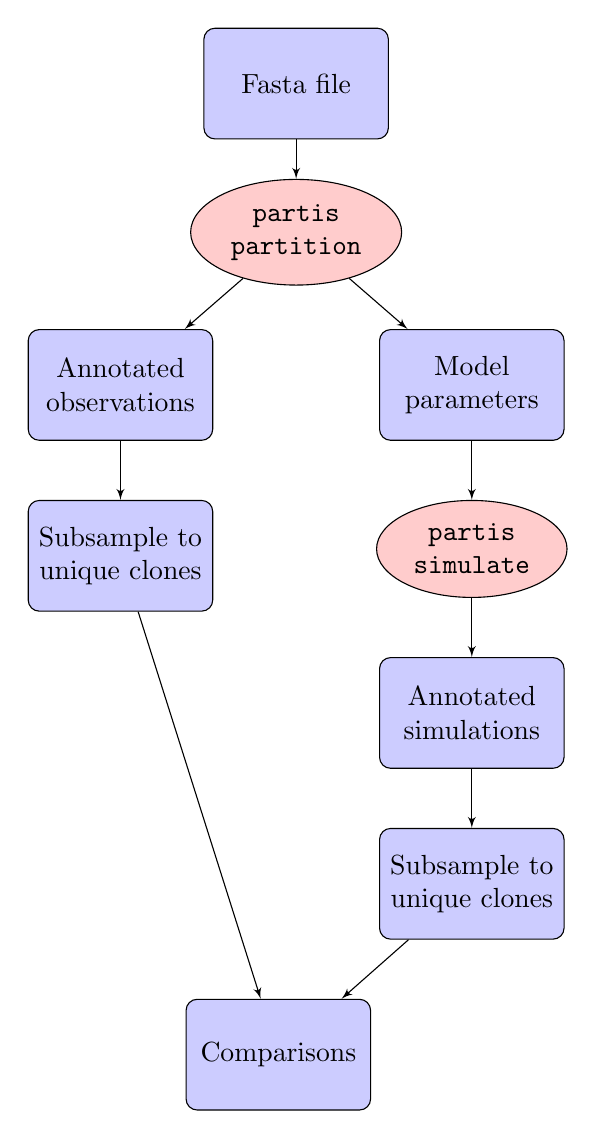
\begin{tikzpicture}
            \node[block](fasta){Fasta file};
            \node[cloud, below =0.5 cm of fasta, align=center](partis){\texttt{partis}\\ \texttt{partition}};
            \node[block, below left=0.75 cm and 0.1 cm of partis](partisdata){Annotated observations};
            \node[block, below = 0.75 cm of partisdata](clones){Subsample to unique clones};
            \node[block, below right=0.75 cm and 0.1 cm of partis](params){Model parameters};
            \node[cloud, below=0.75cm of params, align=center](simulate){\texttt{partis} \\ \texttt{simulate}};
            \node[block, below = 0.75cm of simulate](sim){Annotated simulations};
            \node[block, below = 0.75cm of sim](simclones){Subsample to unique clones};
            \node[block, below left=0.75 and 0.1cm of simclones](c1){Comparisons};
            \path[line](fasta) -- (partis);
            \path[line] (partis) -- (partisdata);
            \path[line] (partis) -- (params);
            \path[line] (params) -- (simulate);
            \path[line] (simulate) -- (sim);
            \path[line] (partisdata) -- (clones);
            \path[line] (clones) -- (c1);
            \path[line] (sim) -- (simclones);
            \path[line] (simclones) -- (c1);
        \end{tikzpicture}
    \end{adjustbox}
    \caption{Workflow for comparing a given observed repertoire dataset to an example simulated dataset via \texttt{partis}.}
    \label{fig:PartisWorkflow}
    \end{subfigure}
    \caption{Workflow diagrams for the \igor\ and \partis\ model validation analyses.}
\end{figure}
Figure~\ref{fig:PartisWorkflow} illustrates the \texttt{partis} model validation workflow as described in the Methods section.
We first run \texttt{partis partition} on each fasta file of IgH sequence reads to obtain annotations for each sequence, as well as a directory containing model parameters for inference and simulation.
We can then run \texttt{partis simulate} with these model parameters as input to generate a synthetic datset of IgH annotations.
We subsample both the experimental and simulated annotation datasets to unique clones.
Then, we compare each IgH-relevant summary for the two resultant annotations datasets, yielding a divergence value for each summary.


\subsection*{Appendix D: Comparison of summary scores using IgBlast annotations}
Recall that for the standard \texttt{partis} model validation procedure, \texttt{partis} is used for both inference as well as simulation.
Here we examine the influence of using the same tool for inference and simulation by using IgBlast for inference, and comparing the annotations dataset output from IgBlast to the corresponding simulations from \texttt{partis}.
The workflow for this procedure is displayed in Figure~\ref{IgblastWorkflow}, which is essentially the diagram in Figure~\ref{fig:PartisWorkflow} with an additional path describing the IgBlast/Change-O pipeline.
%BJO - It might be worth also including a box called "IMGT database" as another input (along with "Fasta file")
\begin{figure}
    \begin{adjustbox}{max totalsize={\textwidth}{.8\textheight},center}
        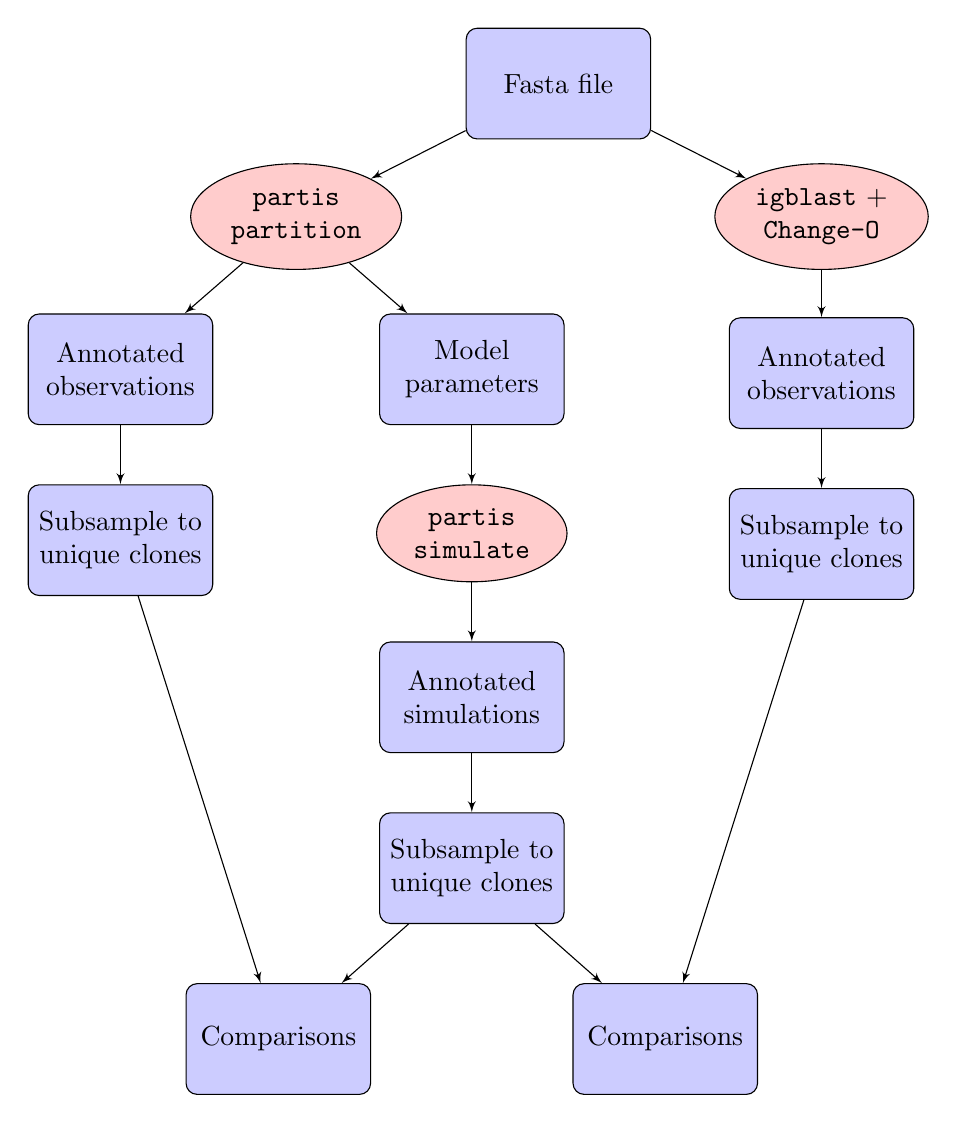
\begin{tikzpicture}
        \node[block](fasta){Fasta file};
        \node[cloud, below left=0.5 cm and 1.2 cm of fasta, align=center](partis){\texttt{partis}\\ \texttt{partition}};
        \node[block, below left=0.75 cm and 0.1 cm of partis](partisdata){Annotated observations};
        \node[block, below = 0.75 cm of partisdata](clones){Subsample to unique clones};
        \node[block, below right=0.75 cm and 0.1 cm of partis](params){Model parameters};
        \node[cloud, below=0.75cm of params, align=center](simulate){\texttt{partis} \\ \texttt{simulate}};
        \node[block, below = 0.75cm of simulate](sim){Annotated simulations};
        \node[block, below = 0.75cm of sim](simclones){Subsample to unique clones};
        \node[block, below left=0.75 and 0.1cm of simclones](c1){Comparisons};
        \path[line](fasta) -- (partis);
        \path[line] (partis) -- (partisdata);
        \path[line] (partis) -- (params);
        \path[line] (params) -- (simulate);
        \path[line] (simulate) -- (sim);
        \path[line] (partisdata) -- (clones);
        \path[line] (clones) -- (c1);
        \path[line] (sim) -- (simclones);
        \path[line] (simclones) -- (c1);
            \node[cloud, below right=0.5 cm and 1.2 cm of fasta, align=center](igblast){\texttt{igblast} + \\ \texttt{Change-O}};
            \node[block, below=0.6 cm of igblast](igblastdata){Annotated observations};
            \node[block, below = 0.75 cm of igblastdata](igblastclones){Subsample to unique clones};
            \node[block, below right=0.75 and 0.1cm of simclones](c2){Comparisons};
            \path[line](fasta) -- (igblast);
            \path[line] (igblast) -- (igblastdata);
            \path[line] (igblastdata) -- (igblastclones);
            \path[line] (igblastclones) -- (c2);
            \path[line] (simclones) -- (c2);
        \end{tikzpicture}
    \end{adjustbox}
    \caption{Workflow diagram for \partis\ model validation when comparing \texttt{partis} and \texttt{igblast} annotations to partis simulations}
    \label{IgblastWorkflow}
\end{figure}
Change-O was used to parse the \texttt{igblast} output, as well as partition the sequences into inferred clonal families \cite{Gupta2015-iu}.

Figure~\ref{fig:IgBlastScores} shows the results of score$_\text{obs}$ by summary when using IgBlast for annotation and \texttt{partis} for simulation.
Figure~\ref{fig:ScoreDiffs} shows the difference of each score in Figure~\ref{fig:ObsScoresBCR} and each score in Figure~\ref{fig:IgBlastScores}.
\begin{figure}
	\begin{subfigure}{\textwidth}
   		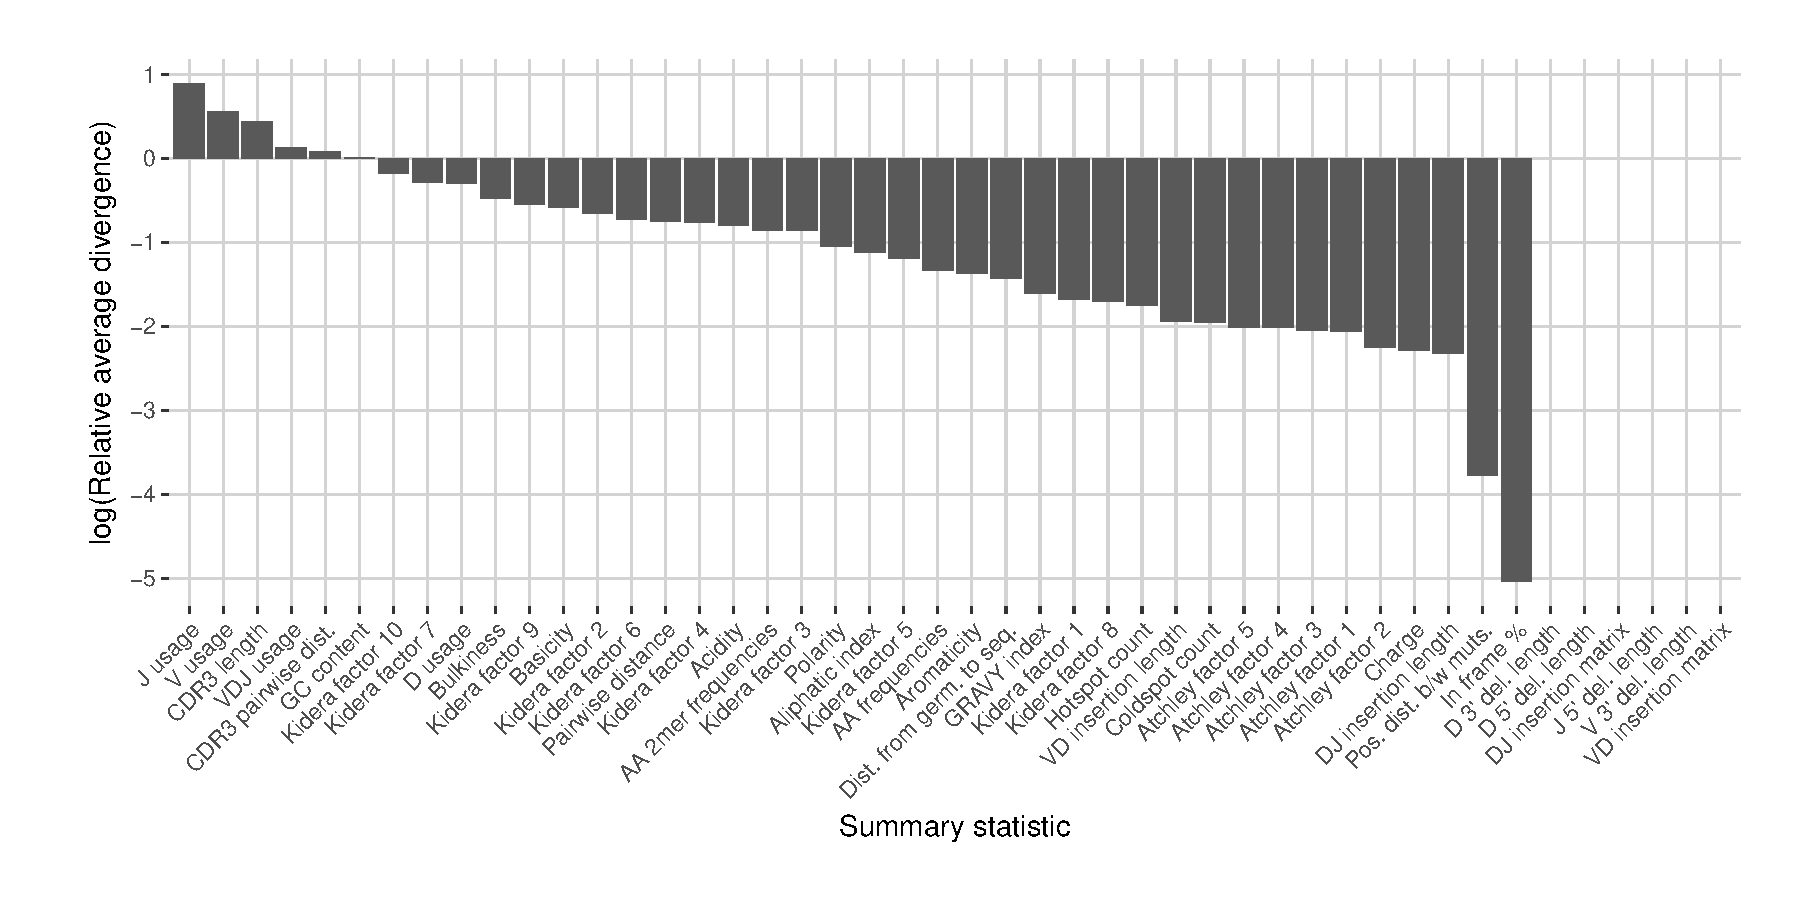
\includegraphics[width=\linewidth]{Figures/PartisScores/obs_score_plot_igb.pdf}
    	\caption{Comparing divergences for \texttt{igblast} annotations and \texttt{partis} simulations based on the same individual observed repertoires.
    	    We use the default germline databases in \texttt{igblast} for consistency.
    	}
    	\label{fig:IgBlastScores}
	\end{subfigure}
	\begin{subfigure}{\textwidth}
   		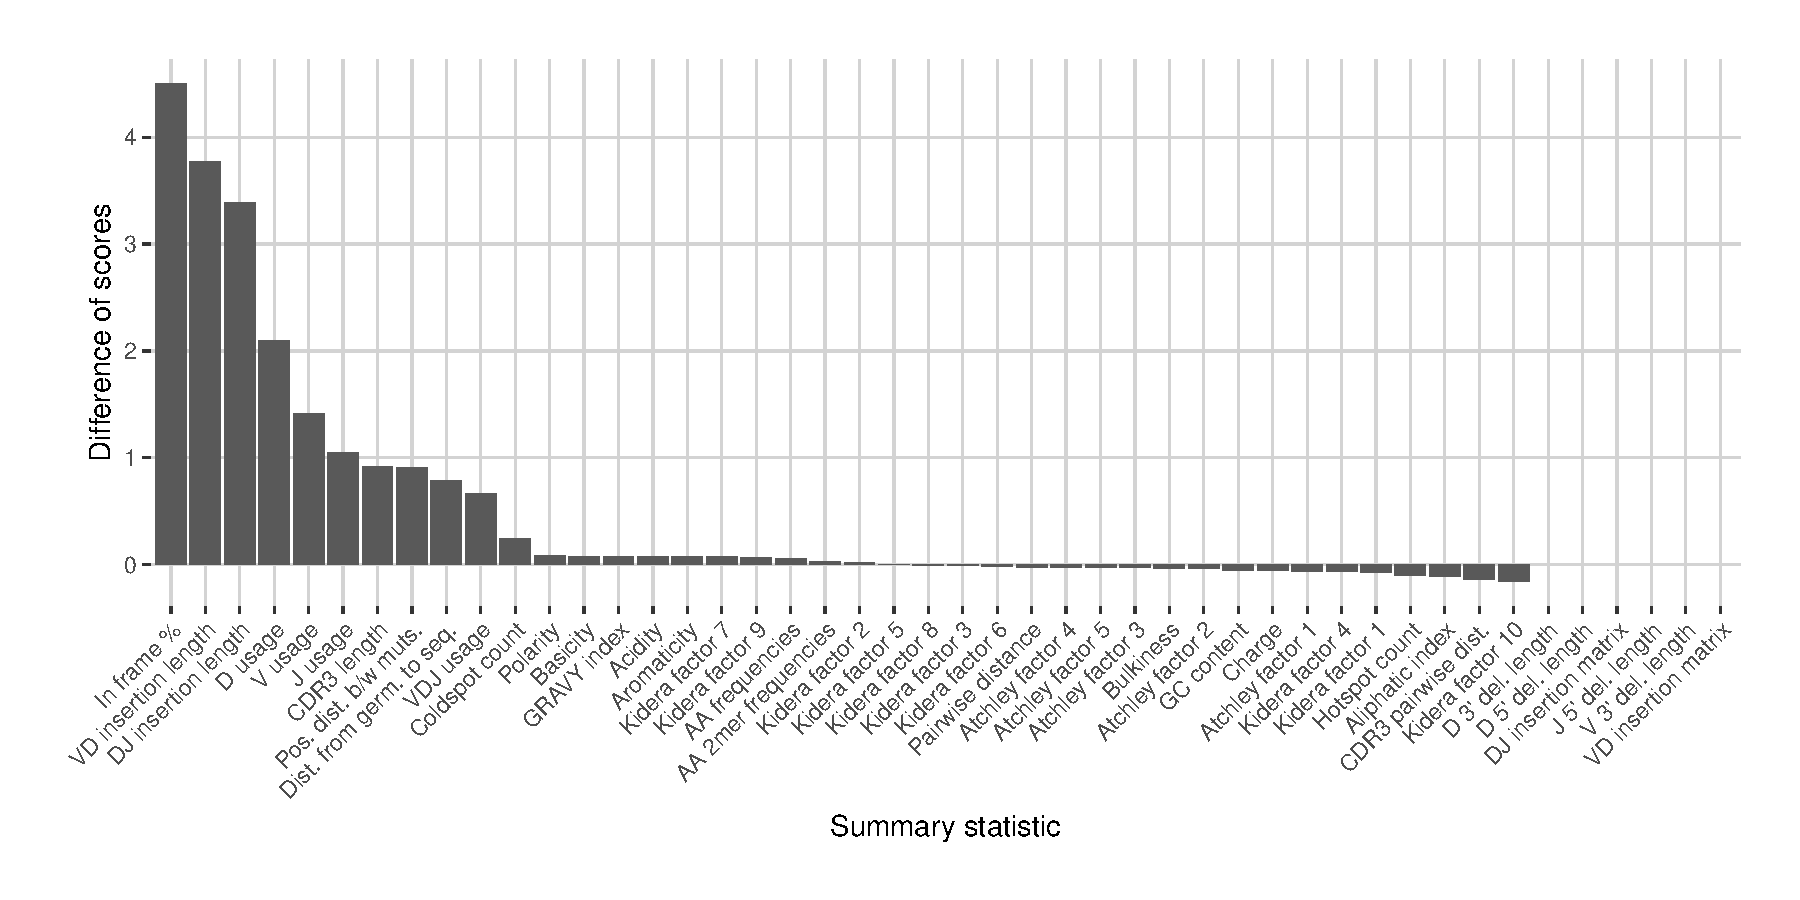
\includegraphics[width=\linewidth]{Figures/PartisScores/score_diff.pdf}
    	\caption{Difference in score$_\text{obs}$ values when using \texttt{igblast} versus \texttt{partis} for annotations.
    	}
    	\label{fig:ScoreDiffs}
	\end{subfigure}
	\caption{Summary scores for each statistic in the \partis\ model validation experiment when comparing \partis\ simulations to \igblast\ annotations.
	IMGT IgH germline databases were used during inference for both tools.
	In both plots, a high score indicates a well-replicated statistic by the simulations with respect to their corresponding experimental repertoires of functional IgH sequences.
	Summaries without a score are not readily available from AIRR-formatted \igblast\ output.
	}
\end{figure}
Frequency polygons of three pairs of \igblast-annotated and \partis-simulated datasets are shown in Figure~\ref{fig:PartisIgBlastFreqpolys}, and ecdfs of the same datasets are shown in Figure~\ref{fig:PartisIgBlastECDFs}
The plots show a high level of agreement for most summaries, with all but six of them differing by less than one units, and a strong majority of them close to zero.
Where differences arise, this is likely the result of differences in how partis and IgBlast perform annotations.
For example, we see that the insertion length distributions highly disagree in scores.
This is at least partially attributable to the star-tree assumption on which \texttt{partis} operates, which is prone to overestimate insertion lengths in an effort to better estimate the ultimate naive sequence.
Indeed, examining the VD insertion length distribution shows that IgBlast tends to assign a similar distribution to each dataset, whereas partis leads to more variable distributions with right skew due to the star-tree assumption.
Moreover, if IgBlast tends to assign a similar insertion length distribution to every dataset, then this will make it difficult for a simulator designed to match particular insertion lengths distributions to behave more like the IgBlast distributions.
Thus, inherent differences in annotation tools will certainly lead to differences in summary scores, regardless of how accurate either tool is.
Hence, it is important to understand that a given annotations-based summary should be considered in the context of the tool which provided annotations, and not as a ground-truth summary of the actual gene usage/indel statistics.

\begin{figure}
    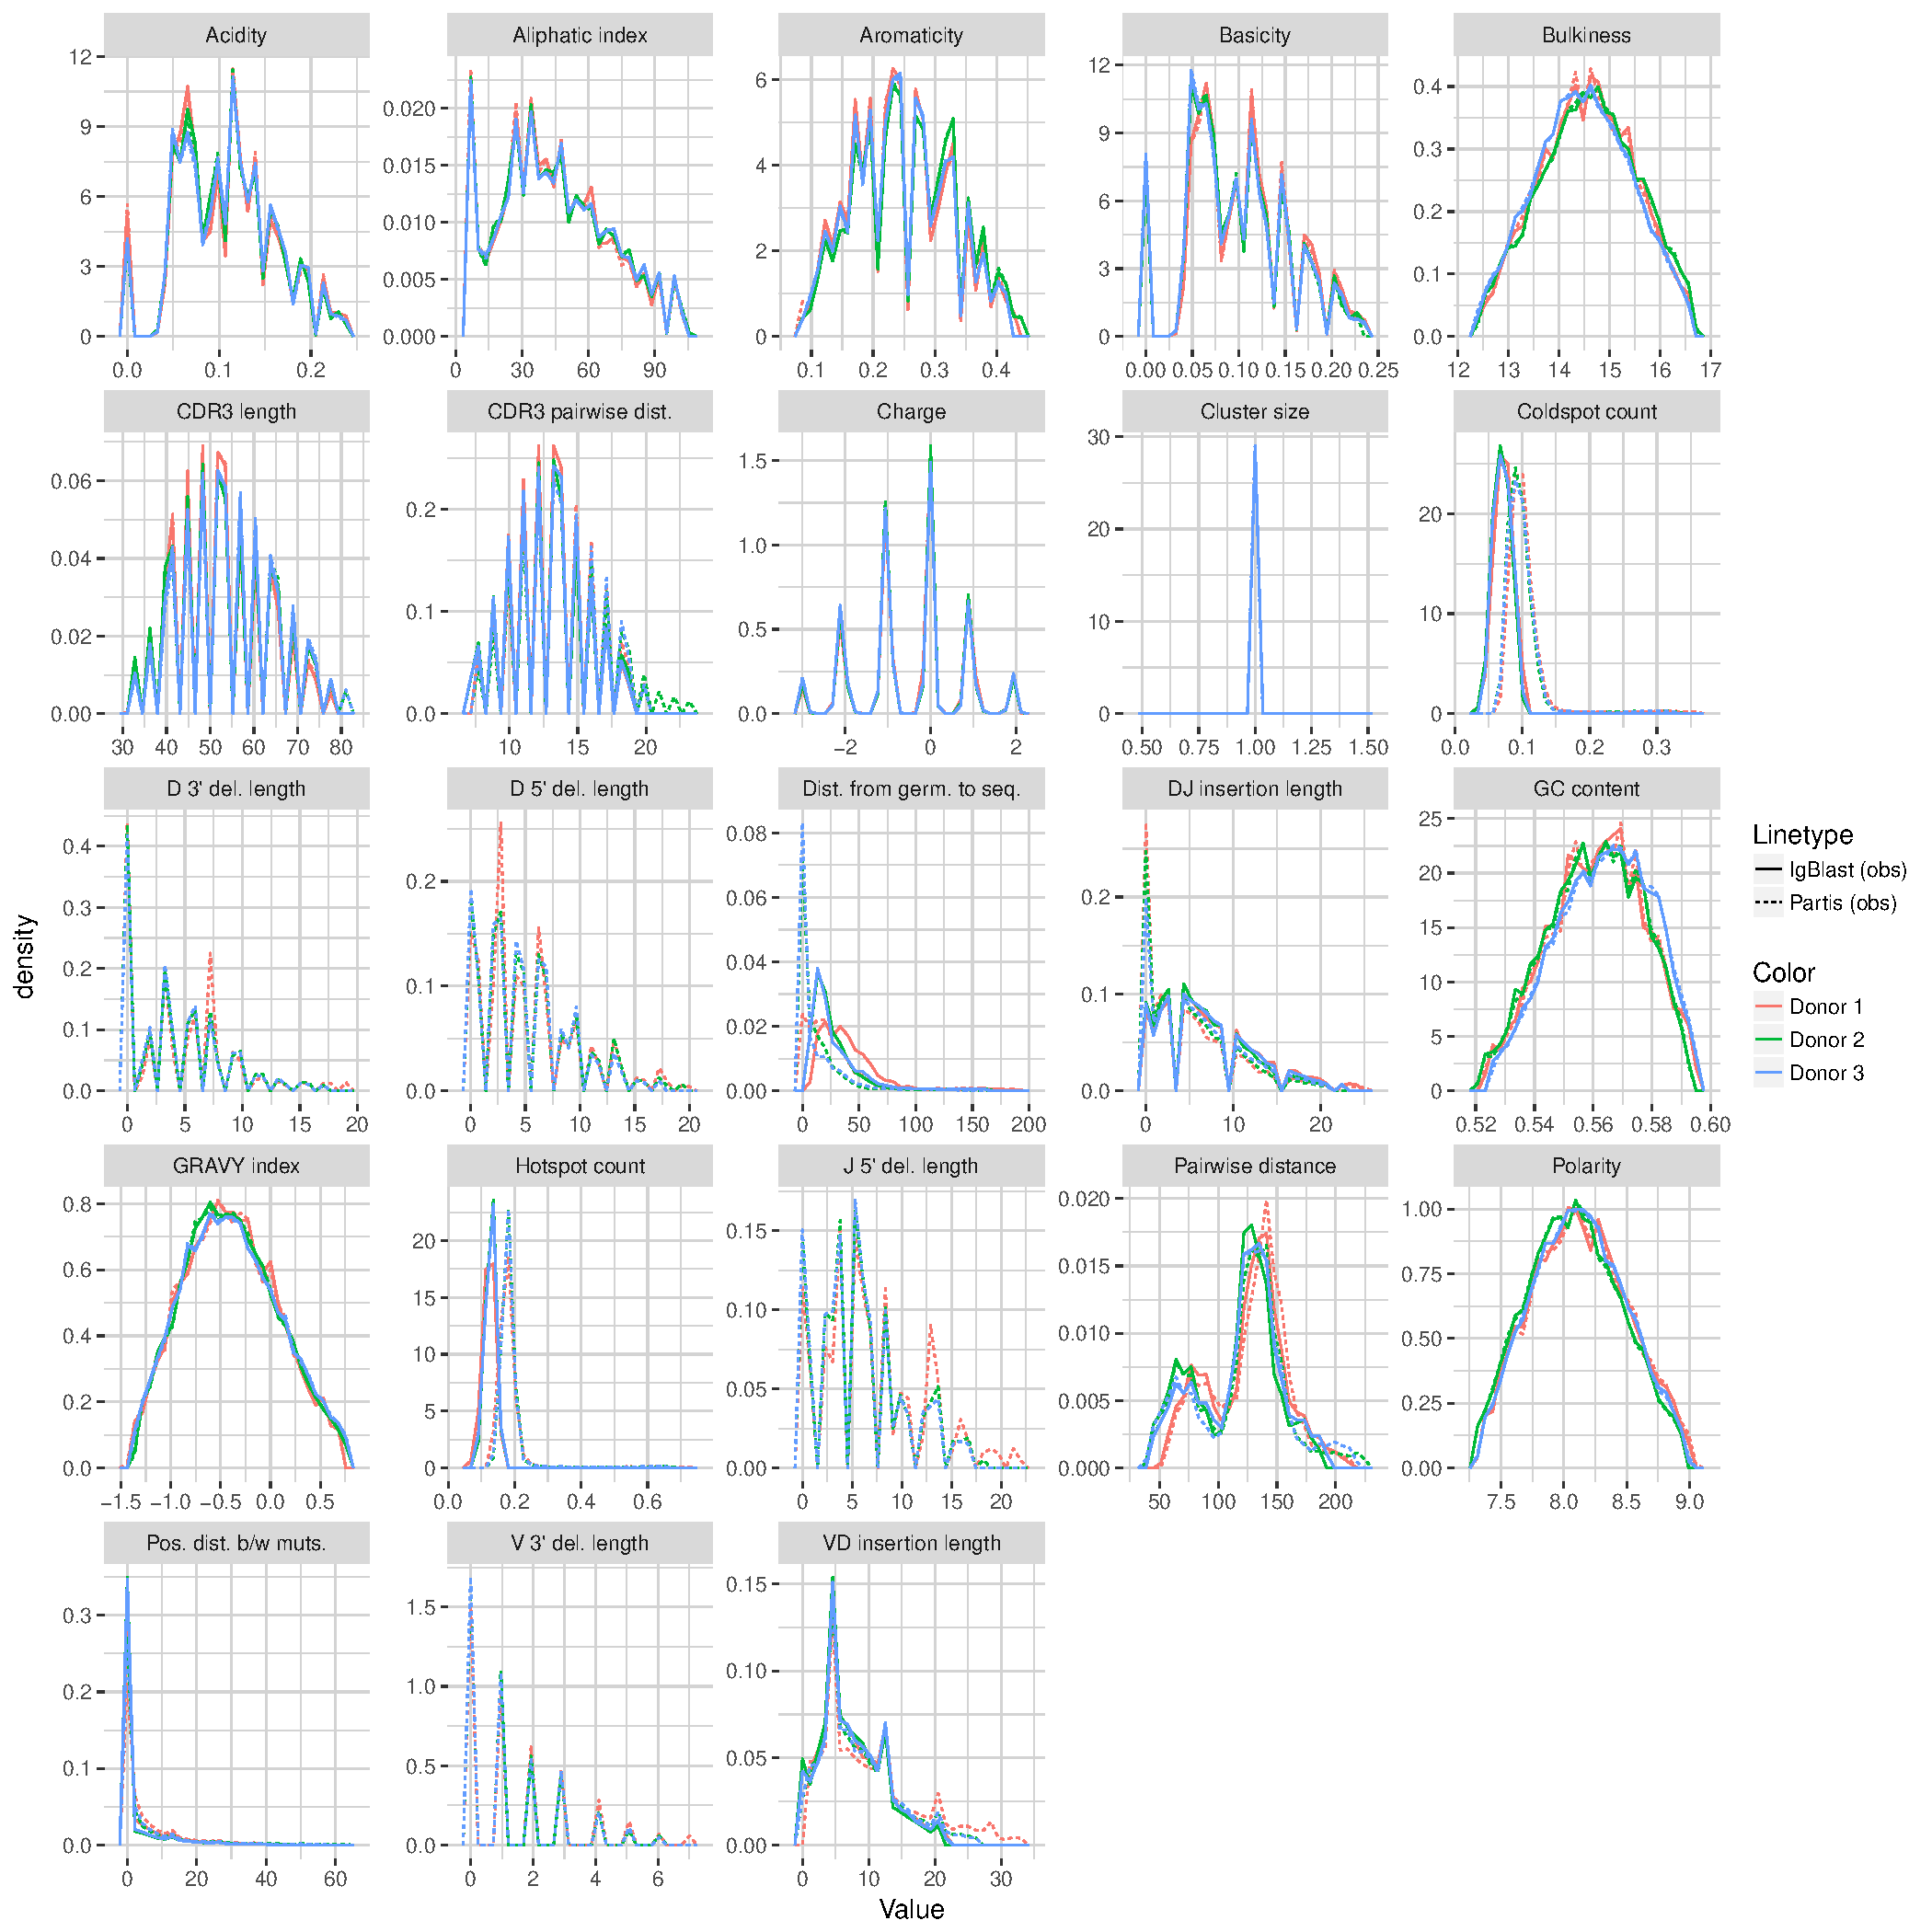
\includegraphics[width=\linewidth]{Figures/PartisScores/pi_freqpoly.pdf}
    \caption{Summary distribution frequency polygons of three datasets based on \texttt{partis} versus \texttt{igblast} annotations.}
    \label{fig:PartisIgBlastFreqpolys}
\end{figure}

\begin{figure}
    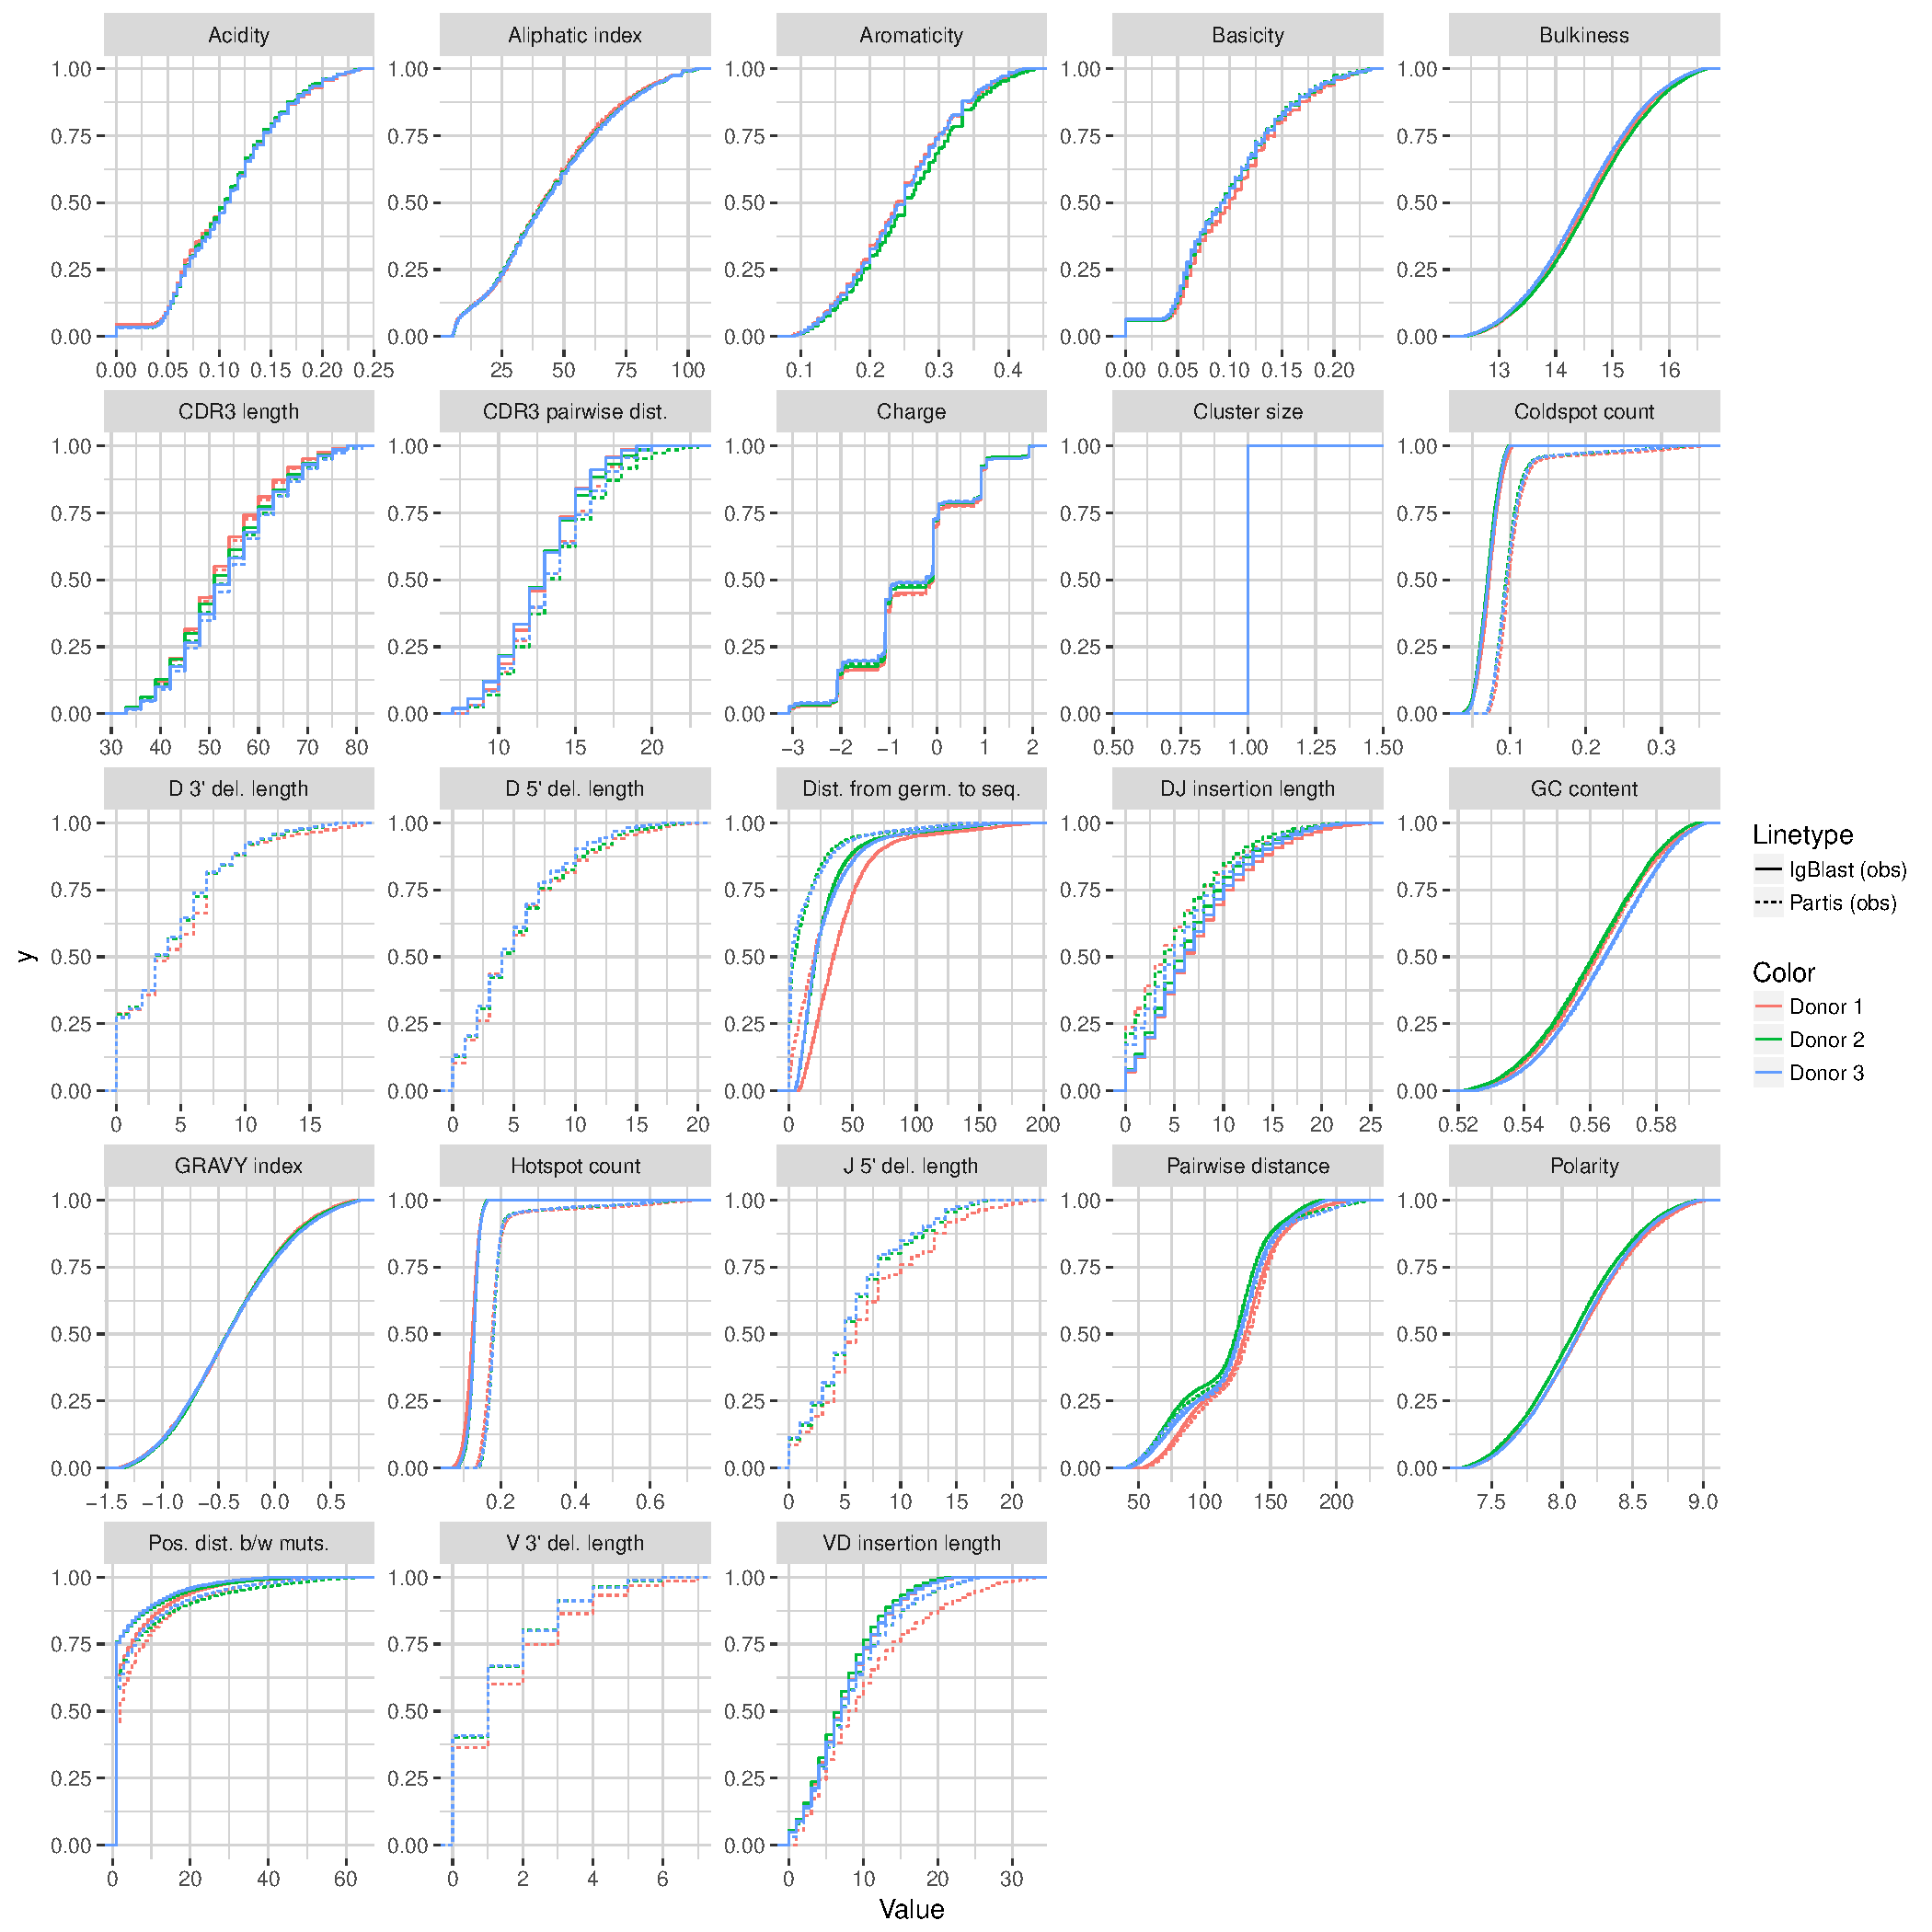
\includegraphics[width=\linewidth]{Figures/PartisScores/pi_ecdf.pdf}
    \caption{Summary distribution empirical cdfs of three datasets based on \texttt{partis} versus \texttt{igblast} annotations.}
     \label{fig:PartisIgBlastECDFs}
\end{figure}

%BJO - I'm not actually sure how necessary this table is anymore, since I removed the divergence plot which used these abbreviations as axis labels. Everything just gets rolled up into the score plots and freqpolys/ecdfs now.
%BJO - p_f1 does show up in the subsampling performance analyses in Appendices A and B.
\section*{Appendix E: Metadata for partis analysis}

Table~\ref{tab:Datasets} gives metadata for each dataset used in the following analyses.
In short, the notation is as follows.
A prefix of \texttt{p} corresponds to \texttt{partis} annotations, a prefix of \texttt{i} corresponds to \texttt{igblast} annotations, and a prefix of \texttt{pi} corresponds to \texttt{partis} annotations using the default IMGT germline databases for IgBlast;
this is followed by a letter representing the individual succeeded by a number corresponding to the time point;
finally, we append the \texttt{sim} suffix if the dataset was simulated from an individual's inferred model parameters.
\begin{table}
\makebox[\textwidth][c]{
\begin{tabular}{c|c|c|c|c|c}
	Dataset label & Dataset type & Annotation tool & Germline set & Individual & Time point \\
	\hline
    \texttt{p\_f1} & Observation &     \texttt{partis} & \texttt{partis} & F & 1 hour \\
    \texttt{p\_f2} & Observation &     \texttt{partis} & \texttt{partis} & F & 8 days \\
    \texttt{p\_g1} & Observation &     \texttt{partis} & \texttt{partis} & G & 1 hour \\
    \texttt{p\_g2} & Observation &     \texttt{partis} & \texttt{partis} & G & 8 days \\
    \texttt{p\_i1} & Observation &     \texttt{partis} & \texttt{partis} & I & 1 hour \\
    \texttt{p\_i2} & Observation &     \texttt{partis} & \texttt{partis} & I & 8 days \\
    \texttt{i\_f1} & Observation &     \texttt{igblast} & IMGT & F & 1 hour \\
    \texttt{i\_f2} & Observation &     \texttt{igblast} & IMGT & F & 8 days \\
    \texttt{i\_g1} & Observation &     \texttt{igblast} & IMGT & G & 1 hour\\
    \texttt{i\_g2} & Observation &     \texttt{igblast} & IMGT & G & 8 days\\
    \texttt{i\_i1} & Observation &     \texttt{igblast} & IMGT & I & 1 hour\\
    \texttt{i\_i2} & Observation &     \texttt{igblast} & IMGT & I & 8 days\\
    \texttt{pi\_f1} & Observation &    \texttt{partis} & IMGT & F & 1 hour\\
    \texttt{pi\_f2} & Observation &    \texttt{partis} & IMGT & F & 8 days\\
    \texttt{pi\_g1} & Observation &    \texttt{partis} & IMGT & G & 1 hour\\
    \texttt{pi\_g2} & Observation &    \texttt{partis} & IMGT & G & 8 days\\
    \texttt{pi\_i1} & Observation &    \texttt{partis} & IMGT & I & 1 hour\\
    \texttt{pi\_i2} & Observation &    \texttt{partis} & IMGT & I & 8 days\\
    \texttt{p\_f1\_sim} & Simulation & \texttt{partis} & \texttt{partis} & F & 1 hour\\
    \texttt{p\_f2\_sim} & Simulation & \texttt{partis} & \texttt{partis} & F & 8 days\\
    \texttt{p\_g1\_sim} & Simulation & \texttt{partis} & \texttt{partis} & G & 1 hour\\
    \texttt{p\_g2\_sim} & Simulation & \texttt{partis} & \texttt{partis} & G & 8 days\\
    \texttt{p\_i1\_sim} & Simulation & \texttt{partis} & \texttt{partis} & I & 1 hour\\
    \texttt{p\_i2\_sim} & Simulation & \texttt{partis} & \texttt{partis} & I & 8 days\\
    \texttt{pi\_f1\_sim} & Simulation& \texttt{partis} & IMGT & F & 1 hour\\
    \texttt{pi\_f2\_sim} & Simulation& \texttt{partis} & IMGT & F & 8 days\\
    \texttt{pi\_g1\_sim} & Simulation& \texttt{partis} & IMGT & G & 1 hour\\
    \texttt{pi\_g2\_sim} & Simulation& \texttt{partis} & IMGT & G & 8 days\\
    \texttt{pi\_i1\_sim} & Simulation& \texttt{partis} & IMGT & I & 1 hour\\
    \texttt{pi\_i2\_sim} & Simulation& \texttt{partis} & IMGT & I & 8 days\\
\end{tabular}
}
\caption{Metadata for each dataset used in the BCR analyses}
\label{tab:Datasets}
\end{table}


\end{document}
